\documentclass[11pt,openright,twoside,a4paper]{report}

% These are the includes required for the doc 
%% Package to includes to provide additional functionality to the dissertation document
\usepackage{harvard}    	% Uses harvard style referencing
\usepackage{graphicx}   	% Permits import of various graphics formats
\usepackage{multicol}   	% Provides ability to split output into columns
\usepackage{listings}   	% Provides styled code listings
\usepackage{minted}         % Minted theme for code listings
\usepackage{xcolor}         % Set background colours for code listings
\usepackage{float}      	% Suppresses floating for tables and figures when using "H"
\usepackage{etoolbox}   	% enable bibliography to be added to the table of contents
\usepackage{comment}    	% enable block of comments
\usepackage{enumitem}       % resume enumerations
\usepackage{breakurl}       % used to break long url links
\usepackage{longtable}      % span tables through multiple pages. Note: It may be necessary to compile the document several times to get a multi-page table to line up properly
\usepackage[breaklinks]{hyperref}   % Provides hyperlinks to sections automatically
\usepackage[export]{adjustbox}      % allows figures to be positioned (left-center-right)

\usepackage[english]{babel}
\usepackage[utf8]{inputenc}

%% Set some page size changes from the standard article class
\usepackage[inner=4cm,outer=4cm]{geometry}

%% Format definitions for the style
\bibliographystyle{agsm} %{alpha}
\citationstyle{dcu}
\pagestyle{headings}
\fussy

%% Break long urls with the following characters
\def\UrlBreaks{\do\/\do-\do.\do0}

%% Light grey background colour for code listings
\definecolor{LightGray}{gray}{0.9}

%% Definitions to provide layout in the dissertation title pages
\newenvironment{spaced}[1]
  {\begin{minipage}[c]{\textwidth}\vspace{#1}}
  {\end{minipage}}
\newenvironment{centrespaced}[2]
  {\begin{center}\begin{minipage}[c]{#1}\vspace{#2}}
  {\end{minipage}\end{center}}

%% Copyright page
\newcommand{\declaration}[2]{
  \thispagestyle{empty}
  \begin{spaced}{4em}
    \begin{center}
      \LARGE\textbf{#1}
    \end{center}
  \end{spaced}
  \begin{spaced}{3em}
    \begin{center}
      Submitted by: #2
    \end{center}
  \end{spaced}
  \begin{spaced}{5em}
    \section*{COPYRIGHT}

    Attention is drawn to the fact that copyright of this dissertation rests
    with its author. The Intellectual Property Rights of the products
    produced as part of the project belong to the author unless otherwise specified
    below, in accordance with the University of Bath's policy on intellectual property 
   (see \url{http://www.bath.ac.uk/ordinances/22.pdf}).

    This copy of the dissertation has been supplied on condition that anyone
    who consults it is understood to recognise that its copyright rests with its
    author and that no quotation from the dissertation and no information
    derived from it may be published without the prior written consent of
    the author.

    \section*{Declaration}
    This dissertation is submitted to the University of Bath in accordance
    with the requirements of the degree of Bachelor of Science in the
    Department of Computer Science. No portion of the work in this dissertation
    has been submitted in support of an application for any other degree
    or qualification of this or any other university or institution of learning.
    Except where specifically acknowledged, it is the work of the author.
  \end{spaced}

  \begin{spaced}{5em}
    Signed:
  \end{spaced}
  }


\newcommand{\consultation}[1]{%
\thispagestyle{empty}
\begin{centrespaced}{0.8\textwidth}{0.4\textheight}
\ifnum #1 = 0
This dissertation may be made available for consultation within the
University Library and may be photocopied or lent to other libraries
for the purposes of consultation.
\else
This dissertation may not be consulted, photocopied or lent to other
libraries without the permission of the author for #1 
\ifnum #1 = 1
year
\else
years
\fi
from the date of submission of the dissertation.
\fi
\vspace{4em}

Signed:
\end{centrespaced}
}

\title{Content-based Video Retrieval for Pattern Matching Video Clips}
\author{Adam Jaamour}
\date{Bachelor of Science in Computer Science with Honours\\The University of Bath\\May 2019}

\begin{document}

\setcounter{page}{0}
\pagenumbering{roman}

\maketitle
\newpage

% Set this to the number of years consultation prohibition, or 0 if no limit
\consultation{0}
\newpage

\declaration{Content-based Video Retrieval for Pattern Matching Video Clips}{Adam Jaamour}
\newpage

\abstract
Your abstract should appear here.  An abstract is a short
paragraph describing the aims of the project, what was
achieved and what contributions it has made.
\newpage

\setcounter{tocdepth}{3}
\tableofcontents
\newpage
\listoffigures
\newpage
\listoftables
\newpage

\chapter*{Acknowledgements}
Add any acknowledgements here.
\newpage

\setcounter{page}{1}
\pagenumbering{arabic}

\chapter{Introduction}
\label{ch:chapter1}
\section{Motivation}

During the past decade, the amount of data in the world has grown at exponential rates and is currently showing no signs of slowing down. According to infographics released by IBM, already 2.7 ZB\footnote{Zettabytes. 1 Zb = 1 trillion Gb.} of data existed in the world in 2012 \cite{karr_2012}, enough to fill up almost 40 billion 64 Gb iPhones. This number has since then risen to 8 Zb in 2015 and is expected to reach a shocking yearly production of 35 Zb by 2020 \cite{deutscher_2012} \cite{karr_2012}. 85\% of all the world data is considered to be unstructured data \cite{blumberg2003problem}, which is mainly be made up of multimedia in the form of images and videos.\\

An important factor in this growth is the rise of mobile devices usage and social media. Indeed, the amount of mobile-dependant users has grown at impressive rates, with now 95\% of the United States citizens owning a mobile phone \cite{fanning2012increasing}. People tend to use their mobile devices for most day-to-day activities, with a majority of this time spent on social media services such as YouTube or Facebook. These social networks are one of the primary causes for the exponential growth of unstructured data mentioned earlier, with an average of over 300 hours of new video content constantly uploaded to YouTube every minute. The combination of mobile devices usage and social media data generation are the main contributors in today's flood of unstructured data.\\

Various systems, including commercialised mobile applications, already exist to help organise this unstructured data and render it useful and accessible. These systems already cover specific types of unstructured data such as music, images and CCTV security footage. However, none tackle the problem of unstructured data concerning long videos such as movies. Indeed, with 5,626,984 movies as of December 2018 \cite{imdb2018stats}, a lot of data generated around these movies, e.g. in the form of short recordings or copies circulating on the web, corresponds to unstructured data. Therefore, the goal of this project is to tackle this problem by creating a system targeting long videos that could contribute to improving this ongoing problem.

%%%%%%%%%%%%%%%%%%%%%%%%%%%%%%%%%%%%%%%%%%%%%%%%%%%%%%%%%%%%%%%%%%%%%%%%%%%%%%%%%%

\section{Problem Description}
\label{sec:problem-description}

Content-based video retrieval, or CBVR, is a computer vision task aimed at solving the problem of searching large databases of videos, where ``content'' corresponds to visual information from a video such as colours, shapes or motion that can be extracted and used to retrieve the desired video from a large database efficiently. The main difficulty with content-based video retrieval lies with the reference database of videos itself. As mentioned earlier, the videos in a database correspond to unstructured data, meaning that only the video data\footnote{Video data includes the video frames and the audio.} and its metadata\footnote{Examples of metadata related to a video file includes captions, file name, file type, video length, file size.} are stored in the database. The computations involved in querying a database of videos using only the metadata available and not the visual information from a video itself would be too expensive and slow to compute, but most importantly, highly inefficient \cite{patel2012}. Therefore, analysing the content from video files is a necessity in order to find adequate solutions to the CBVR problem. Another difficulty involves the large size of the database itself. Indeed, more complications arise from databases populated with a large number of videos, especially if their duration is lengthy, e.g. feature-length films. Solutions to those problems hence require intelligent and efficient pattern matching algorithms to overcome the specified difficulties. This is where visual search and the variety of fields it includes such as artificial intelligence, machine learning and database management come in.\\

Several visual search techniques exist for querying databases of unstructured data such as video or image files. These techniques can be classified based on the type of query and on the type of database used, as shown in table \ref{table:visual_search_table}. The most common forms of visual search consist in querying a database of images either with an image (I2I) or with a video (V2I), as depicted in section \ref{sec:v2v_applications} where similar existing systems are mentioned. Another less common variant consists of querying a database of images with a video query (V2I) \cite{araujo2017i2v}. However, this dissertation will solely focus on querying a database of videos with a video query (V2V). Because algorithms from other variants of visual search can be relevant to V2V, existing solutions for these variants will also be explored to find ways potential techniques that could be implemented with this project.\\

% table
\begin{table}[H]
\centering
\begin{tabular}{c|c|c|}
\hline
\multicolumn{1}{|c|}{Image Query} & I2I                & I2V                \\ \hline
\multicolumn{1}{|c|}{Video Query} & V2I                & V2V                \\ \hline
\multicolumn{1}{l|}{}             & Database of Images & Database of Videos \\ \cline{2-3} 
\end{tabular}
\caption{The four types of visual search involving images and videos, classified by type of query used and by type of database being queried.}
\label{table:visual_search_table}
\end{table}

To pattern match the query video to a video in the database, key visual elements from the query video, called \textit{``features''}, are extracted and compared to the same extracted features from videos in the database to find similarities between them. These features can include elements such as colours or object shapes and their motion \cite{patel2012}, as well colour distributions, colour layouts or textures \cite{petkovic2000}, or other unique features such as on-screen text or audio components, e.g. soundtracks, dialogues or sound effects. A broad spectrum of systems exists to efficiently retrieve information from large databases, which are discussed in the section below.

%%%%%%%%%%%%%%%%%%%%%%%%%%%%%%%%%%%%%%%%%%%%%%%%%%%%%%%%%%%%%%%%%%%%%%%%%%%%%%%%%%

\section{Related Systems \& Their Applications}
\label{sec:v2v_applications}

Visual search technology has an endless amount of applications in fields such as education, navigation, utilities and security. Some of the systems using this technology have already found their way to commercial applications. For example, YouTube's Content ID system uses visual search, and more precisely V2V, to detect copyright infringements on user-uploaded videos by automatically comparing an uploaded video with a database of protected videos, allowing YouTube to take action against videos infringing copyrights \cite{youtube-content-id-2012}. Another example is Google Lens\footnote{Google Lens: \url{https://lens.google.com/}}, a mobile application that recognises the environment through a mobile device's camera in order to relay information about objects of interest. For instance, if pointing the camera at a landmark, information such as historical facts or opening hours about that location will be displayed, or if pointing it at a WiFi router's label, the mobile device will automatically connect to the network \cite{villaboas-google-lens2017}. Other applications include A9's Amazon Flow\footnote{A9 Visual Search: \url{https://www.a9.com/what-we-do/visual-search.html}} that uses deep-learning based computer vision to power Amazon's search services, as well as Shazam\footnote{Shazam: \url{https://www.shazam.com/gb/company}}, a mobile application that matches short user-recorded sounds with a piece of music.\\

Aside from the commercialised systems stated in the previous paragraph, many visual search applications are yet to be implemented for large-scale use. For example, a system allowing companies to detect all appearances of their logos during television broadcasts, or a system enabling students to find a section of a recorded lecture by using a lecture slide as a query \cite{araujo2017i2v} are possibilities that need to be explored. Research covering content-based video retrieval has also been published in recent years. For instance, Liu et al. \cite{liu2014mobilevideosearch} discuss a concept similar to this project's aims consisting of a mobile visual search system allowing users to discover videos by pointing their phone at a screen. Recently, research in visual search has gained momentum, notably with the annual TRECVID\footnote{Text REtrieval Conference Video Retrieval Evaluation} conference \cite{2018trecvidawad} hosted by the NIST\footnote{National Institute of Standards and Technology}. This conference's goal is to host workshops that focus on information retrieval research, with an emphasis on content-based retrieval of digital videos \cite{trecvid-general}.

%%%%%%%%%%%%%%%%%%%%%%%%%%%%%%%%%%%%%%%%%%%%%%%%%%%%%%%%%%%%%%%%%%%%%%%%%%%%%%%%%%

\section{Project Aims}
\label{sec:introduction-project-aims}

The aim of the project is therefore to explore the possible implementation of a prototype CBVR algorithm with an orientation towards matching mobile-recorded queries to movies. A commercial system for mobile devices that could work with large databases of movies, as seen in Figure \ref{fig:wireframe}, would be ideal but not a realistic target due to the time constraints set by this project. Thus, this project will aim to achieve the following:

\begin{itemize}
    \item Investigate the different feature extraction and comparison methods that can be used to implement an operational CBVR system.
    \item Explore how the combination of these different methods could be used to design a unique functional system that could eventually work with movies.
    \item Develop a system that can be tested with a vast array of queries and a database.
    \item Evaluate the performance of the system with a reasonable testing database size and realistic queries, and eventually with feature-length movies.
    \item Discuss plans for future work and the limitations that such a system would have if it were to be transformed into a marketable mobile application.
\end{itemize}

\begin{figure}[ht]
\centerline{\includegraphics[width=1.15\textwidth]{figures/introduction/system_wireframe.png}}
\caption{\label{fig:wireframe}Wireframe showing the basic high-level concept of an ideal CBVR mobile application for matching movies.}
\end{figure}

%%%%%%%%%%%%%%%%%%%%%%%%%%%%%%%%%%%%%%%%%%%%%%%%%%%%%%%%%%%%%%%%%%%%%%%%%%%%%%%%%%

\section{Report Structure}

\begin{itemize}
    \item \textbf{Introduction}\\
    An overview of the problem description and applications of similar content-based retrieval systems followed by the motivations for this project and the aims to accomplish.
    \item \textbf{Literature \& Technology Survey}\\
    An extensive study of the literature surrounding the topics required to implement the system, including content-based retrieval concepts, visual content extraction and structural video representations.
    \item \textbf{Requirements}\\
    A detailed listing of the different requirements needed to design and implement the system based on the literature survey.
    \item \textbf{Design}\\
    A high-level exploration of potential solutions to meet the previously established requirements and formulate a final solution to implement.
    \item \textbf{Implementation}\\
    A comprehensive examination of the different steps followed to build a system from conception to a functional prototype.
    \item \textbf{Testing \& Evaluation}\\
    A review of the different tests conducted to assess the efficiency of the system and its quality as a whole.
    \item \textbf{Conclusions}\\
    A summary of the accomplished initial project aims, its limitations and plans for future work.
\end{itemize}

\chapter{Literature \& Technology Survey}
\label{ch:chapter2}
%%%%%%%%%%%%%%%%%%%%%%%%%%%%%%%%%%%%%%%%%%%%%%%%%%%%%%%%%%%%%%%%%%%%%%%%%%%%%%%%%%
% 1 - CONTENT-BASED RETRIEVAL 
%%%%%%%%%%%%%%%%%%%%%%%%%%%%%%%%%%%%%%%%%%%%%%%%%%%%%%%%%%%%%%%%%%%%%%%%%%%%%%%%%%
\section{Content-Based Retrieval}

Content-based retrieval is a type of visual search technique where large databases of either images or videos are queried to find the closest match to a query image or video. Although this project focuses on content-based video retrieval, also referred to as CBVR\footnote{Content-Based Video Retrieval}, image retrieval techniques (CBIR\footnote{Content-Based Image Retrieval}) will be discussed as well due to their relevance in video retrieval.\\

This section will first review the different video retrieval methods and their evolution, starting from text-based retrieval to content-based retrieval, before addressing the various challenges that exist in video retrieval, such as the additional difficulty caused by the temporal aspect of videos compared to images, and the complications of targeting mobile devices for such a system.

% ----------------------------------------------------

\subsection{Video Retrieval Methods}
\label{sec:cbvr-methods}

Drastic advances in video capturing technology have caused important amounts of unstructured data in the form of videos to be produced in recent years. This has lead to a high-demand to develop new efficient solutions for processing this data, with video retrieval being the answer.\\

Throughout the years, video retrieval has improved in parallel with the breakthroughs in video recording devices. Early video retrieval techniques used a text-based approach where the system accepted text input to search the database of videos \cite{lai2015trajectory}, as seen in Figure \ref{fig:text_vs_content_retrieval}.\emph{a}. For example, the user would input the string query \textit{``De Niro"}, which would return all movies in which Robert De Niro starred or \textit{``Coppola"} to find all movies directed by Francis Ford Coppola. Unique aspects of the video clip such as movie credits or sports scores were often analysed using OCR\footnote{Optical Character Recognition} technology \cite{li2002text}. The query text was then compared to a video file's content, such as colours, shapes, texture, luminance or objects, or to the file's metadata\footnote{The data associated to a video file}, such as the video title, author, date, content description, commentaries, captions or keywords \cite{li2002text} \cite{feng2011} \cite{patel2012}. However, these techniques were highly inefficient compared to content-based techniques as they often relied on manually noted annotations and textual descriptions to find similarities for matching the query video to a video in the database and did not make use of the actual visual content that describes a video.\\

\begin{figure}[h]
\centerline{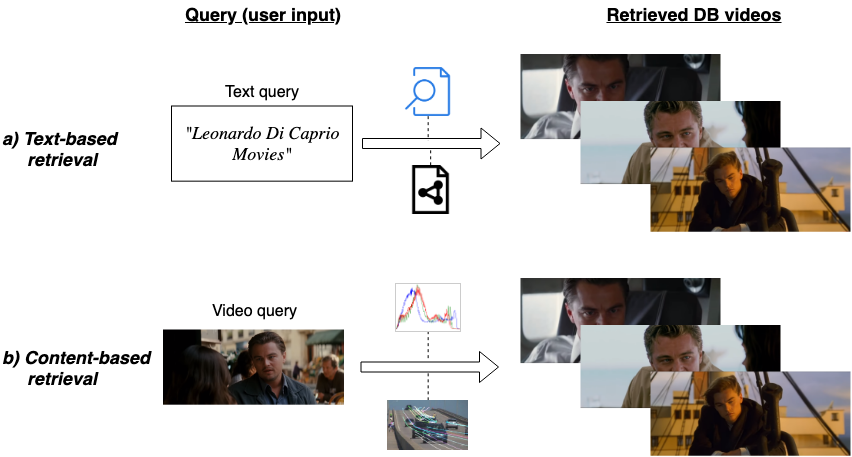
\includegraphics[width=\textwidth]{figures/content_text-retrieval_comparison.png}}
\caption{\label{fig:text_vs_content_retrieval}Illustrations of a text-based content-retrieval system \emph{(a)}, a content-based video retrieval system \emph{(b)}, and the project's desired CBVR system \emph{(c)}.}
\end{figure}

Content-based retrieval techniques quickly replaced text-based retrieval techniques towards the end of the 20th century by making use of the visual content to compute similarities between videos \cite{lai2015trajectory}. Instead of accepting a text string, the system takes a video as input to extract its visual contents, as shown in Figure \ref{fig:text_vs_content_retrieval}.\emph{b}. According to Petković et al. \cite{petkovic2000}, this visual content can be broken down into three different categories:
\begin{itemize}
    \item \textit{Raw data}, which corresponds to individual raw video frames and the video file's attributes such as the frame rate per seconds, the number of bits per pixel or the colour model used.
    \item \textit{Low-level visual content}  consists of the visual features that describe a video. This content includes colours, shapes, textures and motion. Low-level visual content can be extracted into static features such as histograms (see Section \ref{sec:color-based-features}) or dynamic features such as objects or motion (see Section \ref{sec:dynamic-features}) using a wide variety of existing techniques. Once the content has been extracted, it can be used to first compute similarities between videos \cite{lai2015trajectory} and later pattern match them.
    \item \textit{Semantic content} contains the high-level concepts that are present in a video. These high-level concepts can be described as objects or events using the features. To extract semantic content from a video, a grammar of rules for objects must be provided. An example of an object rule could be "if the shape is round, the colour is orange and the object is moving, then that object is a basketball".
\end{itemize}

In comparison to raw data, low-level visual content provides the most relevant visual information that can be extracted from a video for the purpose of a CBVR system. Semantic content extraction adds an additional layer of complexity compared to low-level visual content extraction as it requires domain knowledge and user interaction \cite{petkovic2000}. Therefore, this project will focus on using low-level visual content to extract information about the video and compute the similarities between the query video and database videos. It is important to note that this project's goal differs from classic CBVR systems where a list of videos is returned (see in Figure \ref{fig:text_vs_content_retrieval}.\emph{b}), as it must return a specific video that matches the most the query video. To improve the pattern matching accuracy phase, raw data (e.g. audio) and metadata (e.g. captions) may be used to improve the pattern matching accuracy \cite{patel2012}.\\

% ----------------------------------------------------

\subsection{Temporal Aspects of Videos}
\label{sec:temporal-aspect-videos}

\subsubsection{Temporal Structure of a Video}

The most important difference between content-based image retrieval and video retrieval lies within the temporal aspect of the video. Naturally, the temporal aspect of a video clip stores supplementary information about the content, including dynamic low-level visual content e.g. an object's motion, and semantic content e.g. actions and events. According to A. Araujo et al. \cite{araujo2017i2v}, a video's temporal structure can be subdivided into three units, as shown in Figure \ref{fig:temporal_structure}:
\begin{itemize}
    \item \textit{Frames} correspond to the smallest temporal unit of a video file. A single segment of a video is referred to as a frame. Frames are also used to describe the frame rate (the frequency at which consecutive stills appear on a screen every second) e.g. ``24 fps'' corresponds to a video made up of 24 stills per second.
    \item \textit{Shots} are grouped sequences of visually similar frames. They are usually described  in seconds.
    \item \textit{Scenes} are a collection of shots which are related based on the action and objects present in the shot, thus giving them a semantic aspect. The length of a scene 
    is generally calculated in minutes rather than seconds.
\end{itemize}

\begin{figure}[h]
\centerline{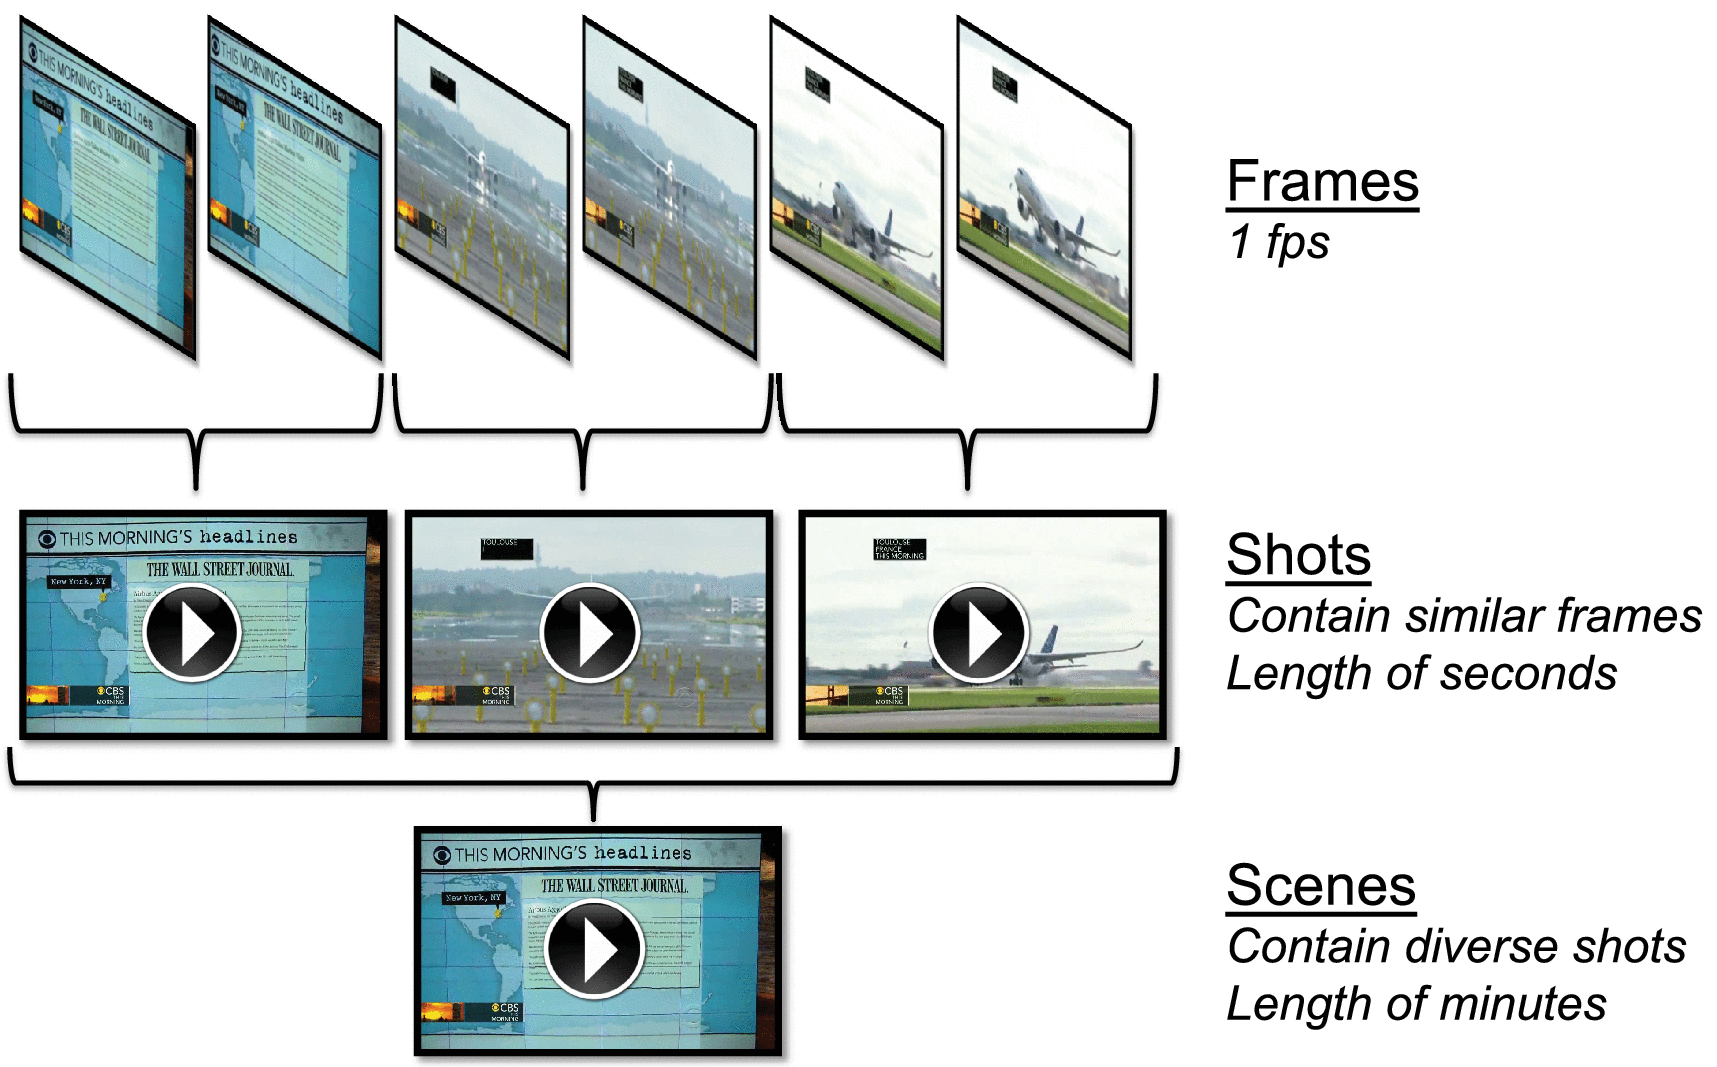
\includegraphics[width=0.75\textwidth]{figures/temporal_structure_videos.png}}
\caption{\label{fig:temporal_structure}Temporal structure of videos, including the different terms used to describe video temporal units. Figure courtesy of A. Araujo et al.}
\end{figure}

Because this project will explore possible solutions to create a CBVR system targeting databases of feature-length movies, a fourth video temporal structure category relevant to this project can be added to Araujo et al.'s initial list:
\begin{itemize}
    \item \textit{Movies} can be described as a large group of scenes that are used to tell a story. Movie durations commonly range from one to three hours.
\end{itemize}

\subsubsection{Challenges of Temporality}

Multiple challenges arise when dealing with CBVR systems in contrast to CBIR systems as the videos' temporal aspect adds a new dimension of complexity when extracting visual information. While the low-level visual content describing images remains mostly the same for videos (see Section ref-section), some new information that did not exist in images can be extracted, such motion. As mentioned previously, videos are a made up of frames, which make up shots when a combination of similar frames are played in succession. This means that videos carry information about motion, such as the trajectory of objects. This introduces unique challenges to the algorithms used to extract motion.\\

Because videos are made up of numerous stills, usually around 24 frames per second \cite{brownlow1980silentfilm}, two consecutive frames are near-identical. The pixels describing an object in one frame will remain the same in the next frame, except for the edge pixels perpendicular to the motion's trajectory \cite{bradski2008opencv}.\\

Figure \ref{fig:forrest_gump_frames} shows six frames from Forrest Gump's famous running shot, which lasts 44 seconds, making up a total of 1056 frames. Each frame in the figure was captured with 10-second intervals, meaning 240 frames separate each still. In the first three frames, the group of people running in the background barely moves in the space of 20 seconds. The pixels that describe the group in the shot remain mostly unchanged for all of the frames between the 3 samples, equivalent to 480 frames, with a few additional pixels describing the group as it advances towards the camera. The same can be said about the red cap in the last two frames. Most of the pixels making up the cap in the fifth frame remain the same in the sixth frame. This example perfectly betrays the reason why analysing a video frame by frame would be extremely inefficient when it comes to CBVR. Due to the similarities between consecutive frames, these should be aggregated \cite{araujo2017i2v} to describe a shot by using a selection of frames, such as taking the six frames in Figure \ref{fig:forrest_gump_frames} to describe the entire 44 seconds of video, rather than keeping the original 1056 frames to describe it.

\begin{figure}[h]
\centerline{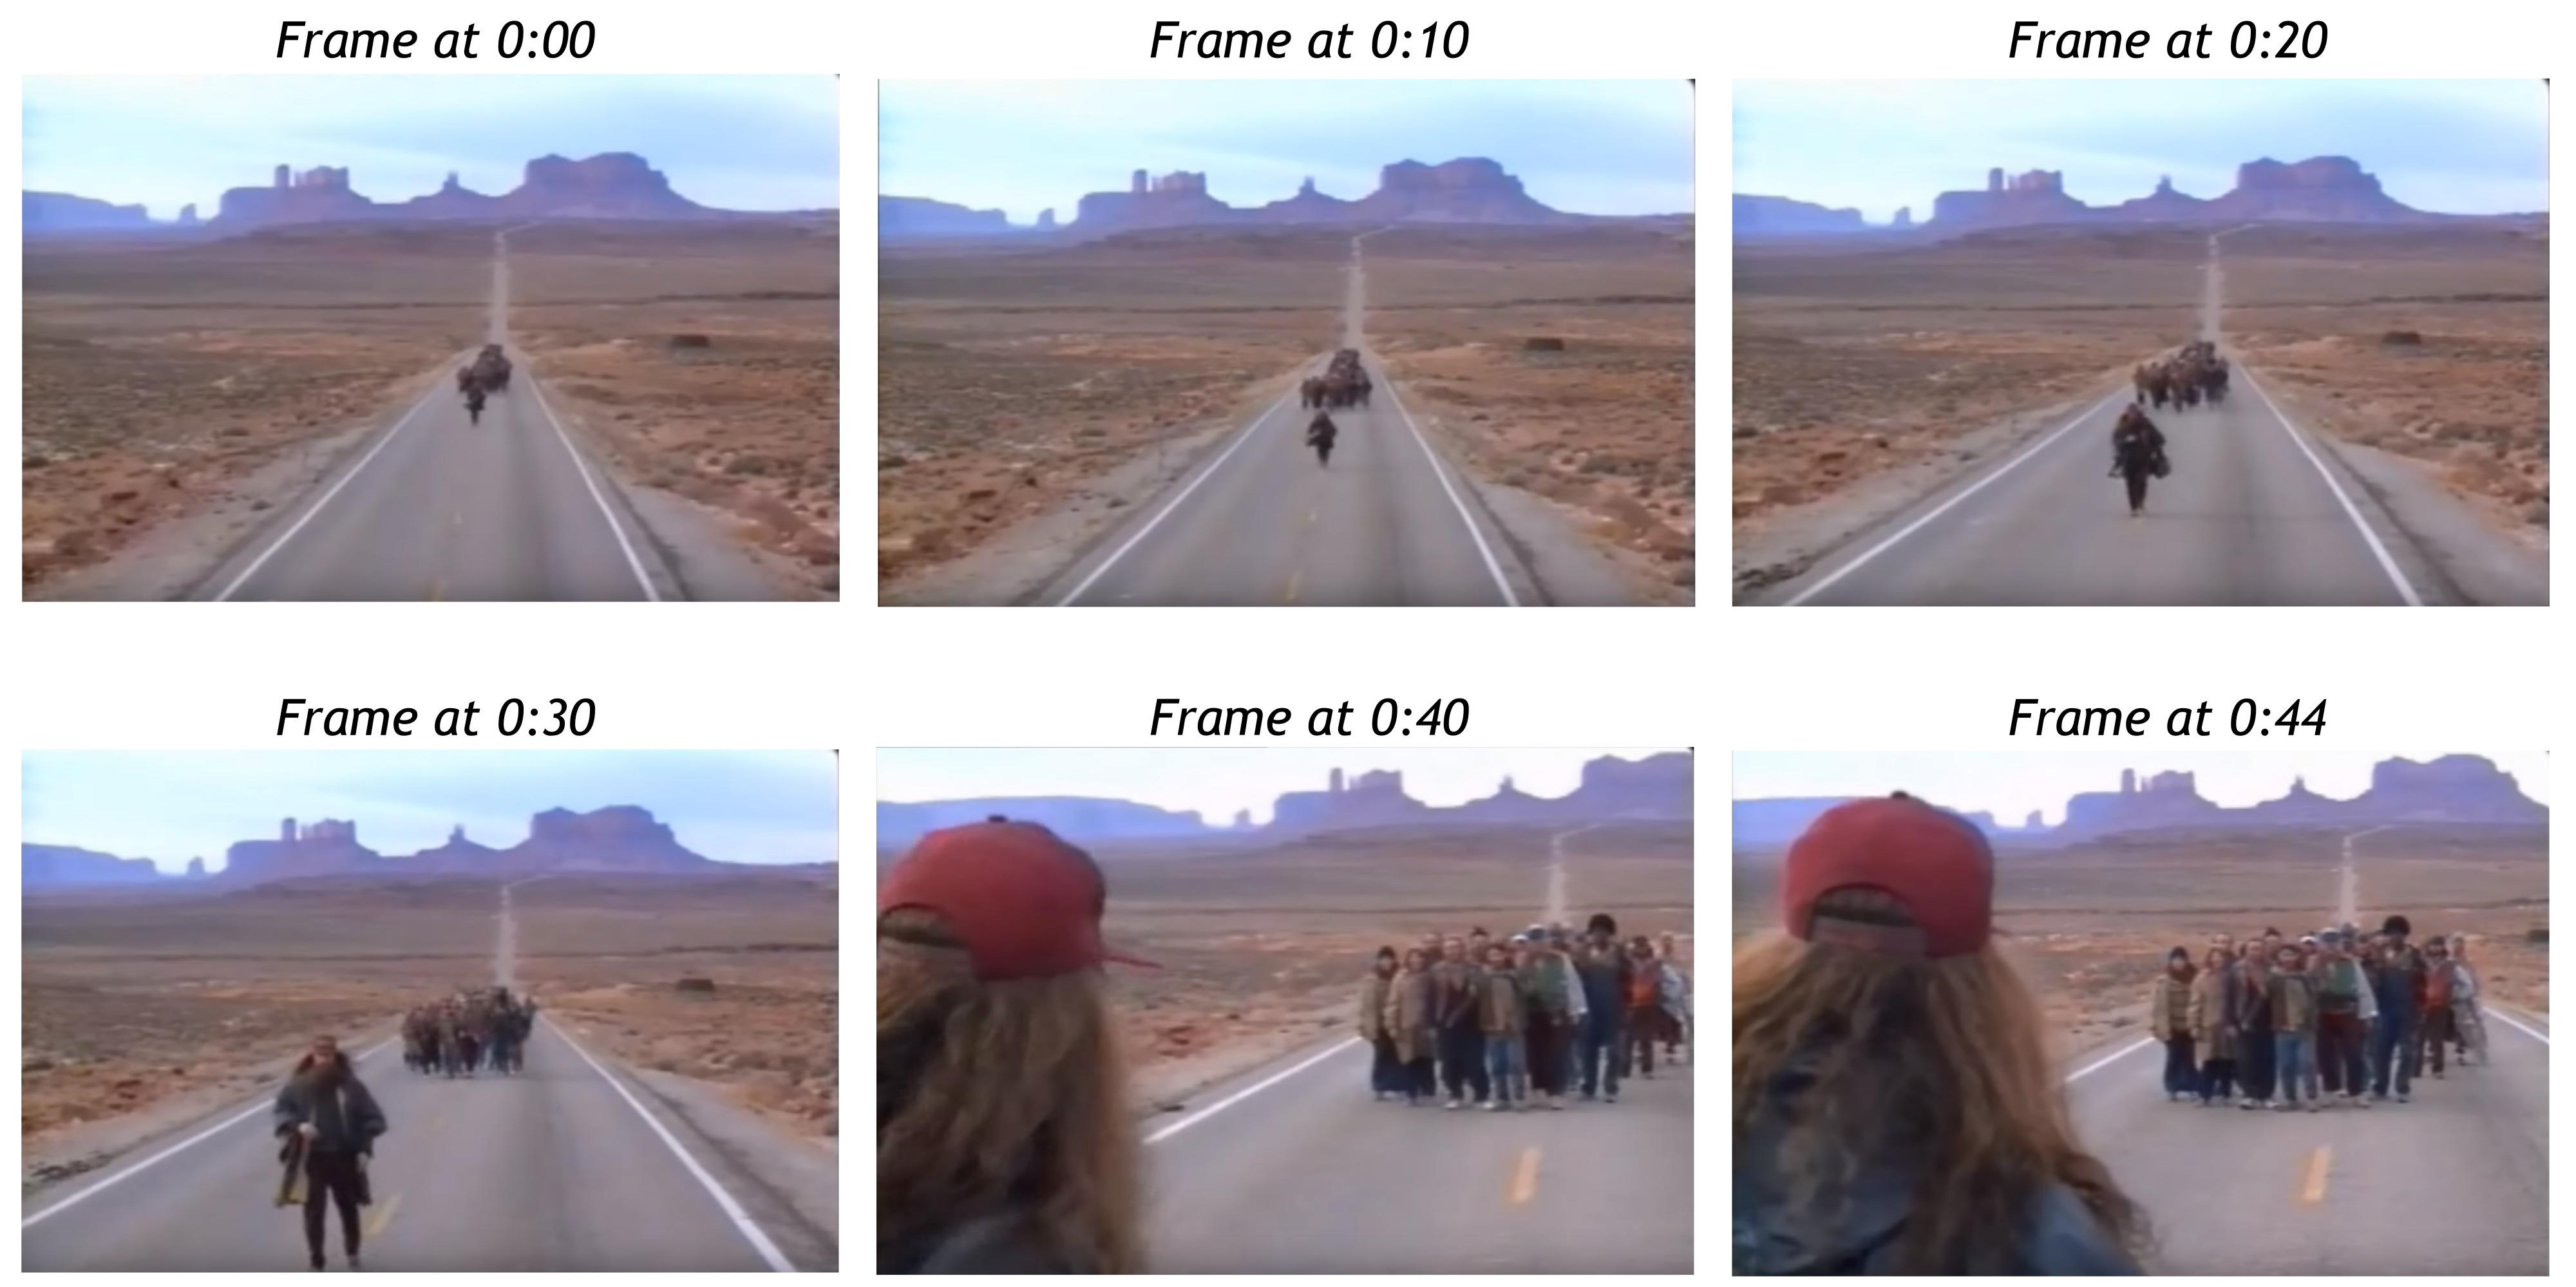
\includegraphics[width=\textwidth]{figures/forrest_gump_shot.jpg}}
\caption{\label{fig:forrest_gump_frames}Frames from the famous running scene in Forrest Gump extracted at intervals of 10 seconds. Video frames courtesy of \textit{``Forrest Gump long run scene"} YouTube video available online: \url{https://youtu.be/QgnJ8GpsBG8?t=325}.}
\end{figure}

\begin{comment}
    On top project aim mobile device using a database of feature-length movies.\\
    \cite{araujo2017i2v}One of the problems regarding video retrieval is the temporal aspect of the data. A solution to overcome the temporal aspect of the data is to aggregate each video into a compact signature to allow quicker and more efficient matching (when matching the query video to a video in the database).\\ 
    temporal aggregation problem of videos compared to images
\end{comment}

% ----------------------------------------------------

\subsection{CBVR for Mobile Devices}

The aforementioned project aim is for the system to work on mobile devices for two reasons. The first reason, as shown in Figure \ref{fig:wireframe} is to allow users to directly use their mobile phone to record the query video by pointing their camera to a screen displaying a movie, which will in turn tell them which movie is being played. Additional information retrieved from IMDb\footnote{Internet Movie Database}, such as cast, crew, ratings, runtime and synopsis could also be displayed. The second reason is the popularity of mobile devices, which may be due to the improvements made on mobile phones' processing power, allowing more tasks to be carried out through this medium. However, such a system on a mobile device causes many problems regarding the query video recording method and the computational power available on mobile devices.\\

\begin{figure}[h]
\centerline{\includegraphics[width=1.15\textwidth]{figures/system_wireframe.png}}
\caption{\label{fig:wireframe}Wireframe showing the basic high-level concept of the system.}
\end{figure}

\subsubsection{Query Video Quality}

Large visual differences are caused between the query clip and the actual clip stored in the database due to the capture conditions \cite{liu2014mobilevideosearch} \cite{wang2016actionregonition} such as:
\begin{itemize}
    \item Undesired camera movements due to unstable recording e.g. unstable recording, hand shaking.
    \item Low-quality recording due to poor user recording e.g. scaling and rotation, and due to the environment conditions e.g. lighting, reflections, blurring.
    \item Video noise because of the camera sensor.
    \item Decoding artefacts causes by various file compression.
\end{itemize}

These low-quality conditions add difficulty to the pattern matching phase where the similarities between the query video and database videos have to be computed. Indeed, if the query video is very different to the actual video, then the noisy elements of the video query must filtered out. For example, if the recorded video is shaky, then this shaking motion has to be pruned before analysing the recorded clip's motion. However, processing power must be used from the actual visual content extraction and pattern matching phases to be used for video noise filtering.

\subsubsection{User Experience}

According to Liu et al. \cite{liu2014mobilevideosearch}, the majority of mobile device users expect a polished product with quick video query and instant or progressive results, meaning that the searching algorithms must be efficient. However, one of the downsides of mobile devices is the computation power constraints. Despite the improvements of mobile processors, desktop devices still remain more powerful than mobile ones. A solution that Liu et al. suggest is to retrieve the low-level visual content locally on the mobile device, and send the query to a server where the pattern matching will take place \cite{liu2014mobilevideosearch}. This allows heavy computations to be off-loaded from the mobile device. Once a match is found, the result is returned to the user on his mobile device. A downside to this approach is the new constraint on network bandwidth rather than computational power.

\begin{comment}
    % todo - spread in sections above
    \subsubsection{Computational efficiency and database size}
    
    At the early stages of the development phase of the project, the database of videos for the system will be made up of shots only, lasting on average ten seconds. Longer videos will be used progressively based on the system's progress with shorter videos.\\
    mention \cite{hanjalic1999moviesegmentation}
    
    \cite{wang2016actionregonition}
    A challenge also lies within the computational power needed to process all the data in a database efficiently.\\
\end{comment}


%%%%%%%%%%%%%%%%%%%%%%%%%%%%%%%%%%%%%%%%%%%%%%%%%%%%%%%%%%%%%%%%%%%%%%%%%%%%%%%%%%
% 2 - VISUAL CONTENT EXTRACTION FOR PATTERN MATCHING VIDEOS
%%%%%%%%%%%%%%%%%%%%%%%%%%%%%%%%%%%%%%%%%%%%%%%%%%%%%%%%%%%%%%%%%%%%%%%%%%%%%%%%%%
\section{Visual Content Extraction for Pattern Matching Videos}
\label{sec:visual-content-extraction}

Extracting the visual content from a video allows this content to be used to describe videos and compute similarities between them. This visual content is extracted from the aforementioned low-level visual content (see Section \ref{sec:cbvr-methods}) \cite{petkovic2000} and stored in the form features, also referred to as visual descriptors. The term ``features'' is very broad and can be used to describe many different visual aspects in an image or in a video, ranging from colours, shapes and textures to points, edges, objects and motion.\\

These features can be divided into two categories: static features and dynamic features \cite{petkovic2000}. This section will first survey examples of static visual descriptors and methods to extract them from videos, and will then focus on examples and methods of extracting dynamic visual descriptors from videos.

% ----------------------------------------------------

\subsection{Static Features}

Methods to extract static features operate on stills, which can correspond to individual video frames, thumbnails or key frames. This means that traditional image techniques can be applied on those stills \cite{hu2011survey}. They are organised in three different categories: colour-based features, texture-based features and shape-based features.

\subsubsection{Colour-based Features}
\label{sec:color-based-features}

The main colour-based features model are colour histograms. In general, a histogram consists of counts of some underlying data that is organised into predetermined bins to a statistical representation of the distribution of that data. Figure \ref{fig:histogram-general-example} depicts an example of a histogram where a collection of points is organised into specific ore-defined bins based on their location relative to a vertical grid.

\begin{figure}[h]
\centerline{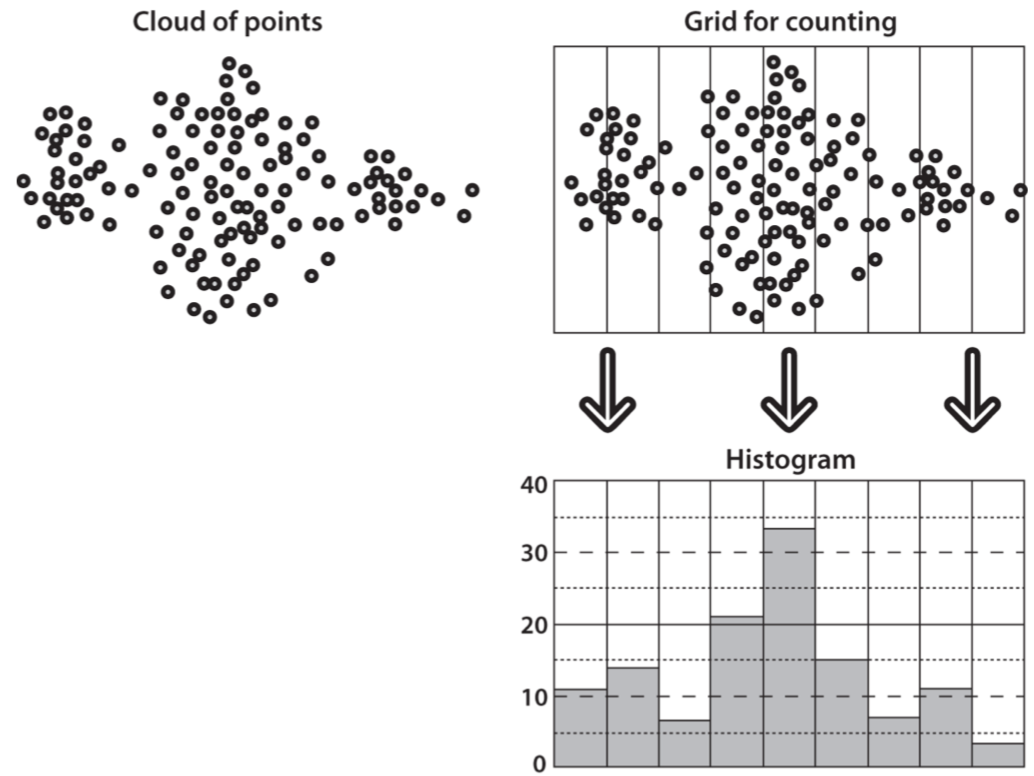
\includegraphics[width=0.70\textwidth]{figures/histogram_general_example.png}}
\caption{\label{fig:histogram-general-example}Example of a histogram counting the location of points relative to a vertical grid. Image courtesy of Bradski and Kaehler.}
\end{figure}

In the case of a colour histogram, the underlying data that the histogram is trying to represent is the distribution of the colour pixels throughout an image or a video frame. Different kinds of colour histograms exist as they depend on the chosen colour space, which include RGB\footnote{Red Green Blue}, HSV\footnote{Hue Saturation Value}, HSL\footnote{Hue Saturation Light} or YPbPr colour spaces to name a few. These may vary based on the applications of the colour histograms.\\

Typically, for a RGB colour histogram, 256 bins are used to accurately represent all the possible values that the pixels can take (ranging from 0 to 255) for each of the three RGB channels, which are then plotted as three individual graphs. Choosing the right range for the histogram's bins is crucial to represented the distribution efficiently. If the range of pixels that defined the bins is wider, meaning there are less overall bins, then the histogram's distribution would be too coarse-grained and the general structure of the histogram would be lost, as pointed out by the left half of Figure \ref{fig:histogram-bin-size}. On the other hand, if the range of the bins is too narrow, meaning there are more overall bins, then the histogram's distribution would not be represented accurately and there would be many spiky cells, as betrayed in the right half of Figure \ref{fig:histogram-bin-size} \cite{bradski2008opencv}.

\begin{figure}[h]
\centerline{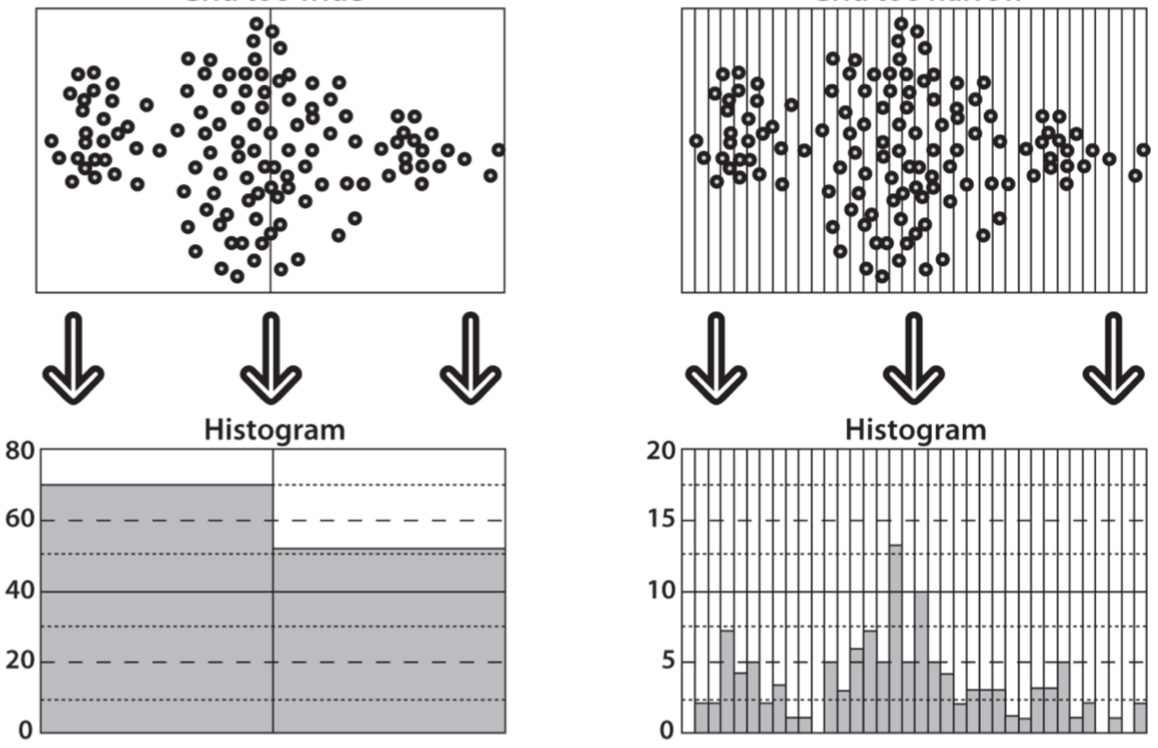
\includegraphics[width=0.80\textwidth]{figures/histogram_bin_size.png}}
\caption{\label{fig:histogram-bin-size}If the range of the bins is too large, then the distribution is coarse (left). If the range of the bins is too small, then the distribution is not accurately represented and spikes cells appear (right). Image courtesy of Bradski and Kaehler.}
\end{figure}

One of the inaccuracies with colour histograms lies within the scope of the distribution. If the histogram represents the global distribution of all the pixels in the still, then two images might have very similar histograms \cite{petkovic2000}. For example, a histogram containing 60\% white pixels and 40\% blue pixels could either describe both a blue sky with white clouds, or a snowy landscape with a blue sky. Despite both histograms being good colour-based features, the actual result is still poor when it will be used for matching the histograms. A solution consists in segmenting the still into multiple local images, and extract the local colour-based features for each segment. For example, the still could be partitioned into a 5x5 grid, and a colour histogram could then be computed for each grid \cite{yan2007review}. This would enable colour-based features to represent specific regions of the still rather than globally describing an image. However, the same problem mentioned earlier could occur if the still is segmented into too many regions, causing the overall histogram to be coarse.\\

Other types of colour-based features can be extracted from images and videos such as colour moments, colour correlograms \cite{huang1997correlograms} and Gaussian models. However, colour-based features have their limitations as they cannot describe textures and shapes, rendering them inefficient in certain applications \cite{hu2011survey}.

\subsubsection{Texture-based Features}

Texture-based features are often used in parallel with colour-based features. The aforesaid problem where two different objects might share a similar histogram e.g. green tree leaves and green grass, can be solved by using texture-based features to differentiate them. These can be differentiated by using a variety of features such as Tamura features, which extract information including coarseness, contrast, and directionality of the objects \cite{amir2003ibm}. 

\subsubsection{Shape-based Features}

Shape-based features are used to describe the overall shape of objects present in the image. The most common approach consists in computing a EHD\footnote{Edge Histogram Descriptor}, which consists in detecting the edges present in the image (see Section edges) and then plot their spatial distribution in an histogram by counting the number of pixels for each edge \cite{hauptmann2004informedia}. The same image segmentation technique can be used to localise the EHD. These shape-based features have many applications, but are harder to extract and require more computing power than colour-based features and texture-based features.

% ----------------------------------------------------

\subsection{Dynamic Features}
\label{sec:dynamic-features}

In contrast to static features, which can be extracted from individual video frames, dynamic features require the continuity between consecutive frames to extract relevant visual descriptors, making use of the temporal aspect of the video mentioned in section \ref{sec:temporal-aspect-videos}). These features can be divided into two subcategories: object features and motion features. However, before reviewing the techniques used to extract these features, it is important to specify what defines a good visual feature.

\subsubsection{Corner Detection}

Figure \ref{fig:monaco_palace_features} shows an image with coloured windows used to make the difference between poor and good potential features that could be used for object and motion features:
\begin{itemize}
	\item \textit{Flat surfaces} are portrayed in blue in Figure \ref{fig:monaco_palace_features}. These blue windows are spread over large areas of the image, meaning it is difficult to find their specific location. Moving the blue window along the image in any direction will result in the same visual content being represented in the window. Therefore, these flat regions are the worst structures as they do not contain any useful information.
	\item \textit{Edges} are characterised in green in Figure \ref{fig:monaco_palace_features}. These are more informative than flat surfaces as they can be more accurately localised, but pinpointing an exact location is still hard as the patch can be moved in the direction parallel to the edge's. Moving the green window along the edge will again result in the same visual content being represented in the window. Edges are efficient to detect object boundaries, but not for tracking specific points.
	\item \textit{Corner} are characterised in red in Figure \ref{fig:monaco_palace_features}. These are the most descriptive points as they are often unique and can be precisely located in an image. Moving the red window in any direction will cause it to look different. Corners are therefore the ideal candidate for features used in object matching and tracking.
\end{itemize}

\begin{figure}[h] 
\centerline{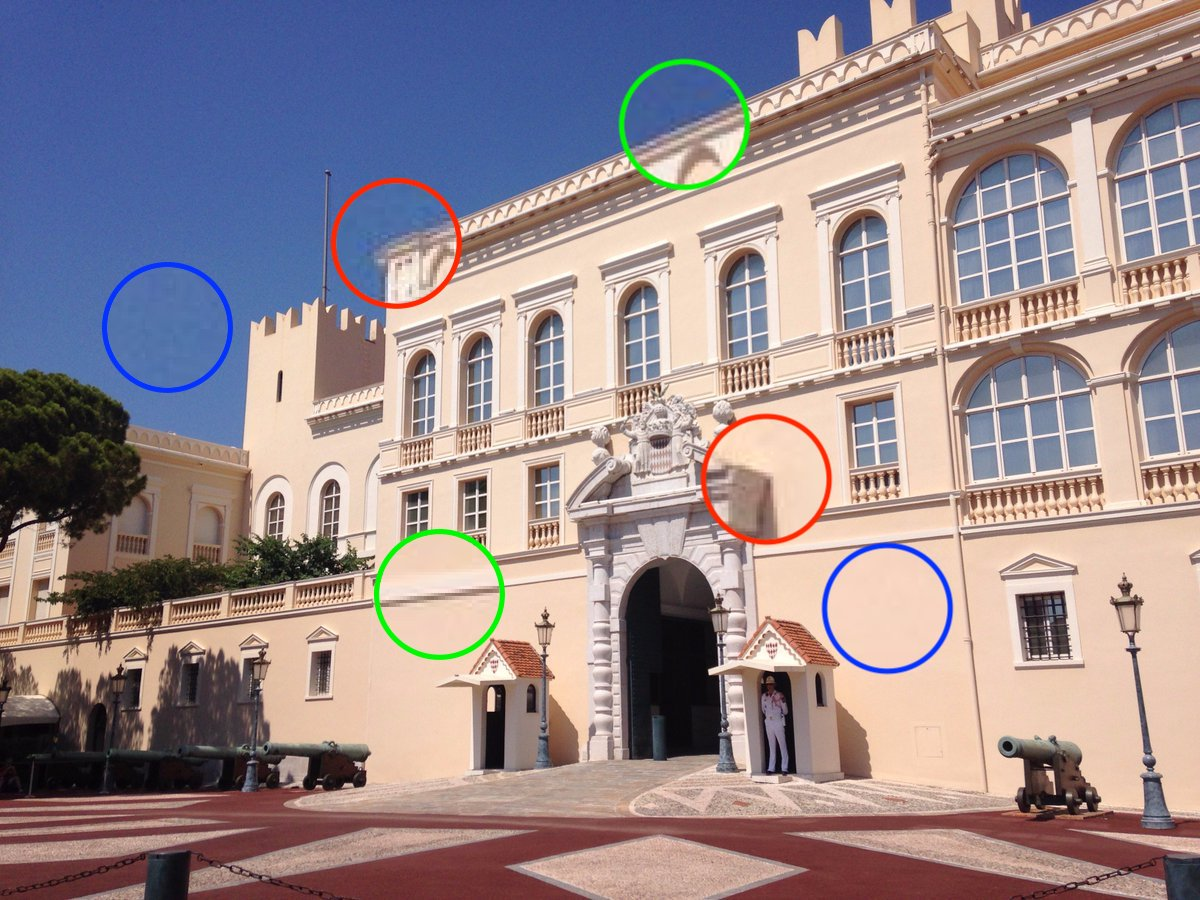
\includegraphics[width=0.75\textwidth]{figures/monaco_palace_features.jpg}}
\caption{\label{fig:monaco_palace_features}An image of the Palace of Monaco with coloured windows representing poor features in blue (flat), edges in green, and good features in red (corners).}
\end{figure}

Once expressive and unique descriptors like corners are detected, they can be used to extract object features and motion features, and to compute similarities between the query video and the videos in the database.\\

Many different techniques exist to find robust features and interest points: Harris Corner Detection, SIFT, SURF.

\begin{comment}
    detect edges and then use that to detect corners
\end{comment}

\subsubsection{Object Features}

Object features correspond to objects that are detected using the colour, texture and size of image regions. Some of the most common objects usually detected in videos are faces, as many CBVR systems use them to compute similarities between videos \cite{sivic2005face}. However, extracting object features is time-consuming and expensive in terms of required processing power, which is why CBVR algorithms either focus on detecting specific sets of objects rather than general objects that may be present in a scene, or on static features.

\subsubsection{Motion Features}

camera-based motion features

object-based motion features

Example algorithms: optical flow (Dense Optical Flow, Farneback Polynomial Expression Algorithms, Lucas-Kanade Algorithm.
Can calculate optical flow to prune camera movement caused by unstable recording e.g. hand shaking movement \cite{wang2016actionregonition}.


%%%%%%%%%%%%%%%%%%%%%%%%%%%%%%%%%%%%%%%%%%%%%%%%%%%%%%%%%%%%%%%%%%%%%%%%%%%%%%%%%%
% 3 - LEARNING MODELS FOR FEATURE MATCHING
%%%%%%%%%%%%%%%%%%%%%%%%%%%%%%%%%%%%%%%%%%%%%%%%%%%%%%%%%%%%%%%%%%%%%%%%%%%%%%%%%%
\section{Learning Models for Classification}

Multiple techniques exist to retrieve a video's visual information to later compare it to the visual information stored in the database.
Retrace evolution of pattern matching methods: BoW to CNN (and before? --> find surveys)

% ----------------------------------------------------

\subsection{Bag-of-Visual-Words}

\subsubsection{BoW}
BoW for documents

\subsubsection{BoVW}

BoVW

TODO:
\begin{itemize}
    \item Explain how Bag-of-Words model works
    \item H. Wang's implementation of BoW histogram \cite{wang2016actionregonition}
    \item State that Fisher Vectors are an improvement on BoW
\end{itemize}

\subsubsection{Histogram Comparison}

chi-square
alternative chi-square
intersection
bhattacharyya

% ----------------------------------------------------

\subsection{Deep Learning}

\subsubsection{Classical Neural Networks}

nn

\subsubsection{Convolutional Neural Networks}

cnn


%%%%%%%%%%%%%%%%%%%%%%%%%%%%%%%%%%%%%%%%%%%%%%%%%%%%%%%%%%%%%%%%%%%%%%%%%%%%%%%%%%
% 4 - STRUCTURAL MOVIE PRE-PROCESSING
%%%%%%%%%%%%%%%%%%%%%%%%%%%%%%%%%%%%%%%%%%%%%%%%%%%%%%%%%%%%%%%%%%%%%%%%%%%%%%%%%%
\section{Structural Movie Pre-Processing}

The database of videos can be pre-processed to optimise the visual content extraction and pattern matching phases. As stated in Section \ref{sec:temporal-aspect-videos} on the temporal aspects of videos, movies can be defined as a logically ordered collection of scenes, which may contain different shots, all made up of individual frames. Pre-processing the database of movies by segmenting it into a list of shots and representing each shot with a single key frame is a profitable solution that will exponentially improve a CBVR system's efficiency. However, a limit must be set on the amount of data that is segmented to balance the efficiency and the accuracy of the CBVR system.

% ----------------------------------------------------

\subsection{Temporal Movie Segmentation}

The frames that make up a shot usually show strong content correlation. This means that features extracted from one frame will be extremely similar in another frame from the same shot. Detecting shot boundaries would allow the movie to be segmented and organised by shots, as depicted in Figure \ref{fig:shot_boundary_detection}. These boundaries are defined by the type of transition between two different shots, which can either be defined as a quick cut when the transition is direct, or as gradual when it is a dissolve or fade in/out transition \cite{yuan2007shotboundary}, as shown in Figure \ref{fig:video_transitions}.

\begin{figure}[h] 
\centerline{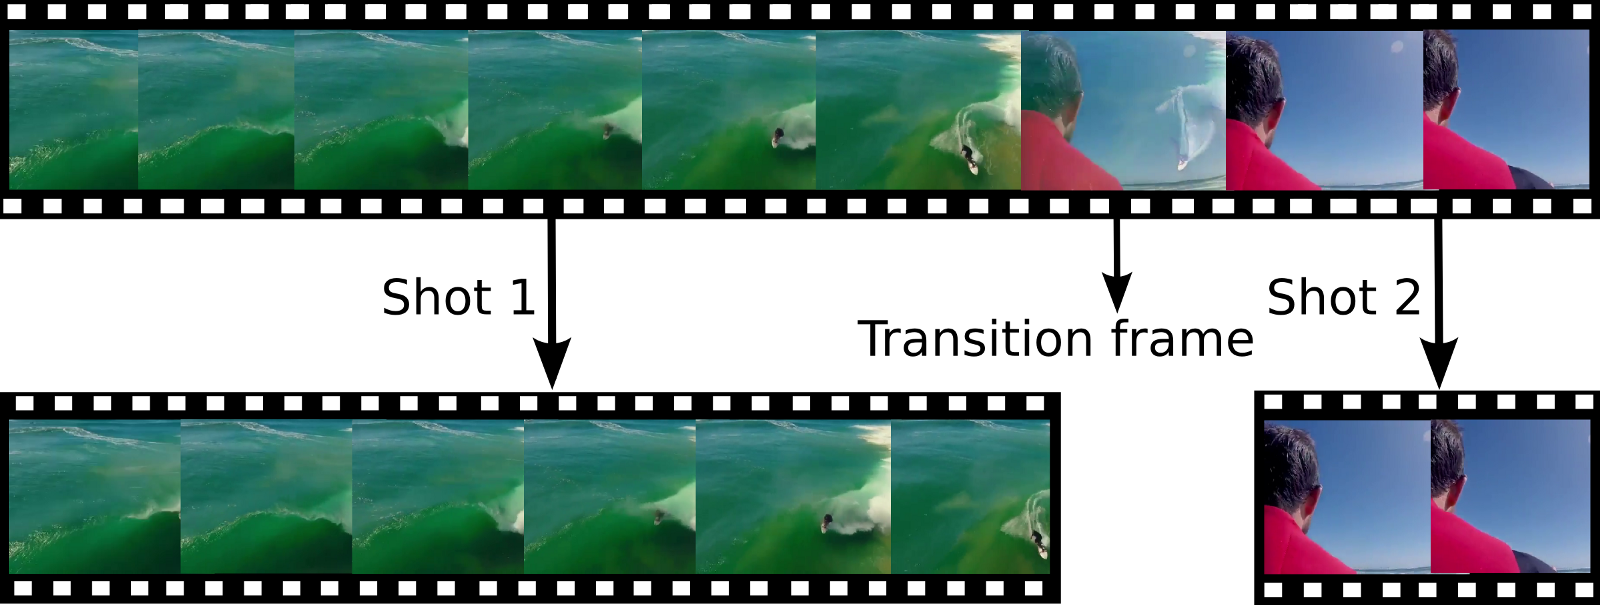
\includegraphics[width=0.75\textwidth]{figures/shot_boundary_detection.png}}
\caption{\label{fig:shot_boundary_detection}Shot boundary detection example of a video made up of two shots with a gradual transition. Figure courtesy of Michael Gygli available online at: \url{https://medium.com/gifs-ai/\_ridiculously-fast-shot-boundary-detection-with-fully-convoluti\_onal-neural-networks-da9d8c73e86c}}
\end{figure}

\begin{figure}[h] 
\centerline{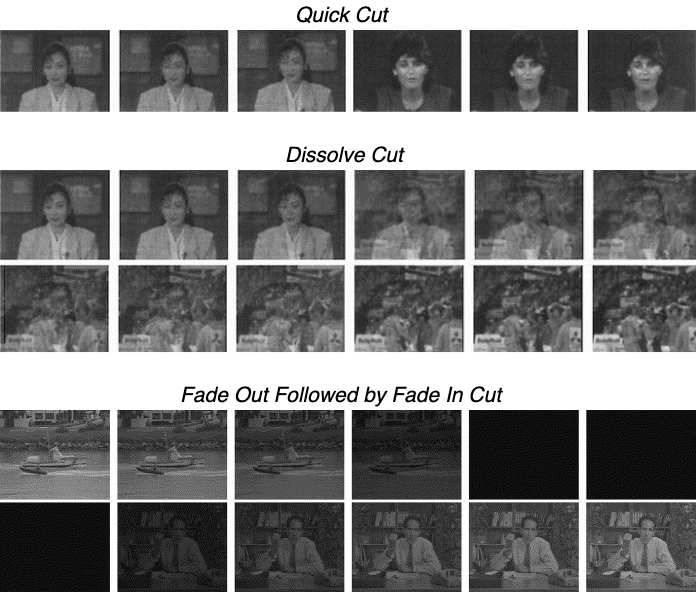
\includegraphics[width=0.75\textwidth]{figures/video_transitions.png}}
\caption{\label{fig:video_transitions}. Visual examples of a quick cut, a dissolve cut and a fading cut. Frames courtesy of (Koprinska, Carrato, 2001) ``Temporal video segmentation: A survey'' available online at: \url{https://www.sciencedirect.com/science/article/pii/S0923596500000114}}
\end{figure}

Temporal video segmentation requires three steps:
\begin{enumerate}
    \item feature extraction
    \item similarity measurements
    \item shot boundary detection
\end{enumerate}

\subsubsection{Feature Extraction}
The first step in video segmentation consists in extracting features. These features include all the diverse types mentioned in Section \ref{sec:visual-content-extraction}, ranging from static features such as colour-based features (e.g. colour histograms) to dynamic features such as corner points and SIFT\footnote{Scale Invariant Feature Transform}. Although colour histograms are simple to compute and work well with most shots as long as there is at most minor camera movement, they are inefficient when the shots contain major camera movements. For example, if in the shot the camera moves from the inside a house towards the outside by going through the window, the frames retrieved from the beginning of the shot will be extremely different to frames from the end of the shot.\\

Dynamic features are therefore more efficient for shot boundary detection than histograms due to their robustness. On the one hand, edge features are more vigorous than histograms when dealing with major camera movement and can handle changes in luminosity. On the other hand, corner and motion features can additionally handle camera motion and the impact of objects in the shot such rapid motion e.g. people walking in front of the camera. However, these dynamic features are much more complicated to extract and do not always outperform colour histograms. Due to their simplicity, colour histograms remain the most common feature extraction technique for shot boundary detection.\\

\subsubsection{Similarity Measurements}
The second step in video segmentation is to use these extracted features to compute the similarities between frames. Many metrics exist to compute the similarities between two the extracted features. The most basic method consists in computing the Euclidean distance between features. More advanced methods can be used based on the type of feature that was extracted. For instance, histogram intersection and chi-square similarity can be used to compute the relationship between colour histograms. During the 2006 TRECVID conference, \cite[p.2]{hoi2006trecvid06} used gray scale histograms for their extracted features and calculated the colour differences between frames using the EMD\footnote{Earth Mover's Distance}. EMD is used to calculate the distance between two probability distributions, which are represented by the two histograms that represent each frame in \cite{hoi2006trecvid06}'s case. These similarities can be measured using two techniques.\\

The first technique rests on using pairs of frames to compute the similarities between them. The similarities between two consecutive frames $I_1$ and $I_2$ are compared, before comparing the pair of frames $I_2$ and $I_3$, and so on and so forth until frames $I_{n-1}$ and $I_n$ are compared. This straightforward technique easily detects rough changes between the visual content in a shot, such as quick cuts between two shots, but is more susceptible to noise and disturbance.\\

The second technique is the window-based similarity measure, that measures the similarities between multiple frames specified within a range. This helps counter the effects of noise and disturbances captured by the pair-based approach but is more expensive to compute, therefore less used.

\subsubsection{Detection}
The final step in segmenting a video is the detection of the frames to cut, which is achieved by using the measured similarities between the frames. Two methods exist for this step: a threshold-based approach and a statistical learning-based approach.\\

The threshold-based approach compares the measured similarities between a pair of frames with a threshold. Whenever the similarity measure is smaller than the threshold, a shot boundary is detected and the shot can be cut. Figure \ref{fig:shot_boundary_detection_threshold} betrays an example of a threshold-based approach for different types of transitions, with a correct detection (\emph{A}), a missed detection (\emph{B}) and a misinterpreted detection (\emph{C}).\\

\begin{figure}[h] 
\centerline{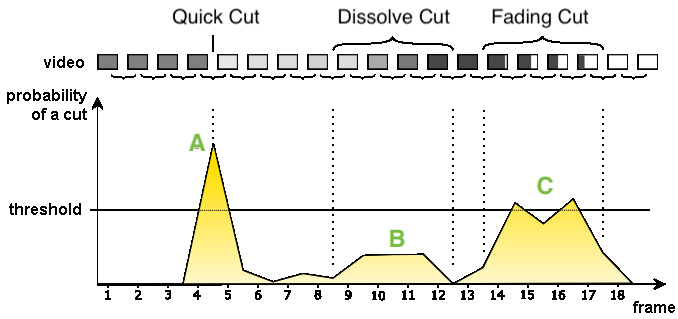
\includegraphics[width=0.75\textwidth]{figures/shot_boundary_detection_threshold.png}}
\caption{\label{fig:shot_boundary_detection_threshold}Threshold-based approach for shot boundary detection. In this example, the shot boundary is detected at \emph{A}, it is missed at \emph{B}, and it is misinterpreted at \emph{C} as two cuts rather than a single one.}
\end{figure}

Either global thresholds, adaptive thresholds, or combinations of both can be used:
\begin{itemize}
    \item \textit{Global thresholds} are set empirically and predefined for the entire video. They are therefore inefficient when trying to detect local variations as these are not integrated into the initial global threshold calculations.
    \item \textit{Adaptive thresholds} are local thresholds that are continuously calculated for windows of frames. As the window slides across the video, the threshold is re-estimated accordingly to account for local variations. These are more accurate than global thresholds but are harder to estimate and require some knowledge about the video to set variables such as the window's size.
    \item \textit{Combination of global and adaptive thresholds} are adaptive thresholds that take into account the values of global thresholds when estimating the frames within the window. Different thresholds can be determined for different types of transitions such as cut and dissolve transitions. However, these add additional complexity to the threshold estimation.
\end{itemize}

The statistical learning-based approach is two-class classification task where each frame is classified either as a ``shot change`` or as a ``no shot change`` based on the extracted features and the similarity measurements between those features. Two types of classifiers can be used for this approach:
\begin{itemize}
    \item \textit{Supervised learning-based classifiers}, such as the SVM\footnote{Support Vector Machine} and Adaboost. These supervised learning approaches have multiple advantages compared to threshold-based approaches as they do not require thresholds to be set and many different types of features can be combined in the feature extraction step to increase the classifier's accuracy. However, this approach requires more expertise as the classifier relies on a well-trained data set to remain accurate.
    \item \textit{Unsupervised learning-based classifiers} are divided into frame similarity-based and frame-based algorithms. \textit{Frame similarity-based classifiers} groups the similarity measurements between a pair of frames into two clusters. The first cluster holds the similarity measurements with low values, which correspond to the ``shot change'' class, while the second cluster holds the similarity measurements with high values, which correspond to the ``no shot change'' class. Alternatively, \textit{frame-based classifiers} consider each shot as a cluster of frames with similar features. The advantage of unsupervised learning-based classifiers over supervised ones is that no training is required, but the logical temporal order of the shots in scenes is not preserved.
\end{itemize}

All the aforementioned techniques in this section that are used in the three steps required in the process of segmenting a video can be applied to feature-length movies but require some improvements to work efficiently with these large videos. For instance, \cite{hanjalic1999moviesegmentation} suggests considering the semantic aspects of movies, since people relate to the story, such as a marking dialogue, when they remember a movie.

% ----------------------------------------------------

\subsection{Key Frame and Thumbnail Extraction}

\subsubsection{Key Frames}

Y. S. Heo et al. \cite{heo2016colortransfer} suggests only considering key frames in videos to operate on. These key frames would be used for the feature extraction, database pre-processing and pattern matching phases. Key frames are determined based on the difference between two consecutive frames using the histogram chi-square distribution approach (See Equation \ref{eq:chisquare}).\\

\cite{heo2016colortransfer}
This approach only considers key frames from the query video clip. Key frames are determined based on the difference between two consecutive frames using the histogram chi-square distribution approach (See Equation \ref{eq:chisquare}).\\

TODO:
\begin{itemize}
    \item Explain histogram chi square distribution technique.
    \item When the amount of differences $\theta$ between two frames exceeds a threshold, usually set at the empirical value $\theta = 0.005$, then the current frame is set as a key frame.
\end{itemize}

\begingroup \Large \begin{equation} \label{eq:chisquare}
    C(h^{t-1}, h^{t}) = \sum_{i=0}^{255} \frac{(h_{i}^{t-1} - h_{i}^{t})^2}{h_{i}^{t-1} + h_{i}^{t}}
\end{equation} \endgroup \\

To illustrate the advantage of using key frames, let's use a 3-seconds long shot recorded at 30 fps\footnote{Frames Per Second} of a ball rolling on the ground, which would consist of a total of 90 frames. Analysing all the frames individually as stills would be highly inefficient. However, selecting key frames to work on, as depicted in Figure \ref{fig:rolling_ball} where a single frame is chosen for each second, would means that 3 key frames can be used for feature extraction and pattern matching instead of using all of the 90 frames that make up the video.\\

\begin{figure}[h]
\centerline{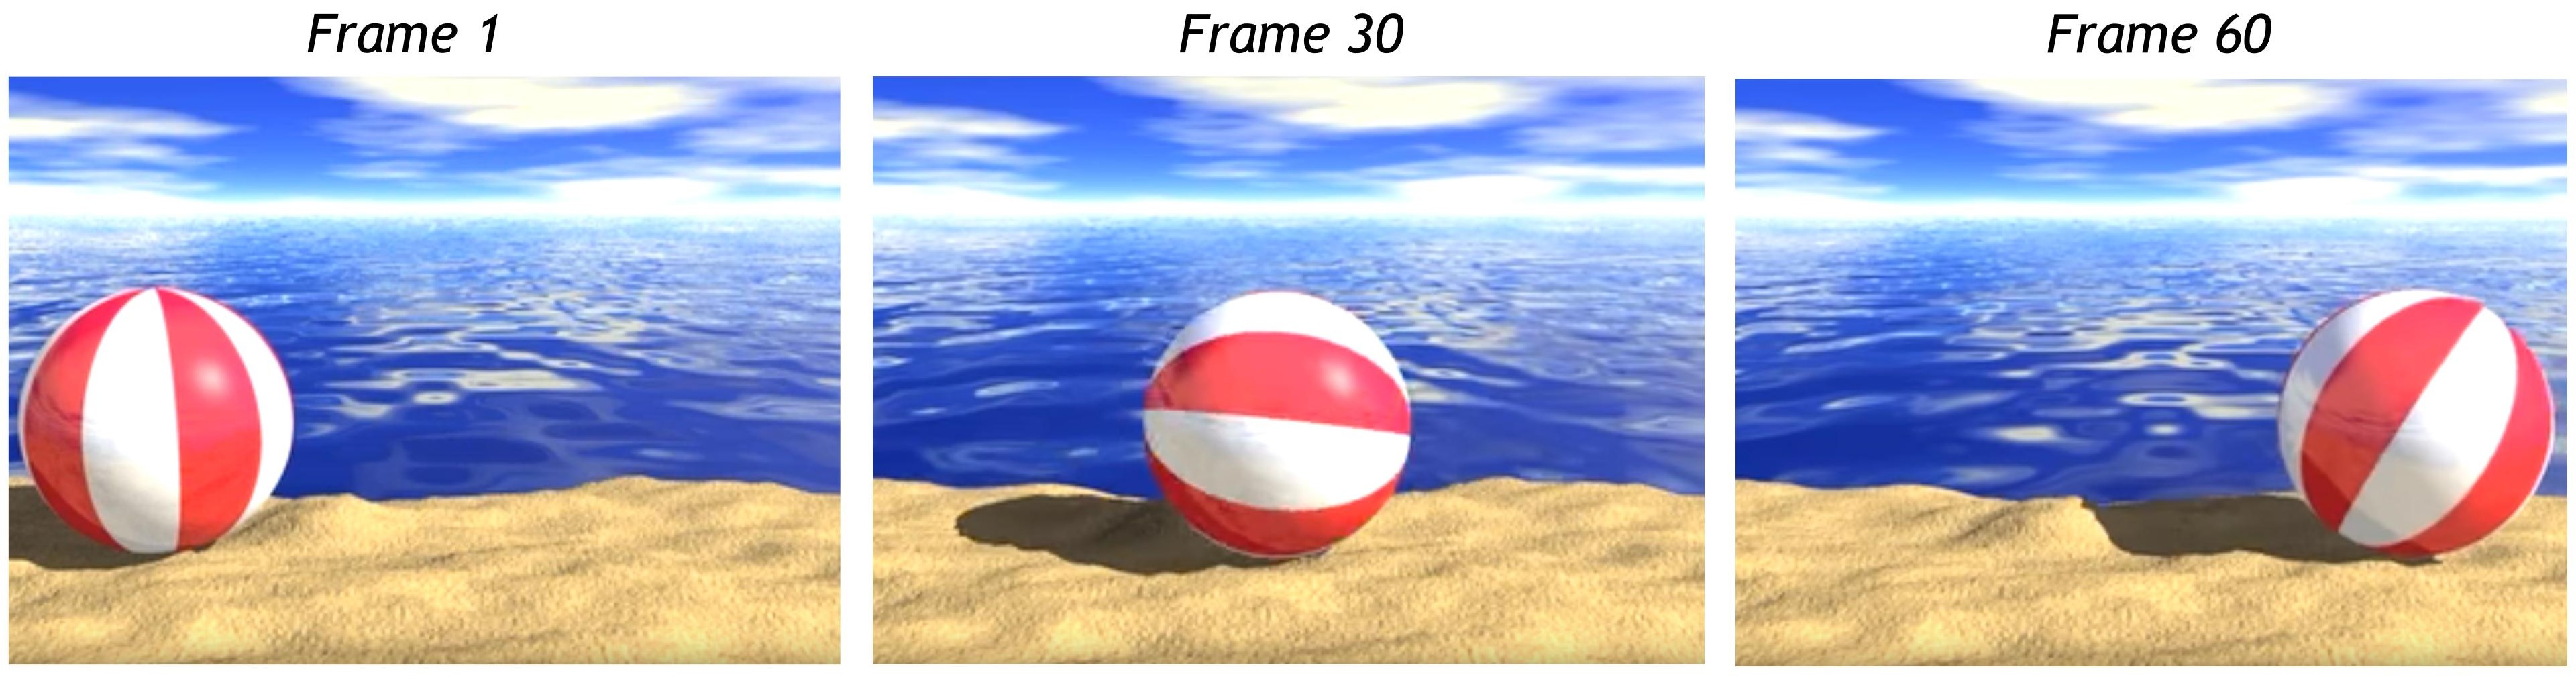
\includegraphics[width=\textwidth]{figures/ball_rolling.jpg}}
\caption{\label{fig:rolling_ball}Example of frames to sample for low-visual content analysis. The first frame for each second (one frame every thirty seconds) is retrieved for a 30 fps 3-second video of a ball rolling from the left-hand side of the screen to the right-hand side. Video frames courtesy of \textit{``How to Animate a Rolling Ball"} YouTube video available online: \url{https://youtu.be/cgbLAreElNI?t=130}.}
\end{figure}

\subsubsection{Thumbnails for Initial Shortlisting}

In their work, M. Okabe et al. \cite{okabe2018animating} generate thumbnails for each video in their database, which are stored as additional data along with the original video file. The thumbnails for the query video and for the database videos would be generated using the same algorithm in order to create similar results. This technique can be used in parallel to A. Araujo et al.'s \cite{araujo2017i2v}, who states that an initial shortlist of potentially matching videos can be generated before the main pattern matching phase. This shortlist can be created by computing the similarities between the query video's thumbnail and the thumbnails of the database videos.\\

Many advantages can be gained from this small initial step which could have an important impact on the system's overall speed and efficiency performance. Indeed, database videos that share no similarities to the query video will not be considered at all during the main pattern matching phase e.g. if the query video corresponds to a colourful sunset, then database videos of cloudy environments will be immediately filtered out as it is unlikely that they will match with the query video in the main pattern matching phase. This step diminishes the number of the videos to compare to the query.\\

This initial step is extremely speedy as it only uses a single frame that describes the entire video. Therefore the entire process will not be noticeably slowed down. However this concept could only be applied on relatively small databases where the videos contain a single scene with multiple similar shots. Indeed, shots can be characterised by a single still as they are made up of frames with similar visual content, whereas scenes can be made up of shots that change a lot and describe different visual content. Using thumbnails to shortlist a database of feature-length movies would greatly diminish the accuracy of the system due to the high number of scenes that make up a movie that cannot be resumed to a single thumbnail. The database videos' thumbnails will have already been generated during the database's pre-processing phase, which only occurs a single time. A possible solution could be to create a thumbnail for each shot in a scene, and store each thumbnail in a list. For example, if a scene contains six different shots, then six thumbnails will be generated to describe that scene.\\

\begin{comment}
\cite{okabe2018animating}
For quicker pattern matching and feature extraction, 16 pixels separate two feature points, allowing for rough pattern matching rather than exact pattern matching. This could be used when using feature-length movies as database videos to pattern match.
\end{comment}

% ----------------------------------------------------

\subsection{Fisher Vectors}

TODO:
\begin{itemize}
    \item Fisher Vectors can be used to generate a compact signature for videos, which will then be used for computing similarities between the query video's FV and the database videos' FVs \cite{araujo2017i2v}
\end{itemize}


%%%%%%%%%%%%%%%%%%%%%%%%%%%%%%%%%%%%%%%%%%%%%%%%%%%%%%%%%%%%%%%%%%%%%%%%%%%%%%%%%%
% 5 - CHAPTER SUMMARY
%%%%%%%%%%%%%%%%%%%%%%%%%%%%%%%%%%%%%%%%%%%%%%%%%%%%%%%%%%%%%%%%%%%%%%%%%%%%%%%%%%
\section{Chapter Summary}

chapter summary

% review the requirements decisions and critique the requirements process.
\chapter{Requirements}
\label{ch:chapter3}
This chapter establishes the requirements of the system. These requirements were devised in response to the problems mentioned in Section \ref{sec:problem-description} of Chapter \ref{ch:chapter1} and builds upon the information provided by the Literature and Technology Survey in Chapter \ref{ch:chapter2}.\\

The following requirements are divided between non-functional and functional sections, which are further split into more specific sections. They are prioritised using the words \textit{must} (Priority 1), \textit{should} (Priority 2) and \textit{may} (Priority 3); where \textit{must} indicates a crucial requirement to the system, \textit{should} an optimal requirement and \textit{may} a beneficial requirement.

\section{Functional Requirements}

\subsection{System Requirements}

To establish the system requirements, the system can be broken down into three phases. Based on the models described in the Literature \& Technology Survey in Section \ref{sec:color-based-features} and Section \ref{sec:litsurvey-models-pattern-matching}, and taking into consideration the time constraints and scope of the project, a training/testing approach is adopted. For each database video, features are extracted and stored in the first phase before being compared to a query's features in the second phase. A third phase can be added based on the video processing techniques stated in Section \ref{sec:movie-pre-processing}.

\subsubsection{Off-line Feature Extraction Phase}

These requirements concern the off-line feature extraction phase where the system learns by ingesting static unsupervised data corresponding to the database videos. In this phase, features are extracted from each video to generate feature vectors which are stored in files for the next phase.

\begin{enumerate}[label=F\arabic*]

    \item \textbf{The system \underline{must} run this phase a single time without requiring to be executed again for the next phase}.\\
    The features stored in files must be re-used in the next phase rather than being generated every time. The system \textbf{must} re-ingest the data whenever a change is carried out in the database e.g. a video has been added or a video has been removed.\\
    Priority 1.
    
    \item \textbf{Simple features that are proven to work efficiently with videos \underline{must} be chosen to be extracted.}\\
    Due to the nature of the project, a line must be drawn between the complexity of the feature being extracted to represent the videos and the efficiency of working with such a feature. For example, if the feature is very complicated to extract and use, but does not offer many more advantages than a simpler feature to extract and use, then the simpler feature should be used.\\
    Priority 1.
    
    \item \textbf{The system \underline{must} store the extracted features it used for learning in files for future re-use in the on-line retrieval phase.}\\
    Files can be saved either in plain text ``\textit{.txt}'' file format to be human-readable, or in other file formats such as binary ``\textit{.dat}'' files.\\
    Priority 1.
    
    \item \textbf{The files containing the training data \underline{must} be able to be quickly loaded into memory during the matching phase.}\\
    To minimise additional time spent on I/O operations, the files should be loaded quickly using efficient functions designed for this type of operation. If necessary, an external third-party library may be used to provided functions for quicker I/O operations.\\
    Priority 1.
    
    \item \textbf{The system's interface \underline{should} specify that it is ingesting and extracting features from the database videos.}\\
    It can do so by either displaying a loading spinner or by iteratively printing text specifying which video is being currently processed.\\
    Priority 2.
    
\end{enumerate}

\subsubsection{On-line Retrieval Phase}

These requirements concern the retrieval of the system, where the same extracted features from the previous phase are extracted from the query video and compared to the stored features from each database video by calculating the distance between between these features.

\begin{enumerate}[label=F\arabic*,resume]

    \item \textbf{The system \underline{must} accept a pre-recorded video as input.}\\
    This pre-recorded video will serve as the query video.\\
    Priority 1.
    
    \item \textbf{The system \underline{must} crop the recorded video to select a ``region of interest''.}\\
    The system must ignore the pixels outside of the selected area of the clip when extracting its features.\\
    Priority 1.
    
    \item \textbf{The system \underline{must} use well-known distance metrics to calculate the distances between the query's feature vectors and the database videos' feature vectors.}\\
    Hundreds of metrics exist, but some are more efficient for the task at hand. A good indication that a distance metric is good for the task at hand is its availability for popular programming languages and their mainstream third-party libraries.\\
    Priority 1.
    
    \item \textbf{The system \underline{must} display the results once the classification has been completed.}\\
    The retrieved video \textbf{must} be emphasised over the other videos to clearly point out that the result has been found. Additional results such as individual distances between the query and each video can be displayed as well e.g. tables.\\
    Priority 1.
    
    \item \textbf{The system \underline{must} be evaluated using reliable performance measurements.}\\
    The accuracy of the system should be calculated for different queries.
    Priority 1.
    
    \item \textbf{The system \underline{should} stabilise the query video before extracting its features.}\\
    The stabilised video will diminish the effects of camera movement and increase the similarities between the video's extracted features and the database videos' features.\\
    Priority 2.
    
    \item \textbf{The system \underline{may} be able to directly record a query video.}\\
    Processing the query video while it is being recorded would drastically improve the system's runtime in this phase rather than waiting for the entire video to be recorded and only processing it after the recording is finished.\\
    Priority 3.
    
    \item \textbf{The system \underline{may} find a match to the query in less than 10 seconds.}\\
    Commercial applications usually take around 10 seconds to produce a match to the query. Therefore, this project should take roughly the same amount of time before producing an output.\\
    Priority 3.
    
\end{enumerate}

\subsubsection{Database Pre-processing}

These requirements concern the database pre-processing phase of the system. This phase concerns the operations to carry out the the database videos to improve the off-line feature extraction and on-line retrieval phases.

\begin{enumerate}[label=F\arabic*,resume]

    \item \textbf{Long videos, e.g. feature-length movies, \underline{must} be processed for shot boundary detection to segment them into scenes.}\\
    A single frame must be used to represent each shot of a long video. However, this is not required if the video is short enough to be a shot by itself.\\
    Priority 1.
    
    \item \textbf{The same features from the off-line feature extraction and on-line retrieval phases \underline{should} be used for the shot boundary detection algorithm.}\\
    This would ensure cohesion between different phases of the program and allow code to be re-used.
    Priority 2.
    
\end{enumerate}

\subsubsection{General Requirements}

\begin{enumerate}[label=F\arabic*,resume]

    \item \textbf{The MVP\footnote{Minimum Viable Product} \underline{must} at least be a Command Line Interface that accepts command line inputs to run different phases of the program and enable/disable options.}\\
    A simple CLI is the minimum interface required to run the system with different arguments and to display results.\\
    Priority 1.
    
    \item \textbf{The system \underline{must} be able to run on a machine equipped with a terminal.}\\
    Any machine running Windows, Mac or Linux distributions should be able to run the system with the correct project dependencies installed.\\
    Priority 1.
        
    \item \textbf{The system \underline{should} include a ``README'' file with instructions on how to run the system.}\\
    The ``README'' file allows the system to be accessible to other users with the appropriate background knowledge to install the pre-required dependencies and run the system successfully.\\
    Priority 2.
    
    \item \textbf{The interface \underline{may} be a graphical interface.}\\
    For example, it could be a simple HTML web page or a native UI desktop application (which will depend on the chosen programming language). This would allow for information to be more clearly displayed on the screen.\\
    Priority 3.
        
\end{enumerate}

\subsection{Code Design Requirements}

\begin{enumerate}[label=F\arabic*,resume]

    \item \textbf{The system's code \underline{must} be source controlled using Git and backed up on GitHub in a private repository.}\\
    This will enable the code to be safely backed and offer a timeline of the system's development phase.\\
    Priority 1.
    	
	\item \textbf{The system \underline{should} follow coding style guidelines set for the programming language of choice.}\\
	This will ensure that the code will be written at the highest standard by following professional practices and will be more easily readable by industry experts.\\
	Priority 2.

	\item \textbf{The system \underline{should} use third-party libraries for complex aspects of the software to avoid rewriting complicated code that already exists and is easily accessible.}\\
	Rewriting code that already exists could be a waste of time for a project with such as shirt time-frame. Therefore, using third-party libraries will mean more time can be spent designing and implementing high-level concepts of the system.\\
	Priority 2.

    \item \textbf{The system \underline{may} be covered with unit tests and integration tests.}\\
    To ensure that different core aspects of the system work as expected, unit tests can be written around these sections. Additionally, multiple core aspects can be tested as a whole with integration tests.\\
    Priority 3.

\end{enumerate}

\subsection{Data Requirements}

\begin{enumerate}[label=F\arabic*,resume]

    \item \textbf{The videos used in the database \underline{must} not violate any copyright laws.}\\
    They must have licenses allowing them to be re-used for personal and commercial purposes at no cost.\\
    Priority 1.
    
    \item \textbf{The duration of the videos \underline{should} range from 7 to 14 seconds.}\\
    Working with short videos is enough to prove that the system pipeline works as intended since a considerable number of them can be used to populate the database, whereas only a handful of videos could be efficiently used if feature-length movies were used instead. 7 seconds is enough to ensure each video has at least 210 frames\footnote{Assuming videos with a frame rate of 30 fps.} to analyse.\\
    Priority 2.

    \item \textbf{There \underline{should} be a minimum of 50 unique videos in the database.}\\
    Because short videos rather than long ones are used to test the system pipeline, there should be a considerable amount of them to challenge the system.\\
    Priority 2.
    
    \item \textbf{The system pipeline \underline{may} be tested with a few feature-length movies as database videos.}\\
    The main goal of the project is to build the system pipeline, which can be tested with a database of many short videos rather than a database of a few long videos. To further explore the efficiency of the system, feature-length movies could be used to report the results when attempting to match them to a short query.\\
    Priority 3.
        
\end{enumerate}

\section{Non-Functional Requirements}

\begin{enumerate}[label=NF\arabic*]

    \item \textbf{The latest technologies \underline{must} be used to build the system.}\\
	The latest versions of programming languages and libraries must be used to ensure that the system takes advantage of up-to-date technology.\\
	Priority 1.
	
	\item \textbf{The system \underline{should} not be built with external users in mind.}\\
	It should only be run by the system's creator or users with a background in computer science who could understand how to run it using the README file provided.\\
	Priority 2.

    \item \textbf{The interface \underline{should} make the results easy to read.}\\
    This could be achieved with the use of large fonts, colours and bold text. Text used to discern the main results from less important output should be emphasized.
    
    \item \textbf{The system \underline{may} run smoothly and uninterrupted.}\\
    Priority 3.
    
    \item \textbf{The system \underline{may} not crash or exit unexpectedly with no error message.}\\
    Priority 3.

\end{enumerate}

\section{Summary}

This chapter has summarised the requirements needed to design and implement a successful system based on the problems formulated in Chapter \ref{ch:chapter1} Section \ref{sec:problem-description} and the Literature and Technology Survey from Chapter \ref{ch:chapter2}. Now that the requirements have been established, different potential solutions will be explored in the next chapter, including the benefits and disadvantages of each method, before one global solution can be chosen and implemented.

% review your design decisions at various levels and critique the design process.
\chapter{Design}
\label{ch:chapter4}
Now that the requirements necessary to build the system have been formulated, potential solutions to fulfil the list of requirements from Chapter \ref{ch:chapter3} for each aspect of the system can now be analysed before choosing a final solution. Throughout this chapter, the requirements established from the previous chapter referred as ``F'' stand for functional requirements, while requirements referred as ``NF'' stand for non-functional requirements. The first section of this chapter will focus on the programming language that will be used to build the system. Next, the second section explores different solutions for the system's pipeline, starting with the off-line feature extraction phase, followed by the on-line retrieval phase, and ending with the database pre-processing phase. Finally, the last section will focus on general design decisions such as the type of interface, the type of file to store the features in and the type of videos to populate the database with. These two sections are used to conclude the chapter with a detailed outline of the final chosen solutions for each aspect of the system, which are all used to eventually bring the system to life.

%%%%%%%%%%%%%%%%%%%%%%%%%%%%%%%%%%%%%%%%%%%%%%%%%%%%%%%%%%%%%%%%%%%%
%%%%%%%%%%%%%%%%%%%%%%%%%%%%%%%%%%%%%%%%%%%%%%%%%%%%%%%%%%%%%%%%%%%%
%%%%%%%%%%%%%%%%%%%%%%%%%%%%%%%%%%%%%%%%%%%%%%%%%%%%%%%%%%%%%%%%%%%%

\section{Programming Language}
\label{sec:design-programming-languages}

The programming language is one of the essential aspects when it comes to designing and later implementing the system as it is the medium used to transform the system from design to implementation. However, choosing between 250 different programming languages \cite{tiobe} can be a tricky exercise, which is why multiple views have to be evaluated before choosing a programming language. Various criteria are considered to justify the choice of the programming languages, including the availability of computer vision-related functions, the runtime speed, the readability and the personal preference.\\

The first element to consider when choosing a programming language for this type of project is the availability of functions for video manipulation and computer vision-related operations. Indeed, using high-level functions to, e.g. read videos or generate histograms is primordial to avoid spending time manually implementing each of these functionalities and to instead devote more time on implementing high-level concepts to complete the pipeline. Some languages such as MATLAB and Python (with mainstream third-party libraries) allow for efficient manipulation of images/videos and offer collections of computer vision functions. For other programming languages, libraries can be used. The most popular library in this field is OpenCV\footnote{OpenCV, \url{https://opencv.org/}}, which offers functions for real-time computer vision applications. This library supports all the main operating systems (Linux, macOS, Windows, etc.) and although it was mainly designed for C/C++, it contains bindings for the main general-purpose programming languages such as Python, C++, Java, C\#, Javascript, Haskell and MATLAB.\\

Among the previously mentioned programming languages, C/C++ are the fastest languages,
according to \textit{Benchmark Games}\footnote{Benchmark Games: \url{https://benchmarksgame-team.pages.debian.net/benchmarksgame/}}, followed by Java, MATLAB and Python, which is considerably slower than the aforementioned programming languages. However, Python can be extended with languages such as C/C++ with ease. This means that coupling Python with the OpenCV library that is initially written in C++ allows the Python code to execute as fast as the original C++ code since it is the actual OpenCV C++ code that is running in the background. Furthermore, Python has an extensive set of third-party libraries that add powerful functionalities to the language, such as NumPy\footnote{NumPy: \url{https://www.numpy.org/}}, SciPy\footnote{SciPy: \url{https://www.scipy.org/scipylib/index.html}} and Matplotlib\footnote{Matplotlib: \url{https://matplotlib.org/}}, which all add mathematical and scientific functions able to compete with MATLAB's native functions. Finally, of all the specified programming languages, Python is the favoured one in terms of personal preference, familiarity, and experience. Therefore, the relatively slower execution speeds of Python being outweighed when using OpenCV functions, coupled with the personal preference for Python, make Python the obvious programming language choice for this project.\\

For a complete review of the main pros and cons considered between when deciding between Python, C++, Java and MATLAB, refer to Appendix \ref{ch:appendix-comparison-programming-languages}.

%%%%%%%%%%%%%%%%%%%%%%%%%%%%%%%%%%%%%%%%%%%%%%%%%%%%%%%%%%%%%%%%%%%%
%%%%%%%%%%%%%%%%%%%%%%%%%%%%%%%%%%%%%%%%%%%%%%%%%%%%%%%%%%%%%%%%%%%%
%%%%%%%%%%%%%%%%%%%%%%%%%%%%%%%%%%%%%%%%%%%%%%%%%%%%%%%%%%%%%%%%%%%%

\section{Pipeline Design Analysis}

To chose a global design solution for the system, it is easier to break down the system's pipeline into different phases and review the numerous potential designs for each of these phases. Based on the models described in the Literature \& Technology Survey in Section \ref{sec:color-based-features} and Section \ref{sec:litsurvey-models-pattern-matching}, and taking into consideration the time constraints and scope of the project, histograms, which correspond to the simplest method listed, are used with a training/testing approach. Features are extracted and stored in histograms for database videos in the first phase before being compared to a query's histograms in the second phase. A third phase can be added for video processing techniques stated in Section \ref{sec:movie-pre-processing}. Therefore, the system pipeline can be split into three different phases, as shown in the concise diagram in Figure \ref{fig:basic-cbvr-diagram}:

\begin{itemize}
    \item \textbf{Off-line Feature Extraction Phase}. This phase corresponds to the ``training'' phase of the system, where features are extracted from each video in the database and then stored in data files to be later used in the on-line retrieval phase.
    \item \textbf{On-line Retrieval Phase}. This phase is affiliated to the ``testing'' phase of the system, where a single video query is matched to one of the database videos by extracting the same features from the previous phase and comparing them to the stored features.
    \item \textbf{Database Pre-processing Phase}. This is an optional phase where the database videos are processed before the off-line feature extraction phase to improve the accuracy and speed of the database videos feature extraction.
\end{itemize}

\begin{figure}[h]
\centerline{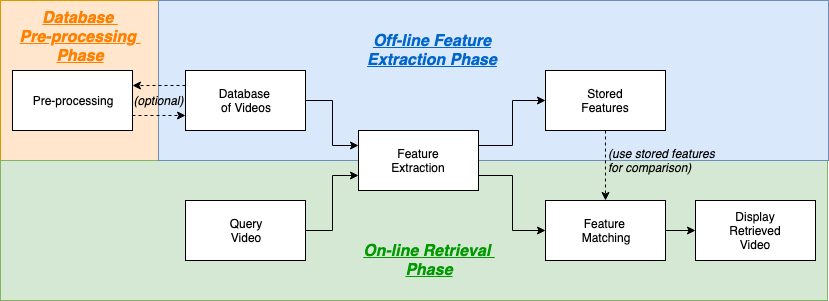
\includegraphics[width=1.1\textwidth]{figures/design/basic_cbvr_phases.png}}
\caption{\label{fig:basic-cbvr-diagram}Basic CBVR system diagram depicting a high-level pipeline separated into three phases.}
\end{figure}

\begin{comment}
Explore possible options for different sections of the system, such as:
    \begin{itemize}
        \item types of features to extract (why static colour features and not object/motion features) - histograms are very popular with videos, calculations are easier, implementation is easier, results are as efficient
        \item types of learning models (histogram matching, BoW-approach VS Neural Network)
    \end{itemize}
\end{comment}

%%%%%%%%%%%%%%%%%%%%%%%%%%%%%%%%%%%%%%%%%%%%%%%%%%%%%%%%%%%%%%%%%%%%

\subsection{Off-line Feature Extraction Phase}
\label{sec:design-offline-feature-extraction}

Retracing the Section \ref{sec:visual-content-extraction} of Literature \& Technology Survey, the first distinction between the possible types of features that could be extracted from the videos is static and dynamic features. Because static features extraction is a much less challenging task to code and to compute than dynamic feature extraction, while providing almost as much information as dynamic features and being cheaper to compute \cite{hu2011survey}, static features are therefore the logical choice for this project. However, there are many different choices of static features to extract, including colour-based, texture-based and shape-based features. Texture and shape-based features are more suitable for images than videos, while colour-based videos are suitable for both. Therefore, colour-based features are the features used to describe the videos, fulfilling requirement F2.\\

The most efficient type of model for representing colour-based features is histograms, which are described in Section \ref{sec:color-based-features}, Chapter \ref{ch:chapter2}. Different histograms exist for a variety of colour spaces depending on the application, with 2D histograms for \textit{greyscale} and \textit{RGB} colour spaces, and 3D histograms for the \textit{HSV} colour space. Because these are the three most used colour models for describing videos and their frames, and the most accessible ones based on the third-party libraries available for Python, they are the three histograms models chosen for colour feature extraction.\\ 

To maximise speed, a compact signature should be generated for each video. The inspiration of representing a video in a unique and compact signature originates from \cite{araujo2017i2v} who uses fisher vectors to construct compact signatures for the database videos and the query video. This project applies Araujo's idea of creating such a signature for the database videos and the query video to histograms, where histograms are generated for multiple frames of video and are then averaged into a single histogram for each model. Once generated, the feature vectors are then stored in files in order to be easily re-used in the on-line retrieval phase rather than being re-calculated in this phase every time. The design choices for storing the compact signatures, also known as ``feature vectors'', are explored in more detail in Section \ref{sec:design-feature-storing-file-type}. 

%%%%%%%%%%%%%%%%%%%%%%%%%%%%%%%%%%%%%%%%%%%%%%%%%%%%%%%%%%%%%%%%%%%%

\subsection{On-line Retrieval Phase}
\label{sec:design-online-retrieval}

\subsubsection{Similarity Measurement}
\label{sec:design-online-retrieval-similarity-measurement}

Histograms are discrete distributions of the extracted colour-based features. Therefore, the distance between two histograms can be used to establish how close they are to each other. As stated earlier in Chapter \ref{ch:chapter3}, a long list of metrics exists to calculate the distance between two discrete distributions. Therefore, the most common distance metrics can be used to perform the measurements. To determine which distance metrics to use, their availability in popular third-party libraries is analysed. With Python as the chosen programming language and the third-party libraries to use already decided, the metrics available can be explored from the OpenCV and SciPy libraries.\\

\textbf{OpenCV}, the Python computer vision library, offers multiple metrics to compare histograms, including the \textit{Correlation}, \textit{Chi-Square}, \textit{Intersection}, \textit{Hellinger Distance} using the Bhattacharyya coefficient, an \textit{alternative Chi-Square} and the \textit{Kullback-Leibler Divergence} \cite{opencv-histcomp}. All of the mentioned metrics can be used in the system, apart from the alternative Chi-Square distance and the KL Divergence. In the first hand, the alternative Chi-Square distance is more efficient when working with texture-based features rather than colour-based ones \cite{puzicha1997non}. In the second hand, the Kullback-Leibler Divergence is more aimed at calculating the loss of information between two different distributions rather than calculating the actual distance between them \cite{kurt2007kldivergence}. An additional advantage of using the OpenCV library to compare histograms, which is already mentioned in Section \ref{sec:design-programming-languages}, is the fact that the original C++ code is being executed to calculate the comparison itself, meaning that using OpenCV to compare histograms is the quickest option available, even quicker than writing custom distance functions directly in Python.\\

\textbf{SciPy}, the Python mathematics/science/engineering library, offers two more advanced statistical distance metrics to compare discrete distributions, including the Wassertein Distance\footnote{The Wassertein Distance is also referred to as the Earth Mover’s Distance.} and the Energy Distance, which are both perfectly suitable for comparing histograms.\\

Using these metrics from the OpenCV and SciPy libraries satisfies requirement F22 of using libraries to avoid re-writing code that would be less efficient than the libraries'. Based on the availability of distance metrics in OpenCV and SciPy, the following distance metrics will be used when implementing the system, fulfilling requirement F8:

\begin{itemize}
    \item OpenCV distance comparison metrics:
    \begin{itemize}
        \item Correlation
        \item Intersection
        \item Chi-Square (first version only)
        \item Hellinger (using the Bhattacharyya coefficient)
    \end{itemize}
    \item SciPy statistical distances:
    \begin{itemize}
        \item Wassertein Distance (Earth's Mover Distance)
        \item Energy Distance
    \end{itemize}
   
\end{itemize}

Smaller distance between two histograms using the aforementioned metrics translates to similarities between those histograms. Once the distance between the query video and each database video has been calculated, the smallest (or largest, depending on the metrics being used) distance is used to find the best match. The number of correct matches made, also known as \textit{true positives}, and the number of incorrect matches, also known as \textit{false positives}, can be used to evaluate the system's accuracy (see requirement F10).\\

Some metrics are more complex than others, which, coupled with the colour model used, means that some distances have more importance than others. Therefore, the importance of the distances depends on the colour space used, where grey scale histograms have a low importance as they only use one channel, RGB histograms have a medium importance as they use three channels, and HSV histograms have the highest importance as they describe the colours in a frame with more detail than RGB.

%%%%%%%%%%%%%%%%%%%%%%%%%%%%%%%

\subsubsection{Query Video Pre-processing}
\label{sec:design-query-video-processing}

Drastic improvements in accuracy can be found by pre-processing the query video. The query video corresponds to the video that a user records with a mobile-device and uses as input in the system in order to be matched with one of the database videos. A commercial application would allow the user to directly record a video from the application, which would, in turn, be used to extract its features and compare them to the features of the database videos. Based on current commercial computer vision systems, e.g. Shazam for music recognition, the system could even start processing the video as it is being written rather than waiting for it to be saved. However, these are design aspects that would be required if the system were to be released to the public on a large scale. This is not the case since the goal is to develop the matching algorithm and complete the pipeline, meaning the query video may be a recording of one of the database videos used as input once the program starts running in the on-line retrieval phase. To simulate a realistic query and a potential commercial system, the video should be pre-recorded through a mobile device and used , fulfilling requirement F6, rather than being recorded directly through a mobile application, as pointed out by the low-priority requirement F12.\\

Recording the query through a mobile device gives rise to multiple challenges, as specified in Section \ref{sec:litsurvey-cbvr-4-mobile-devices}. Indeed, some of those challenges include undesired camera movements due to shaking hands and the targeted screen itself not taking up the entire frame, resulting in queries of poor quality. The former can be fixed by applying video stabilisation to the video (requirement F11), while the latter can be solved by selecting a ROI\footnote{Region of Interest} (requirement F7). Nonetheless, selecting an ROI can be tricky as the query needs to be recorded in ideal conditions to maximise the matching accuracy. Four different types of query conditions are depicted in Figure \ref{fig:difference-query-video-issues}:
\begin{itemize}
    \item a) Ideal Query: allows for an accurate ROI selection.
    \item b) Down-scaled Query: requires more complex ROI selection as it is harder to detect the edges of the screen automatically. There is also a loss of information as an important section of the frame is excluded.
    \item c) Skewed Query: requires even more complex ROI selection and results in more loss of information.
    \item d) Incomplete Query: Greatly diminishes the system accuracy since part of the recorded video is missing.
\end{itemize}

\begin{figure}[h]
\centerline{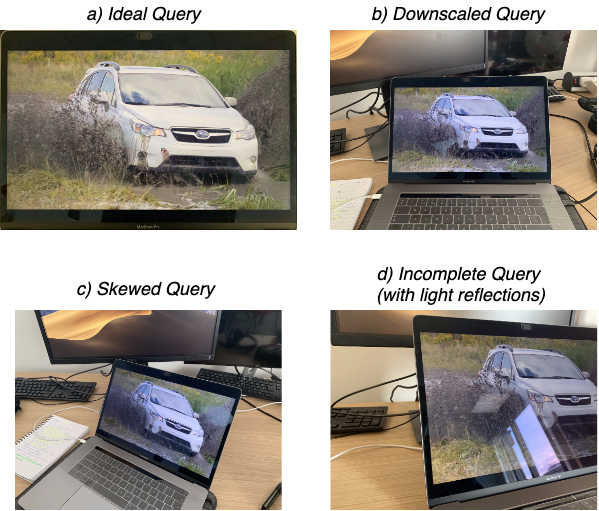
\includegraphics[width=0.8\textwidth]{figures/design/difference-query-video-issues.png}}
\caption{\label{fig:difference-query-video-issues}Different types of video queries, emphasising the contrast between what an idea query and poor quality queries would look like. All of these queries are often coupled with minor camera movement due to shaking hands.}
\end{figure}

On the grounds that the system should expect the worst case query, down-scaled and skewed queries should always be considered as the norm input. Ideal queries are rare as they depend on competent users with the knowledge of what defines a good video query. However, incomplete queries as shown in Figure \ref{fig:difference-query-video-issues}d should not be accounted for as it is near-impossible to match such a query to a database video accurately. Therefore, based on this analysis, the assumption that automatically selecting the ROI is a very complex task on its own can be made. Indeed, automatically detecting the edges of different screens to select the video being played as the ROI could grow to be even more intricate than the CBVR system itself. As a result, the ROI should be manually selected by choosing points on the query video to draw a contour around the screen. 

%%%%%%%%%%%%%%%%%%%%%%%%%%%%%%%%%%%%%%%%%%%%%%%%%%%%%%%%%%%%%%%%%%%%

\subsection{Database Pre-Processing Phase}

The database pre-processing phase's aim is to modify the database videos to improve the efficiency and speed of the feature vector generation. To achieve this, a shot boundary detection algorithm can be applied to each database video to extract a single frame per shot. This would cut down the size of a video to a tiny fraction of the original frames (ideally, one frame per shot), translating into fewer frames to be analyse when generating the average histogram. The global threshold approach, which is the simplest and most efficient one (see Section \ref{sec:litsurvey-shot-boundary-detection}, can be used to extract those frames. One of the distance metrics mentioned earlier in Section \ref{sec:design-online-retrieval-similarity-measurement} can be used to compare the histograms from consecutive frames, and detect shot boundaries when the distance is larger than the global threshold.

%%%%%%%%%%%%%%%%%%%%%%%%%%%%%%%%%%%%%%%%%%%%%%%%%%%%%%%%%%%%%%%%%%%%
%%%%%%%%%%%%%%%%%%%%%%%%%%%%%%%%%%%%%%%%%%%%%%%%%%%%%%%%%%%%%%%%%%%%
%%%%%%%%%%%%%%%%%%%%%%%%%%%%%%%%%%%%%%%%%%%%%%%%%%%%%%%%%%%%%%%%%%%%

\section{General Project Design}

Now that the design choices regarding the system pipeline have been made, general system choices such as the interface, the feature storage and the database videos can be inspected.

%%%%%%%%%%%%%%%%%%%%%%%%%%%%%%%%%%%%%%%%%%%%%%%%%%%%%%%%%%%%%%%%%%%%

\subsection{Interface}

With Python being the chosen programming language to implement the system and the type of query videos being decided, the next decision is the type of interface that is used to present the results. Although it was specified in Chapter \ref{ch:chapter1} that the system is meant to target mobile devices, creating a mobile application is a waste of time and resources for a project with such a narrow time frame. Although Python offers many choices of creating native GUIs using frameworks such as Tkinter, PyQt or WxPython, or merely creating HTML websites, building a graphical interface would take as much time as developing the entire system pipeline. Indeed, the primary goal is to complete the different phases of the pipeline that process and match a query video to a database video. Spending time on designing a GUI\footnote{Graphical User Interface} for a mobile device is unnecessary as the objective is not to create a commercial application that can be tested with users, as established in the requirements NF2, but to develop the matching algorithm that would work in the background of such an application.\\

The only pieces of information that need to be displayed are the following:
\begin{itemize}
    \item Progress of current phase, e.g. during the off-line feature extraction phase, specify how many videos have been processed and how many are left (see requirement F5). Visual cues, such as spinners, to can be used to indicate that work is being carried out by the program.
    \item Histograms: display the generated histograms for each video.
    \item Manual Cropping: display the video to have the user manually select the region of interest.
    \item Results (see requirement F9):
    \begin{itemize}
        \item The distance measurements between the query video and each database videos, while specifying which distance metric is used. Elegant output techniques such as tables could be used to display the results to satisfy requirement NF3.
        \item The final result, which should correspond to a thumbnail of the matched video.
        \item Additional data to measure the efficiency, e.g. the runtime and the accuracy (comparison of the number of true positives and the number of false positives)
    \end{itemize}
\end{itemize}

Most of the information previously mentioned can be displayed directly in the console, such as the current phase progress, the distance measurements and the efficiency results. The only graphical requirements are for the manual query cropping, the histograms and the final result output. The OpenCV GUI functions can be used to display the video in a new window and to manually draw the contour of the region of interest as automatically detecting the edges of the screen in the query video would be a very complicated task on its own. Regarding the histograms and the final result, it is crucial to show visual representations of the histograms and the matched video as it was noticed that during the demonstration of progress in February, only printing the title of the matched video did not provide a sense of accomplishment. Therefore, displaying the histograms and the matched video result can be done through Matplotlib, which is a library used to display plots (histograms) and images (thumbnail of the matched video). The combination of a CLI-based application supported by a few graphical interfaces meet requirement F16, while requirement F19 will only be fulfilled if time allows it as it is a low-priority requirement.

%%%%%%%%%%%%%%%%%%%%%%%%%%%%%%%%%%%%%%%%%%%%%%%%%%%%%%%%%%%%%%%%%%%%

\subsection{Feature Storing File Type}
\label{sec:design-feature-storing-file-type}

The features extracted during the off-line feature extraction phase (see Section \ref{sec:design-offline-feature-extraction}) and used during the on-line retrieval phase (see Section \ref{sec:design-online-retrieval}) can either be stored in text files or binary files. Due to the small amount of spread data (three histograms for each video) and the advantages of being able to view the data being written to the text files for debugging purposes, plain text files are the chosen file types for storing the features extracted from the database videos, satisfying requirement F3. Additionally, now that Python has been chosen as the programming language, functions from the NumPy library can be used to quick I/O operations when saving the data in plain text files, fulfilling requirement F4. For a complete review of the pros and cons between text files and binary files, see Appendix \ref{ch:appendix-comparison-text-vs-binary}.

%%%%%%%%%%%%%%%%%%%%%%%%%%%%%%%%%%%%%%%%%%%%%%%%%%%%%%%%%%%%%%%%%%%%

\subsection{Database videos}

Although the goal of the project is to eventually work with feature-length movies, the system will mainly be tested with short videos ranging between 7 and 14 seconds (see requirement F25). Indeed, using feature-length movies is not necessary to test the different stages of the system pipeline, and would not meet requirement F24 since they are copyrighted and not re-usable. A feature-length movie can be used to test the database pre-processing phase rather than the entire pipeline (see requirement F27), while the short videos can be used to test the combination of the off-line feature extraction and on-line retrieval phases.

%%%%%%%%%%%%%%%%%%%%%%%%%%%%%%%%%%%%%%%%%%%%%%%%%%%%%%%%%%%%%%%%%%%%
%%%%%%%%%%%%%%%%%%%%%%%%%%%%%%%%%%%%%%%%%%%%%%%%%%%%%%%%%%%%%%%%%%%%
%%%%%%%%%%%%%%%%%%%%%%%%%%%%%%%%%%%%%%%%%%%%%%%%%%%%%%%%%%%%%%%%%%%%

\section{Chosen Solution}

\begin{enumerate}
    \item \underline{\textbf{Programming Language}}: 
    \begin{enumerate}
        \item Python 3.7\footnote{Version 3.7 is the latest stable release of Python, satisfying NF1.}
        \item Third-party libraries:
        \begin{enumerate}
            \item OpenCV
            \item NumPy
            \item SciPy
            \item Matplotlib
        \end{enumerate}
    \end{enumerate}
    
    \item \underline{\textbf{Off-line Feature Extraction Phase}}:
    \begin{enumerate}
        \item \textbf{Types of feature}: static colour-based features in the form of colour histograms.
        \item \textbf{Types of Histograms Models}:
        \begin{enumerate}
            \item Greyscale
            \item RGB
            \item HSV
        \end{enumerate}
        \item \textbf{Feature Vector (Compact Signature)}: Averaged histogram (for each of the three histogram models)
    \end{enumerate}
    
    \item \underline{\textbf{On-line Retrieval}}: 
    \begin{enumerate}
        \item \textbf{Distance metrics}:
            \begin{enumerate}
                \item Correlation
                \item Intersection
                \item Chi-Square Distance
                \item Hellinger Distance
                \item Wassertein Distance
                \item Energy Distance
            \end{enumerate}
        \item \textbf{Query Video Pre-Processing}:
        \begin{enumerate}
            \item Video stabilisation
            \item ROI selection: manual
        \end{enumerate}
    \end{enumerate}
    
    \item \underline{\textbf{Database pre-processing}}: shot boundary detection algorithm using global threshold approach
    
    \item \underline{\textbf{Interface}}: Mainly command line for printing data, along with OpenCV GUI for the query video cropping and Matplotlib for displaying the histograms and results.
    
    \item \underline{\textbf{Feature Storing File Type}}: Plain Text (``.txt'') files.
    
    \item \underline{\textbf{Database Videos}}: Short license-free videos ranging between 7 and 14 seconds each.

\end{enumerate}

%%%%%%%%%%%%%%%%%%%%%%%%%%%%%%%%%%%%%%%%%%%%%%%%%%%%%%%%%%%%%%%%%%%%
%%%%%%%%%%%%%%%%%%%%%%%%%%%%%%%%%%%%%%%%%%%%%%%%%%%%%%%%%%%%%%%%%%%%
%%%%%%%%%%%%%%%%%%%%%%%%%%%%%%%%%%%%%%%%%%%%%%%%%%%%%%%%%%%%%%%%%%%%

\section{Summary}

With the main design aspects of the system pipeline phases laid out, along with an outline of the various system components such as the query video pre-processing operations, programming language, type of interface, type of storage feature file and type of videos used to populate the database, the system can finally be implemented in the next chapter.


% review the implementation and testing decisions and issues, and critique these processes.
\chapter{Implementation}
\label{ch:chapter5}
This chapter presents an overview of the different steps taken to fully implement a functional system by exploring the entire system pipeline. The chapter begins with the first stage of the pipeline, the off-line colour-based feature extraction phase, where histograms are extracted and averaged to create the feature vectors for each database video before being saved in files. Next, the second stage of the pipeline, the on-line retrieval phase, is covered, explaining how the query video is matched to one of the database videos using the compact histograms previously generated. Finally, the final optional stage of the pipeline is explored, the database pre-processing phase, explaining how videos can be segmented into denser videos. These three phases of the pipeline culminate with the flowchart diagram representing the entire system. Figures, mathematical formulas and code snippets are used to assist with examples and more precise visualisations. To round off the chapter, the approach used to gradually test the system during development is detailed, along with a coverage of the code structure of the project.

%%%%%%%%%%%%%%%%%%%%%%%%%%%%%%%%%%%%%%%%%%%%%%%%%%%%%%%%%%%%%%%%%%%%
%%%%%%%%%%%%%%%%%%%%%%%%%%%%%%%%%%%%%%%%%%%%%%%%%%%%%%%%%%%%%%%%%%%%
%%%%%%%%%%%%%%%%%%%%%%%%%%%%%%%%%%%%%%%%%%%%%%%%%%%%%%%%%%%%%%%%%%%%

\section{Off-line Colour-Based Feature Extraction}
\label{sec:implementation-offline-colour-based-feature-extraction}

This section details the different steps that go towards extracting colour features from the database videos to generate histograms and creating the feature vectors used to represent each video. The first step consists in establishing a selection of frames to process, followed by generating histograms for each of those selected frames. Once the histograms are generated, they are averaged into a single histogram before being normalised and stored into a plain text file.\\

Figure \ref{fig:implementation-rgb_average_histogram_pipeline} demonstrates a visual example of inner pipeline of this phase with RGB histograms only. This phase is repeated for greyscale and HSV histograms as well). The function controlling the execution process of this phase can be found in Appendix \ref{sec:code-off_line_colour_based_feature_extraction_phase}.\\

\begin{figure}[h] 
\centerline{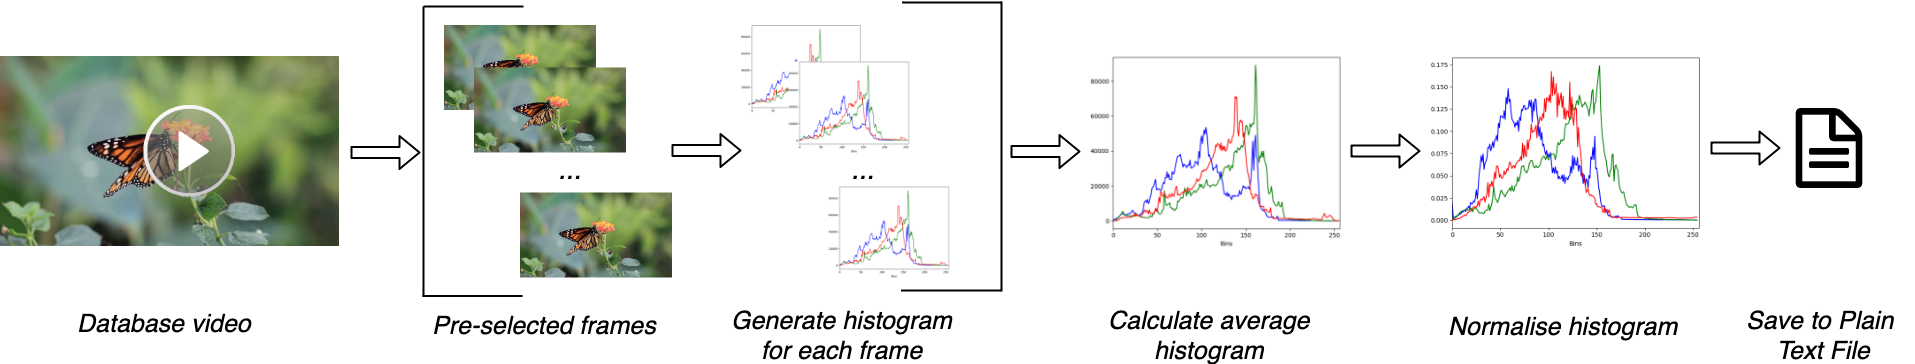
\includegraphics[width=1.2\textwidth,center]{figures/implementation/rgb_average_histogram_pipeline.png}}
\caption{\label{fig:implementation-rgb_average_histogram_pipeline}Visualisation of the pipeline of the off-line colour-based feature extraction phase with RGB histograms only.}
\end{figure}

This phase has to be repeated for every video in the database. For consistency throughout the various examples that are illustrated in this section, the \textit{butterfly} video is used to provide examples of the multiple off-line colour-based feature extraction steps.

%%%%%%%%%%%%%%%%%%%%%%%%%%%%%%%%%%%%%%%%%%%%%%%%%%%%%%%%%%%%%%%%%%%%

\subsection{Histogram Generation}

As described in Section \ref{sec:color-based-features}, a histogram represents the distribution of the pixels in a single frame. Different types of histograms can be generated based on the colour model used. This section covers how three types of histograms are constructed based on the colour model used, starting with greyscale histograms, followed by RGB histograms and ending with HSV histograms. Supporting code listings covering the generation of these three histograms can be found in the appendix, including the greyscale histograms in Appendix \ref{sec:code-single_grey_histogram_generation}, the RGB histograms in Appendix \ref{sec:code-single_rgb_histogram_generation}, the HSV histograms in Appendix \ref{sec:code-single_hsv_histogram_generation} and a high-level module overview of the \textit{HistogramGenerator} class and its functions in Appendix \ref{sec:code-high-level-module-overview}.

%%%%%%%%%%%%%%%%%%%%%%%%%%

\subsubsection{Greyscale Histogram}
\label{sec:implementation-greyscale-histogram}

The first type of histogram that is generated is the greyscale histogram, also known as an intensity-based histogram. This type of histogram is used with frames that are first converted to a black \& white colour space (see Figure \ref{fig:rgb_to_greyscale}), and thus has a single channel rather than the three traditional RGB channels found in colour images. The conversion is done using OpenCV's \textit{cv2.cvtColor()} function along with the \textit{cv2.COLOR\_BGR2GRAY} attribute: 

\begin{lstlisting}[numbers=none]
grey_frame = cv2.cvtColor(frame, cv2.COLOR_BGR2GRAY)
\end{lstlisting}

\begin{figure}[h] 
\centerline{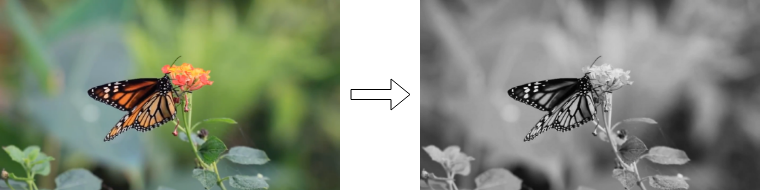
\includegraphics[width=\textwidth]{figures/implementation/rgb_to_greyscale.png}}
\caption{\label{fig:rgb_to_greyscale}Conversion of a frame from the RGB colour space to greyscale (black \& white).}
\end{figure}

Because the video frames are 8-bit images, the spectrum of the potential pixel values ranges between 256 possible values\footnote{$2^8=256$}. As a result, the histogram has 256 different bins from 0 to 255 to represent all the potential values that each pixel can take. The histogram itself is portrayed by Equation \ref{eq:grey-histogram}, where $g\in [0, 255]$ and $N_g$ represents the number of pixels that have an intensity equal to $g$. For example, $H(30)$ represents the number of pixels in the image with an intensity value of 30.
\begin{equation}
\label{eq:grey-histogram}
    H(g)=N_g
\end{equation}

The implementation of the greyscale histogram generation in the system is carried out through OpenCV's \textit{calcHist()} method, with the result portrayed in Figure \ref{fig:implementation-greyscale_not_normalised}. The grey frame is passed to the function, along with the number of channels to use, which is a single one in this case ($[0]$), an empty mask $None$ since the histogram is being calculated for the full frame, the number of bins $[256]$, and the range of values $[0, 256]$:

\begin{lstlisting}[numbers=none]
histogram = cv2.calcHist([grey_frame], [0], None, [256], [0,256])
\end{lstlisting}

\begin{figure}[h] 
\centerline{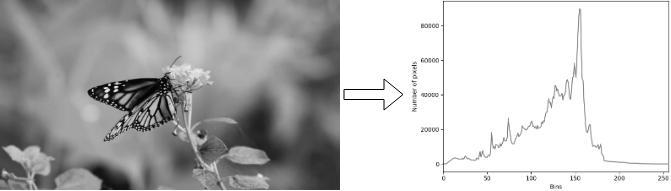
\includegraphics[width=\textwidth]{figures/implementation/greyscale_not_normalised.png}}
\caption{\label{fig:implementation-greyscale_not_normalised}The generated greyscale histogram (not normalised).}
\end{figure}

These greyscale histograms are generated for multiple frames of the video, but not all the frames as this would be highly inefficient, as explained in Section \ref{sec:litsurvey-challenges-temporality}. Indeed, rather than generating a histogram for each frame, which would be extremely inefficient and waste of computations, a selection of frames can be made in advance, which is then used for the histogram generation. Ideally, the frames extracted from the shot boundary detection algorithm later described in Section \ref{sec:database-pre-processing} would be used. However, because the range of the duration of the videos used is between 7 and 14 seconds and they are only made of a single shot, the shot boundary detection algorithm would only extract one frame from the videos. Therefore, for the purpose of building a realistic system, one frame is extracted every second to build up the selection of frames, using the \textit{\_get\_frames\_to\_process()} function, which can be found in Appendix \ref{sec:code-get_frames_to_process}. For example, with the butterfly video that contains 301 frames and has a frame rate of 30 frames per second, 11 frames are selected to generate a greyscale histogram (frames \textit{[1, 31, 61, ..., 271, 301]}).\\

Once the greyscale histograms are generated for each of these pre-selected frames, they are all stored away in a list, ready to be later averaged into a single histogram that will be used as the first feature vector to represent the entire video (see Section \ref{sec:implementation-compact-video-signature}).

%%%%%%%%%%%%%%%%%%%%%%%%%%

\subsubsection{RGB Histogram}

Now that greyscale histograms are generated for the video, RGB histograms are produced next. As described in \ref{sec:color-based-features}, an RGB histogram represents the colour distribution of the pixels in a frame for three different channels: red, blue and green. The coloured frame is a combination of three colour channels, which can be split into three different stills, as rendered in Figure \ref{fig:implementation-rgb_image_channel_split}.

\begin{figure}[h] 
\centerline{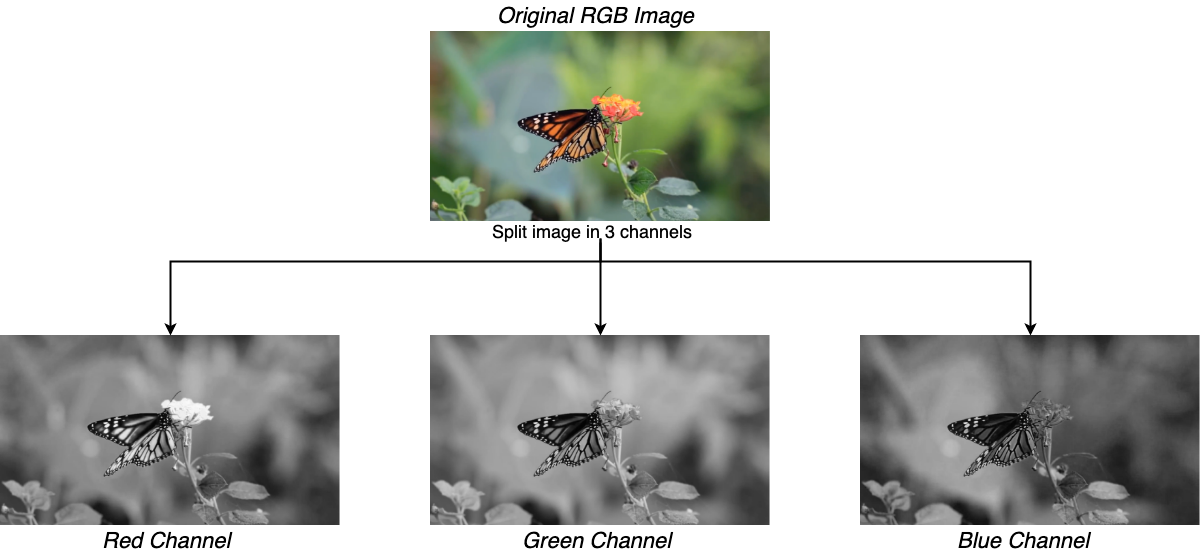
\includegraphics[width=\textwidth]{figures/implementation/rgb_image_channel_split.png}}
\caption{\label{fig:implementation-rgb_image_channel_split}The three colour channels that make up an coloured RGB image.}
\end{figure}

The RGB histogram is similar to the previously mentioned greyscale histograms, except that there are three separate histograms rather than a single one. There is, therefore, a 2D histogram for each colour channel (one in red, one in blue and one in green), where the brightness levels of each pixel are represented for each of those three colour channels. Each of the stills resulting from the split depicted in Figure \ref{fig:implementation-rgb_image_channel_split} will have their own histograms, which will form a complete RGB histogram when merged.\\

In contrast to the greyscale histograms, frames do not need to be converted to a different colour space when constructing RGB histograms as they are directly imported into three channels by OpenCV's \textit{cv2.VideoCapture()} function. In a similar fashion to the greyscale histograms, 256 bins are used for the RGB histograms, representing the potential values that each pixel can take for each colour channel. The RGB histogram is a combination of three 2D histograms, which are illustrated by Equation \ref{eq:rgb-histogram}, where $g_i\in [0, 255]$ and $N_g(i)$ represents the number of pixels that have an intensity equal to $g$ for the colour channel $i$. For example, $H_{i=2}(60)$ represents the number of pixels in the third channel of the image (blue channel) with an intensity value of 60.

\begin{equation}
\label{eq:rgb-histogram}
    \sum_{i=0}^{2} H_i(g)=N_g[i]
\end{equation}

To implement RGB histograms in the system, OpenCV's \textit{calcHist()} is once again used. In an identical manner to the greyscale histogram, the frame is passed to the function along with the colour channel \textit{[i]}, which are all placed inside a for-loop to generate a histogram for the three colour channels:

\begin{lstlisting}[numbers=none]
histogram = cv2.calcHist([frame], [i], None, [256], [0, 256])
\end{lstlisting}

At this point, the three individual histograms that have been generated for the three colour channels are merged into a single plot to build the RGB histogram, as depicted in Figure \ref{fig:implementation-rgb_not_normalised}.

\begin{figure}[h] 
\centerline{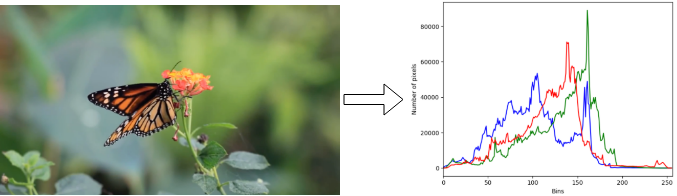
\includegraphics[width=\textwidth]{figures/implementation/rgb_not_normalised.png}}
\caption{\label{fig:implementation-rgb_not_normalised}The combination of the generated histograms for the three colour channels to construct the RGB histogram (not normalised).}
\end{figure}

Now that RGB histograms have been generated for each of the pre-selected frames (one frame every second), they are all stored in a dictionary made up of three keys, one for each colour channel. Each key links to a list where the histograms are stored away before being averaged into a single histogram used to create the second feature vector. 

%%%%%%%%%%%%%%%%%%%%%%%%%%

\subsubsection{HSV Histogram Generation}

With the greyscale and RGB histograms now formed, the HSV histograms can finally be generated. HSV histograms make use of the HSV colour space, requiring the video frames to be converted from the original RGB colour space to the HSV colour space (see Figure \ref{fig:rgb_to_hsv}). The conversion is done using OpenCV's \textit{cv2.cvtColor()} function along with the \textit{cv2.COLOR\_BGR2HSV} attribute:

\begin{lstlisting}[numbers=none]
hsv_frame = cv2.cvtColor(frame, cv2.COLOR_BGR2HSV)
\end{lstlisting}

\begin{figure}[h] 
\centerline{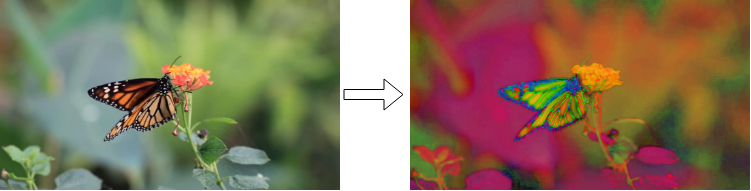
\includegraphics[width=\textwidth]{figures/implementation/rgb_to_hsv.png}}
\caption{\label{fig:rgb_to_hsv}Conversion of a frame from the RGB colour space to the HSV colour space.}
\end{figure}

This type of histogram is more complex to generate as it is not a 2D histogram like the previous greyscale and RGB histograms, but a 3D histogram. Because they are represented in 3D rather than 2D due to the particularities of the HSV colour space, less bins can be used to plot the data as pixels fall into bins when they are in conjunction with the range of the three channels (the pixels values must be within the range of the hue \underline{AND} the saturation \underline{AND} the value). Therefore, to avoid creating a histogram that is neither too coarse nor too sparse, 8 bins are used for the hue channel, 12 bins are used for the saturation channel, and 3 bins are used for the value channel, resulting in a histogram of 288 values\footnote{$8*12*3=288$}. This histogram is approximately the same length as the $256$ values previously used for the greyscale histograms and $3*256$ values for the RGB histograms. The histogram is described by Equation \ref{eq:hsv-histogram}, where $N(h,s,v)$ represents the number of pixels that fall within the range of the bin with values $h$ \underline{AND} $s$ \underline{AND} $v$.\\
\begin{equation}
\label{eq:hsv-histogram}
    H(h,s,v)=N(h,s,v)
\end{equation}

For example, a pixel with values $H(h=31, s=245, v=200)$ will fall into a bin with\footnote{Assuming ranges of 0-180 for Hue, 0-256 for Saturation, 0-256 for Value.}:
\begin{itemize}
    \item a hue value between 22.5 and 45 (bin \#2/8) \underline{AND}
    \item a saturation value between 234.6 and 256 (bin \#12/12) \underline{AND} 
    \item a value intensity between 170.7 and 256 (bin \#3/3).
\end{itemize}
The number of pixels in this bin will be $N(1,11,2)$ (0-based indexes).\\

Implementing the calculation of an HSV histogram in the system is again achieved through the use of OpenCV's \textit{calcHist()} function, with the result shown in Figure \ref{fig:implementation-hsv_not_normalised}. Similar arguments are passed such as the frame and an empty mask, but the arguments controlling the size of the histogram are different. In the code snippet below, \textit{[0, 1, 2]} indicates that the histogram has three channels (H, S and V), \textit{(8, 12, 3)} specifies the number of bins for each channel, and \textit{[0, 180, 0, 256, 0, 256]} marks the ranges of these bins:

\begin{lstlisting}[numbers=none]
histogram = cv2.calcHist([hsv_frame], [0, 1, 2], None, (8, 12, 3), [0, 180, 0, 256, 0, 256])
\end{lstlisting}

\begin{figure}[h] 
\centerline{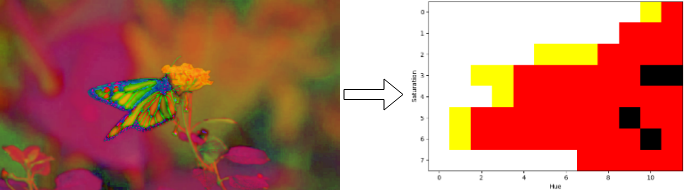
\includegraphics[width=\textwidth]{figures/implementation/hsv_not_normalised.png}}
\caption{\label{fig:implementation-hsv_not_normalised}The generated 3D HSV histogram (not normalised).}
\end{figure}

To conclude this first step of the off-line colour-based extraction phase, HSV histograms are finally generated. Once all the HSV histograms are generated for each pre-selected frame, they are all stored in a list, like for the greyscale and RGB histograms. With the greyscale, RGB and HSV histograms now all generated for each pre-selected frame of the video; these can now be averaged to create one feature vector for each histogram, which is explained in the next section.

%%%%%%%%%%%%%%%%%%%%%%%%%%%%%%%%%%%%%%%%%%%%%%%%%%%%%%%%%%%%%%%%%%%%

\subsection{Video Feature Vector Generation}
\label{sec:implementation-compact-video-signature}

At this stage of the off-line colour-based extraction phase, multiple greyscale, RGB and HSV histograms have been generated for each pre-selected frame for a video. Each of these histograms can now be averaged into one single histogram per colour model for each video. This means that each database video will be represented by one averaged greyscale histogram, one averaged RGB histogram and one averaged HSV histogram, which will constitute the feature vectors of the video. This is achieved by looping through all the histograms' bins generated per video and calculating a new averaged value for each bin. For reminders, this process is repeated for every video in the database. Supporting code listings covering the generation of the feature vectors for the three histogram models can be found in the appendix, including the greyscale histograms in Appendix \ref{sec:code-generate_and_store_average_grey_histogram}, the RGB histograms in Appendix \ref{sec:code-generate_and_store_average_rgb_histogram} and the HSV histograms in Appendix \ref{sec:code-generate_and_store_average_hsv_histogram}.\\

For the \textbf{greyscale histograms}, the 256 bins of the $N$ generated histograms are looped through and averaged (see Equation \ref{eq:average-greyscale-histogram}) to create a new mean value, where $H_n(i)$ corresponds to the number of pixels for the video's $n^{th}$ histogram at pixel intensity $i$.
\begin{equation}
\label{eq:average-greyscale-histogram}
    \sum_{n=0}^{N} \frac{\sum_{i=0}^{255} H_n(i)}{N}
\end{equation}

The averaged value is then stored into the corresponding $i_{th}$ bin of the new histogram. For example, if $N=10$ (the video had ten pre-selected frames, so ten greyscale histograms were generated for that video), then for each of the 256 bins, the values of the ten histograms at that bin are averaged and the mean is stored in the new histogram.

\begin{figure}[h] 
\centerline{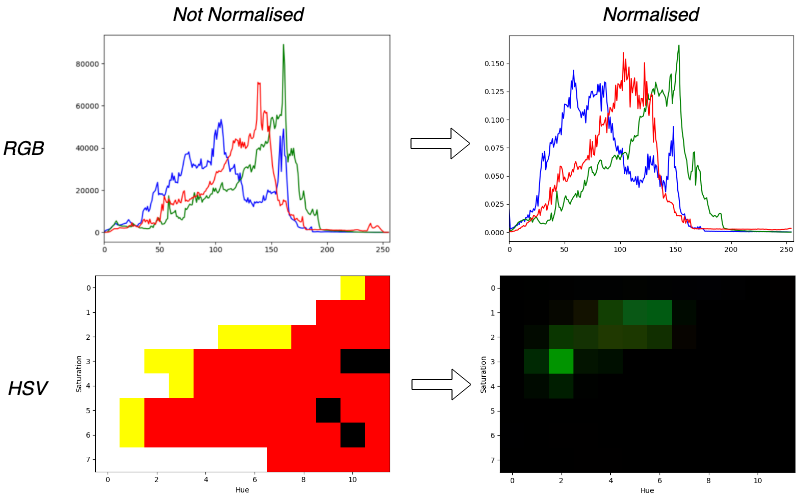
\includegraphics[width=\textwidth]{figures/implementation/normalise-histogram.png}}
\caption{\label{fig:implementation-normalise-histogram}Normalising RGB and HSV histograms.}
\end{figure}

Once all the bins have been averaged and added to the new histogram, that averaged histogram is normalised to obtain scale invariance between the histograms of the different videos. Instead of representing the number of pixels that fall into a bin, a normalised histogram represents a relative percentage count of the number of pixels in each bin, as depicted in Figure \ref{fig:implementation-normalise-histogram}. This is a necessary step in cases where the video frames have different sizes (the larger frames to have more pixels than the smaller frames) as the histograms can be more accurately compared when they represent a relative percentage rather than an integer count. The normalisation is achieved through OpenCV's \textit{cv2.normalize()} function:

\begin{lstlisting}[numbers=none]
histogram = cv2.normalize(histogram, histogram)
\end{lstlisting}

Finally, the averaged and normalised histogram values are stored in a plain text file as float values to maintain the precision, which is implemented using NumPy's \textit{np.savetxt()} function:

\begin{lstlisting}[numbers=none]
np.savetxt("../histogram_data/{}/hist-{}".format(self.file_name, "gray"), avg_histogram, fmt='%f'))
\end{lstlisting}

With the first feature vector in the form of an averaged and normalised greyscale histogram now stored in a plain text file, the same steps are repeated for the RGB and HSV histogram, with a few differences in the loops. First, for the \textbf{RGB histograms}, identical steps to the greyscale histogram's are followed for the three colour channels rather than a single time (see Equation \ref{eq:average-rgb-histogram}).

\begin{equation}
\label{eq:average-rgb-histogram}
    \sum_{h}^{(r,g,b)} (\sum_{n=0}^{N} \frac{\sum_{i=0}^{255} H_{h,n}(i)}{N_h})
\end{equation}

Second, for the \textbf{HSV histograms}, the histogram averaging is done by looping through each hue, saturation and value bin, since it is a 3D histogram and not a 2D histogram (see Equation \ref{eq:average-hsv-histogram}).

\begin{equation}
\label{eq:average-hsv-histogram}
    \sum_{n=0}^{N}(\sum_h \sum_s \sum_v H_n(h,s,v))
\end{equation}

Finally, the \textit{cv2.normalize()} and \textit{np.savetxt()} functions are used to normalise and save the average RGB and HSV histograms to plain text files. Examples of the saved plain text files for the butterfly video can be found in Appendix \ref{sec:appendix-txt-greyscale} for the greyscale histogram, in Appendix \ref{sec:appendix-txt-rgb} for the RGB histogram and in Appendix \ref{sec:appendix-txt-hsv} for the HSV histogram.\\

The final result of the off-line colour-based feature extraction phase is a set of three averaged histograms that represent an entire video, with the values saved in three separate plain text files, as depicted in Figure \ref{fig:implementation-all_avg_norm_histograms}.\\

Thanks to an argument parsing function written at the start of the program (see Appendix \ref{sec:code-listings-argument-parsing}), there is a choice to display these histograms using Matplotlib while they are being generated based on a flag passed on program startup. If the \textit{``showhists''} flag is passed, then all averaged histograms are displayed before being saved in plain text files.\\

As it takes approximately three seconds to process a single video in order to generate and store the three averaged histograms, the entire phase can take a while depending on the number of videos in the database. Therefore, a spinner is employed to indicate that the system is performing computations, which is implemented using Py-Spin\footnote{Py-Spin: \url{https://github.com/lord63/py-spin}}, a third-party library used to implement console-based spinners. The spinner, coupled with the histograms being displayed as they are being calculated, gives a visual indication that progress is being made.\\

With the colour-based features now saved in text files, they can be used multiple times in the on-line retrieval phase without needing to be regenerated, unless changes are made to the database videos, e.g. adding or removing videos.

\begin{figure}[h] 
\centerline{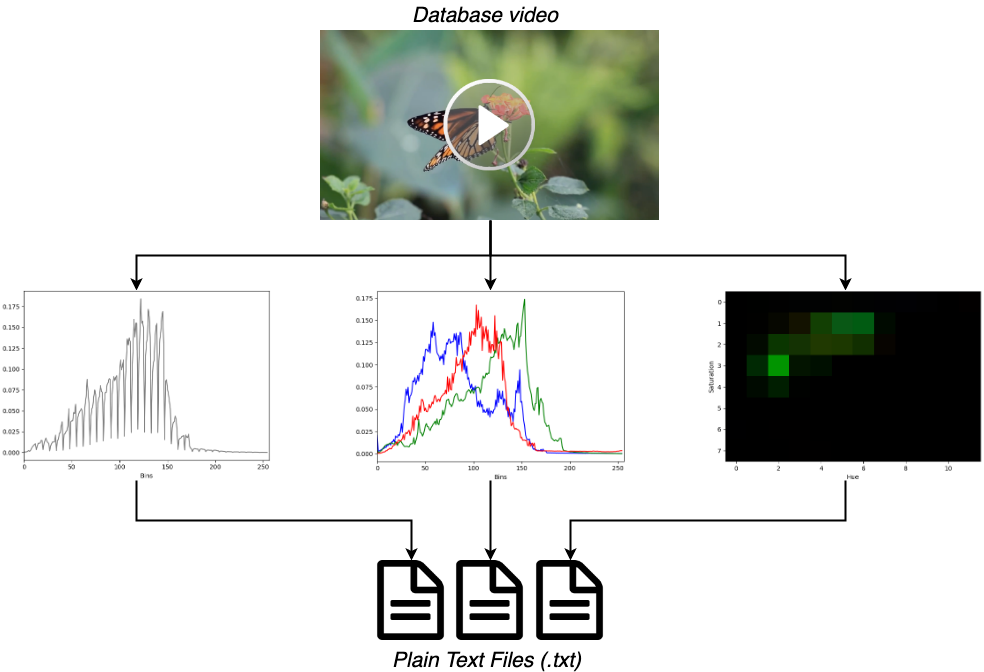
\includegraphics[width=\textwidth]{figures/implementation/all_avg_norm_histograms.png}}
\caption{\label{fig:implementation-all_avg_norm_histograms}The three average histograms generated for each database video and saved in plain text files.}
\end{figure}

%%%%%%%%%%%%%%%%%%%%%%%%%%%%%%%%%%%%%%%%%%%%%%%%%%%%%%%%%%%%%%%%%%%%
%%%%%%%%%%%%%%%%%%%%%%%%%%%%%%%%%%%%%%%%%%%%%%%%%%%%%%%%%%%%%%%%%%%%
%%%%%%%%%%%%%%%%%%%%%%%%%%%%%%%%%%%%%%%%%%%%%%%%%%%%%%%%%%%%%%%%%%%%

\clearpage
\section{On-line Retrieval}

This section details the different steps that go towards matching a query video to one of the database videos using the colour-based features extracted in Section \ref{sec:implementation-offline-colour-based-feature-extraction}. The first step consists in processing the recorded query video to get rid of undesired artefacts such as poor framing (e.g. camera not properly positioned) and unwanted camera movements (e.g. shaky camera). Once the query is finished being processed, the same colour-based features previously extracted for all the database videos in the form of greyscale, RGB and HSV histograms are used to compute the similarities between the query video and each database video by measuring the distance between the histograms. The video with the highest score will be the match found by the system, which is displayed to the screen to show the final result. The initial function controlling the execution process of this phase can be found in Appendix \ref{sec:code-on_line_retrieval_phase}.

%%%%%%%%%%%%%%%%%%%%%%%%%%%%%%%%%%%%%%%%%%%%%%%%%%%%%%%%%%%%%%%%%%%%

\subsection{Query Video Pre-processing}

\subsubsection{Video Stabilisation}

The first improvement that can be made to the query is video stabilisation. Video stabilisation is implemented through the VidStab\footnote{Python Video Stabilisation: \url{https://github.com/AdamSpannbauer/python_video_stab}} third-party library, which is a quick solution to prune query videos with shaky movements. Additionally, an option to extend the query's borders to maintain the original frame size is available to prevent losing information. The library is implemented in a custom class, which can be found in Appendix \ref{sec:code-VideoStabiliser}.\\

A ``yes/no'' question is displayed on the console, giving a choice to stabilise the query video or not. If ``yes'' is chosen, the system first checks if a potential version of the video has already been previously stabilised and stabilises the query if it has not been stabilised already. Similarly to the previous phase, a spinner is used to indicate that the video is being stabilised as the process takes around twenty seconds for a ten second-long video. If ``no'' is chosen, then the system again checks for potential stabilised versions to use; otherwise, it uses the original version.

\subsubsection{Region of Interest Selection}

The second improvement that can be carried out to the query is selecting a Region Of Interest (ROI). Selecting an ROI involves cropping the query video to select only the area with the actual object of interest. In this case, this involves selecting the video playing on a display.\\

ROI selection is achieved through OpenCV's GUI functionality, which is employed through multiple functions such as a function to display images using \textit{cv2.imshow()}, one to draw on the displayed images using \textit{cv2.rectangle()}, and one to record mouse events by writing a callback function named \textit{click\_and\_crop()}:

\begin{lstlisting}[numbers=none]
cv2.setMouseCallback("Select ROI", self.click_and_crop)
\end{lstlisting}

These three functionalities are combined in the system to display the first frame of the query video and allow a manual selection of two points on the frame. The first point is selected when the left mouse button is pressed using \textit{cv2.EVENT\_LBUTTONDOWN}, and the second point is selected when the button is unpressed using \textit{cv2.EVENT\_LBUTTONUP}. With these two points, a rectangle can be drawn on the frame to indicate the area that was selected. If the rectangle is correctly drawn, the \textit{`C'} key can be pressed to perform the cropping action; otherwise the \textit{`R'} key can be pressed to erase the rectangle and attempt to re-draw it until a satisfactory ROI is selected. The point coordinates are then used to ignore all the pixels outside the drawn rectangle when generating the query video's histograms, as sketched in Figure \ref{fig:implementation-roi_selection}. The full implementation of the ROI selection class can be found in Appendix \ref{sec:code-ClickAndDrop}.\\

\begin{figure}[h] 
\centerline{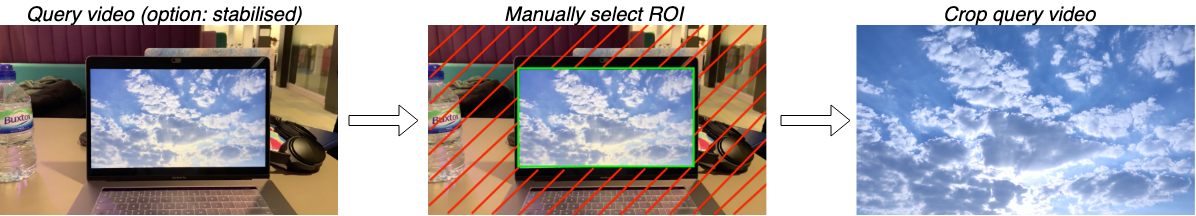
\includegraphics[width=\textwidth]{figures/implementation/roi_selection.png}}
\caption{\label{fig:implementation-roi_selection}The process of manually selecting a ROI to crop the query video.}
\end{figure}

Once the video query has been processed for stability and ROI selection, the same feature vectors from the off-line extraction phase can be generated before being compared to the database videos' feature vectors.

%%%%%%%%%%%%%%%%%%%%%%%%%%%%%%%%%%%%%%%%%%%%%%%%%%%%%%%%%%%%%%%%%%%%

\subsection{Matching Query to a Database Video}

\subsubsection{Query Video Feature Extraction}

In order to compare the query video to all the database videos, the same colour-based features described in Section \ref{sec:implementation-offline-colour-based-feature-extraction} need first to be extracted and the feature vectors calculated. Three feature vectors are generated for the query video in the form of an averaged greyscale histogram, an averaged RGB histogram and an averaged HSV histogram. To avoid code duplication, the same functions written for the off-line colour-based feature extraction phase are re-used to generate the query video's histograms. This is achieved through a function parameter named \textit{is\_query}, which is a boolean that enters more sections of the function when it is true, such as selecting an ROI:

\begin{lstlisting}[numbers=none]
def generate_video_rgb_histogram(self, is_query=False, cur_ref_points=None):
\end{lstlisting}

Once these histograms are generated, they can be compared to the histograms of each database videos.

\subsubsection{Distance Measurements}
\label{sec:implementation-distance-measurements}

At this stage of the pipeline, all of the feature vectors for the database videos and the query video have now been created and can be used to compute the similarities between them. The similarity measurements are done by calculating the distance between each of the database videos' histograms with the query video's histograms. Four different distance metrics are used to compare the 2D greyscale and RGB histograms, while two distance metrics are used to calculate the similarities between the 3D HSV histograms. Supporting code listings covering the distance calculation between 2D and 3D histograms can be found in Appendix \ref{sec:code-histogram-matching-2d-and-3d}.\\

The calculations between two 2D histograms are achieved through OpenCV's \textit{cv2.compareHist()} function, where the two histograms to compare are passed along with the method of choice:

\begin{lstlisting}[numbers=none]
comparison = cv2.compareHist(query_hist, rgb_video_hist, method)
\end{lstlisting}

For the 3D HSV histograms, SciPy's statistical distances are used to calculate the distance between the different bins. Different functions are used between the 2D and 3D histograms as OpenCV's \textit{cv2.compareHist()} function does not work with 3D arrays, whereas SciPy's statistical distances does. The six different methods used are detailed below, where $d(H_1, H_2)$ represents the distance between a histogram $H_1$ and a histogram $H_2$, and $I$ represents the number of bins in the histograms.\\

\begin{enumerate}

    \item \underline{Correlation}:\\
    This is a metric that indicates the linear relationship between two histograms. The result of this metric ranges between $-1 < d(H_1,H_2) < 1$, where -1 represents a negative correlation, 0 an absence of correlation and 1 a high positive correlation. The closer the two histograms are to each other, the closer their correlation will be to 1. Equation \ref{eq:correlation} describes how this metric can be calculated.
    \begin{equation}
    \label{eq:correlation}
        d(H_1,H_2)=\frac{\sum _I(H_1(I)-\bar{H_1})(H_2(I)-\bar{H_2})}{\sqrt{\sum _I(H_1(I)-\bar{H_1})^2(H_2(I)-\bar{H_2})^2}}
    \end{equation}
    where $\bar{H_k}=\frac{1}{N}\sum_JH_k(J)$ and $N$ is equal to the total number of bins in the histogram. This metric is available through OpenCV's \textit{cv2.HISTCMP\_CORREL} attribute:
\begin{lstlisting}[numbers=none]
comparison = cv2.compareHist(query_hist['grey'], dbvideo_hist_grey, cv2.HISTCMP_CORREL)
\end{lstlisting}

    \item \underline{Intersection}:\\
    This metric calculates the similarity between two histograms by superposing the two histograms and calculating how important the superposition is for each bin in the histogram. A value of 0 for a bin indicates that there is no overlap between the two histograms at that bin. The higher the intersection, the more the two histograms have in common, as portrayed by Equation \ref{eq:intersection}.
    \begin{equation}
    \label{eq:intersection}
        d(H_1,H_2)=\sum_Imin(H_1(I),H_2(I))
    \end{equation}
    Intersection is implemented through OpenCV's \textit{cv2.HISTCMP\_INTERSECT} attribute:
\begin{lstlisting}[numbers=none]
comparison = cv2.compareHist(query_hist['grey'], dbvideo_hist_grey, cv2.HISTCMP_INTERSECT)
\end{lstlisting}

    \item \underline{Chi-Square Distance}:\\ 
    This metric uses the chi-square test $\chi^2=\frac{(a-b)^2}{a}$ in the form of a distance function described by Equation \ref{eq:chi-square}. The lower the value, the more the data from $H_1$ fits the data from $H_2$ and vice versa, the higher the value, the less the data from $H_1$ fits the data from $H_2$.
    \begin{equation}
    \label{eq:chi-square}
        d(H_1,H_2)=\sum_I\frac{(H_1(I)-H_2(I))^2}{H_1(I)}
    \end{equation}
    Therefore, the database video that will match the query the most is the one with the lowest chi-square distance. The chi-square distance is implemented in the code by using OpenCV's \textit{cv2.HISTCMP\_CHISQR}:
\begin{lstlisting}[numbers=none]
comparison = cv2.compareHist(query_hist['grey'], dbvideo_hist_grey, cv2.HISTCMP_CHISQR)
\end{lstlisting}

    % \item \underline{Alternative Chi-Square}:\\
    % This metric uses an alternative to the first chi-square test $\chi^2=2\cdot \frac{(a-b)^2}{a+b}$ with the same properties (see Equation \ref{eq:alternative-chi-square}).
    % \begin{equation}
    % \label{eq:alternative-chi-square}
    %     d(H_1,H_2)=2\cdot \sum_I\frac{(H_1(I)-H_2(I))^2}{H_1(I)+H_2(I)}
    % \end{equation}
    % This alternative to the first chi-square distance is implemented in OpenCV by using \textit{cv2.HISTCMP\_CHISQR\_ALT}:
    % \mint[fontsize=\footnotesize,breaklines]{python}|comparison = cv2.compareHist(query_hist['grey'], dbvideo_hist_grey, cv2.HISTCMP_CHISQR_ALT)|
    
    \item \underline{Hellinger Distance} (using Bhattacharyya Coefficient):\\
    The Hellinger distance is used to quantify the difference between two discrete probability distributions (see Equation \ref{eq:hellinger}). The smaller the value, the closer the two histograms are to each other.
    \begin{equation}
    \label{eq:hellinger}
        d(H_1,H_2)=\sqrt{1-\frac{1}{\sqrt{\bar{H_1}\bar{H_2}N^2}}\sum_I\sqrt{H_1(I)\cdot H_2(I)}}
    \end{equation}
    where $\bar{H_k}=\frac{1}{N}\sum_JH_k(J)$ and $N$ is equal to the total number of bins in the histogram. The Hellinger metric is implemented in the code through OpenCV's \textit{cv2.HISTCMP\_HELLINGER}:
\begin{lstlisting}[numbers=none]
comparison = cv2.compareHist(query_hist['grey'], dbvideo_hist_grey, cv2.HISTCMP_HELLINGER)
\end{lstlisting}

    \item \underline{Earth's Mover Distance} (Wassertein Distance):\\
    The Earth's Mover Distance, also known as Wassertein Distance, is a metric used to measure the dissimilarity between two distributions. The EMD depicted in Equation \ref{eq:emd} is calculated by measuring the least amount of moves required to transform one histogram into the other. Therefore, the smaller the EMD is, the more similar two histograms are to one another.
    \begin{equation}
    \label{eq:emd}
        EMD(H_1,H_2)=\sum_I |EMD_I(H_1,H_2)|
    \end{equation}
    where:
        \begin{itemize}
            \item $EMD_0 = 0$
            \item $EMD_{I+1}(H_1,H_2) = H_1(I)+EMD_I-H_2(I)$
        \end{itemize}
    The EMD between two histograms is implemented by looping through each slice of the 3D HSV histogram and using SciPy's \textit{scipy.stats.wasserstein\_distance()} function on each slice (the SciPy method named Wassertein Distance is a synonym for EMD, which is the term used in Computer Science):
\begin{lstlisting}[numbers=none]
comparison = 0
for h in range(0, self.bins[0]):  # loop through hue bins
    for s in range(0, self.bins[1]):  # loop through saturation bins
        comparison += wasserstein_distance(query_histogram['hsv'][h][s], dbvideo_hsv_histogram[h][s])
\end{lstlisting}
        
    \item \underline{Energy Distance}:\\
    The Energy Distance is a metric used the cumulative distribution functions of two distributions to measure the distance between two histograms (see Equation \ref{eq:energy-distance}). The smaller the distance is, the closer the two histograms are, with $d(H_1,H_2)=0$ being identical histograms.
    \begin{equation}
    \label{eq:energy-distance}
        d(H_1,H_2) = \sqrt{2\mathbf{E}|X-Y|-\mathbf{E}|X-X'|-\mathbf{E}|Y-Y'|)}
    \end{equation}
    where: $X$ and $X'$ are independent random variables with the probability distribution $H_1$, and $Y$ and $Y'$ are independent random variables with the probability distribution $H_2$.  The Energy Distance between two histograms is implemented by looping through each slice of the 3D HSV histogram and using SciPy's \textit{scipy.stats.energy\_distance()} function on each slice:
\begin{lstlisting}[numbers=none]
comparison = 0
for h in range(0, self.bins[0]):  # loop through hue bins
    for s in range(0, self.bins[1]):  # loop through saturation bins
        comparison += energy_distance(query_histogram['hsv'][h][s], dbvideo_hsv_histogram[h][s])
\end{lstlisting}
    
\end{enumerate}

All of the distance metrics and histogram models are finally combined to produce the final result. For each histogram model distance metric used, scores indicating the similarities between each database video and the query video are calculated. A table is printed in the console to display the distance results for each metric and histogram model using the TerminalTables\footnote{TerminalTables: \url{https://github.com/Robpol86/terminaltables}} third-party library. An example of the printed console table using the library can be found in Appendix \ref{ch:appendix-raw-console-output-example}. Additionally, the data is also written to multiple CSV files to further analyse in tools such as Excel and in order to read the output data of the on-line retrieval phase after the console has been cleared or closed.\\

Of all the scores calculated for each model and distance metric, the one revealing which database video matches the query the most is used to increment a dictionary. The increment values rely on pre-defined weights assigned to each histogram model, which are detailed in Table \ref{tab:distance-metric-weights}:

\begin{table}[h]
\centering
\resizebox{\textwidth}{!}{%
\begin{tabular}{|c|l|c|}
\hline
\textbf{Histogram Model} & \multicolumn{1}{c|}{\textbf{Distance Measurement}} & \textbf{Weight} \\ \hline
\multirow{4}{*}{\textbf{Greyscale}} & Correlation & 1 \\ \cline{2-3} 
 & Intersection & 1 \\ \cline{2-3} 
 & Chi-Square & 1 \\ \cline{2-3} 
 & Hellinger & 1 \\ \hline
\multirow{4}{*}{\textbf{RGB}} & Correlation & 5 \\ \cline{2-3} 
 & Intersection & 5 \\ \cline{2-3} 
 & Chi-Square & 5 \\ \cline{2-3} 
 & Hellinger & 5 \\ \hline
\multirow{2}{*}{\textbf{HSV}} & Wassertein distance (Earth's Mover Distance) & 10 \\ \cline{2-3} 
 & Energy Distance & 10 \\ \hline
\end{tabular}%
}
\caption{Weights used for the distances calculated based on the histogram model and the metric used. High importance is given to HSV results, medium importance to RGB results, and low importance to greyscale results.}
\label{tab:distance-metric-weights}
\end{table}

\clearpage
\begin{itemize}
    \item \underline{Greyscale} histograms are the least descriptive model, with only one channel which cannot represent colours. The lowest weight worth 1 is therefore attributed to these.
    \item \underline{RGB} histograms use three channels and can describe the colours in a frame. They are therefore attributed to a weight of 5.
    \item \underline{HSV} histograms are the most complex histograms employed in the system as they use three channels to describe how human vision perceives colours, plotting the results in 3D histograms. The highest weight worth 10 is therefore attributed to these.
\end{itemize}

The dictionary is used at the end of the pipeline to determine which video was matched the most based on the number of occurrences in the dictionary. The number of occurrences is then converted into a probability of the videos in the dictionary to match the query video, which is plotted into a simple histogram using Matplotlib to visualise which video is matched the most, as shown in the left-hand side of Figure \ref{fig:implementation-online-retrieval-results}. The final result is displayed in the form of a figure that includes the first frames of the query video and the matched video, along with the runtime in seconds and the $accuracy = (\# \quad True \quad Positives)/(\# \quad Matches \quad Made)$ of the match, which is depicted in the right-hand side of Figure \ref{fig:implementation-online-retrieval-results}.

\begin{figure}[h] 
\centerline{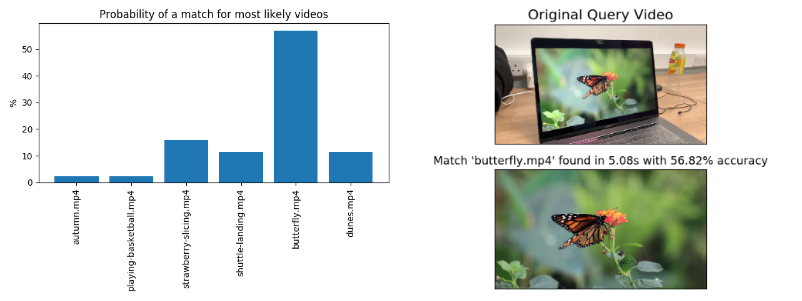
\includegraphics[width=\textwidth]{figures/implementation/online-retrieval-results.png}}
\caption{\label{fig:implementation-online-retrieval-results}Example of the results at the end of the on-line retrieval phase. In the left-hand side is a histogram showing the probability in percentage \% of the most likely videos to match the query. In the right-hand side is a figure presenting the final results, including the first frames of the query video and the match video along with the runtime and the accuracy of the match.}
\end{figure}

Once this figure with the final results is displayed, the program exits, marking the end of the pipeline. The on-line retrieval phase can be repeated any number of times using different query recordings of one of the database videos, without the need to run the off-line colour-based extraction phase again.

%%%%%%%%%%%%%%%%%%%%%%%%%%%%%%%%%%%%%%%%%%%%%%%%%%%%%%%%%%%%%%%%%%%%
%%%%%%%%%%%%%%%%%%%%%%%%%%%%%%%%%%%%%%%%%%%%%%%%%%%%%%%%%%%%%%%%%%%%
%%%%%%%%%%%%%%%%%%%%%%%%%%%%%%%%%%%%%%%%%%%%%%%%%%%%%%%%%%%%%%%%%%%%

\section{Database Pre-Processing}
\label{sec:database-pre-processing}

This section details the steps that go towards processing the database of videos with a shot boundary detection algorithm in order to segment a video. A short twelve-seconds long video made up of four shots is used for this phase of the system, which contains three different types of transitions between each shot, as depicted in Figure \ref{fig:shot_boundary_detection_frames}:

\begin{figure}[h] 
\centerline{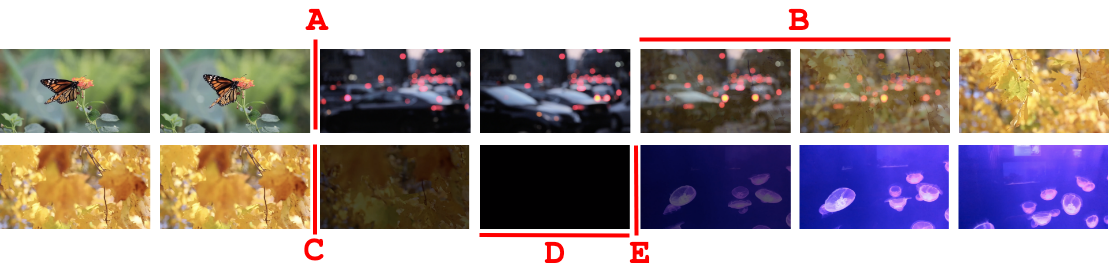
\includegraphics[width=\textwidth]{figures/implementation/shot_boundary_detection_frames.png}}
\caption{\label{fig:shot_boundary_detection_frames}Video frames used for the shot boundary detection algorithm.}
\end{figure}

\begin{itemize}
    \item Quick cut between the butterfly video and the traffic video,
    \item Dissolve cut between the traffic video and the autumn video,
    \item Fade to black cut between the autumn video and the jellyfish video.
\end{itemize}

The shot boundary detection algorithm is implemented using similar techniques described in the two previous phases. RGB histograms are generated for consecutive frames before being compared using distance metrics. The first metric used is the Kullback-Leibler Divergence, followed by the Intersection metric.\\

\subsubsection{Kullback-Leibler Divergence}

The Kullback-Leibler Divergence is normally used to calculate how much information is lost between two distributions, based on Equation \ref{eq:kl-divergence}, but it can nevertheless be used to detect when two consecutive histograms are too distant from one another.
\begin{equation}
\label{eq:kl-divergence}
    d_{KL}(H_1||H_2)=\sum_I H_1(I)\cdot log(\frac{H_1(I)}{H_2(I)})
\end{equation}
Therefore, the RGB histograms of two consecutive frames are generated and compared using the KL Divergence metric for each colour channel in the histogram, which is adapted to the shot boundary detection algorithm in Equation \ref{eq:shot-boundary-detection-kldivergence}. 
\begin{equation}
\label{eq:shot-boundary-detection-kldivergence}
\begin{aligned}
    detection \quad if & \sum_{h}^{(r,g,b)}d_{KL}(H_1||H_2) > t \\
    & \sum_{h}^{(r,g,b)} (\sum_I H_{1,h}(I)\cdot log(\frac{H_{1,h}(I)}{H_{2,h}(I)})) > t
\end{aligned}
\end{equation}
where $t$ is the threshold. If the sum of the three distances is greater the global pre-defined threshold $t=10$, then the two consecutive frames are different enough to be interpreted as a shot change, and the frame index is added to a list of detected shot boundaries. The global threshold of 10 was determined by running the code multiple times to determine a value that detects most of transitions mentioned earlier. This is implemented in the code using the same techniques mentioned in the previous techniques, employing the \textit{cv2.calcHist()} function to generate the histograms for the three colour channels and \textit{cv2.compareHist()} to compare the RGB histograms:

\begin{lstlisting}[numbers=none]
comparison_r = cv2.compareHist(prev_rgb_hist['r'][0], cur_rgb_hist['r'][0], cv2.HISTCMP_KL_DIV)
comparison_g = cv2.compareHist(prev_rgb_hist['g'][0], cur_rgb_hist['g'][0], cv2.HISTCMP_KL_DIV)
comparison_b = cv2.compareHist(prev_rgb_hist['b'][0], cur_rgb_hist['b'][0], cv2.HISTCMP_KL_DIV)
comparison = (comparison_b + comparison_g + comparison_r) / 3
\end{lstlisting}

\begin{figure}[h] 
\centerline{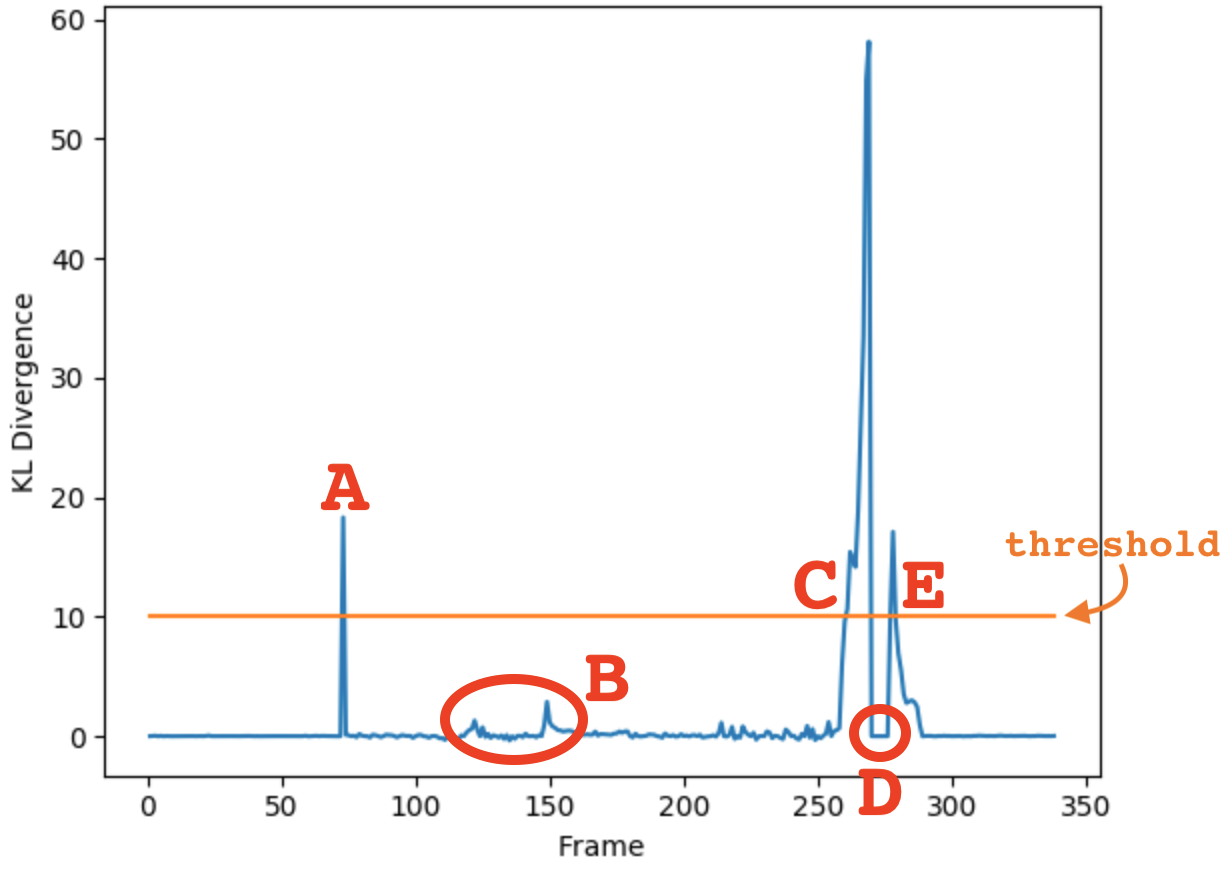
\includegraphics[width=0.70\textwidth]{figures/implementation/shot_boundary_detection_example.png}}
\caption{\label{fig:shot_boundary_detection_example}Example of the shot boundary detection algorithm on the test video from Figure    \ref{fig:shot_boundary_detection_frames} using the Kullback-Leibler Divergence to compare the RGB histograms between consecutive frames.}
\end{figure}

Once the video has been processed, all of the frames with a KL divergence superior to the threshold are marked as shot boundaries. The KL divergence between the consecutive frames from the test video is plotted using Matplotlib, with the results depicted in Figure \ref{fig:shot_boundary_detection_example}.\\

This global threshold approach using KL Divergence to process consecutive frames detects hard cuts \textit{(A)} and fading to black cuts \textit{(C \& E)}, but does not detect a dissolve cut \textit{(B)}. It also detects the black frames in a fading to black transition as a new shot \textit{(D)}.

\subsubsection{Intersection}

The Intersection metric previously explained in Section \ref{sec:implementation-distance-measurements} with Equation \ref{eq:intersection} is also used to calculate the similarities between two consecutive frames in a video, as shown in Equation \ref{eq:shot-boundary-detection-intersection}:
\begin{equation}
\label{eq:shot-boundary-detection-intersection}
\begin{aligned}
    detection \quad if & \sum_{h}^{(r,g,b)}d(H_1,H_2) < t \\
    & \sum_{h}^{(r,g,b)} (\sum_Imin(H_{1,h}(I),H_{2,h}(I))) < t
\end{aligned}
\end{equation}
where $t$ is the threshold. In this case, if the sum of the three distances is smaller than then global threshold $t=7$, then the two consecutive frames are not similar enough to be considered as the same shot, and the frame index is also added to a list of detected shot boundaries. Similarly to the previous technique, the global threshold of 7 was determined by running the code multiple times to find a value than could detect most transitions. \textit{cv2.calcHist()} and \textit{cv2.compareHist()} are once again used to generate and compare the RGB histograms. Once the video has been processed, all the frames with an intersection value smaller than the threshold are marked as shot boundaries, with the results depicted in Figure \ref{fig:shot_boundary_detection_intersection}.\\

\begin{figure}[h] 
\centerline{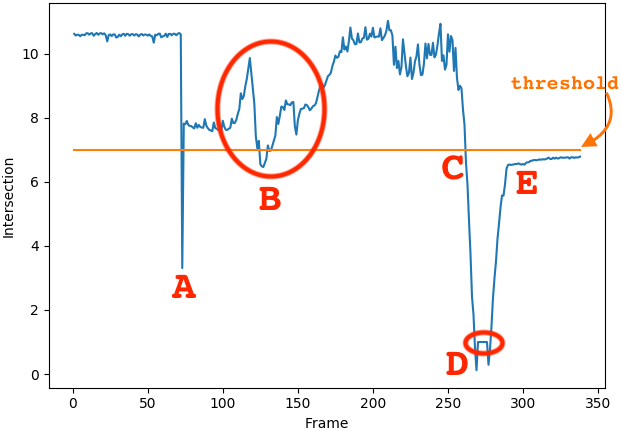
\includegraphics[width=0.70\textwidth]{figures/implementation/shot_boundary_detection_intersection.png}}
\caption{\label{fig:shot_boundary_detection_intersection}Example of the shot boundary detection algorithm on the test video from Figure \ref{fig:shot_boundary_detection_frames} using the Intersection metric to compare the RGB histograms between consecutive frames.}
\end{figure}

This global threshold approach using the Intersection metric to process consecutive frames detects all the transitions in the test video, including the hard cuts \textit{(A)}, the dissolving cut \textit{(B)} and the fading to black cuts \textit{(C \& E)}. However, it also detects the black frames in a fading to black transition as a new shot \textit{(D)}.\\

Despite not being 100\% accurate with the dissolve cut \textit{(B)} not being detected and the black frames being detected as a new shot, the shot boundary detection algorithm is a satisfying method regardless of the metric being used (KL Divergence and Intersection both worked well with the test video). It is especially efficient when using for long videos as the goal is to extract a fraction of the frames rather than generate an exhaustive list of all the shots and scenes in a video. As mentioned earlier in Section \ref{sec:implementation-greyscale-histogram}, this algorithm is not included in the actual pipeline flow as short videos made of single shots and ranging from 7 to 14 seconds are used. However, it is used when testing with longer videos comprised of multiple shots. Supporting code listings covering the code used for this phase can be found in the appendix, including the initial function controlling the execution process of this phase in Appendix \ref{sec:code-database_preprocessing_phase} and the shot boundary detection algorithm in Appendix \ref{sec:code-shot_boundary_detection}.

%%%%%%%%%%%%%%%%%%%%%%%%%%%%%%%%%%%%%%%%%%%%%%%%%%%%%%%%%%%%%%%%%%%%
%%%%%%%%%%%%%%%%%%%%%%%%%%%%%%%%%%%%%%%%%%%%%%%%%%%%%%%%%%%%%%%%%%%%
%%%%%%%%%%%%%%%%%%%%%%%%%%%%%%%%%%%%%%%%%%%%%%%%%%%%%%%%%%%%%%%%%%%%

\section{Complete System Pipeline Flowchart}

Based on the detailed implementation of the system, a flowchart depicting the main aspects of the system can be found in Figure \ref{fig:CBVR-flowchart} towards the end of the chapter.

%%%%%%%%%%%%%%%%%%%%%%%%%%%%%%%%%%%%%%%%%%%%%%%%%%%%%%%%%%%%%%%%%%%%
%%%%%%%%%%%%%%%%%%%%%%%%%%%%%%%%%%%%%%%%%%%%%%%%%%%%%%%%%%%%%%%%%%%%
%%%%%%%%%%%%%%%%%%%%%%%%%%%%%%%%%%%%%%%%%%%%%%%%%%%%%%%%%%%%%%%%%%%%

\section{Development Testing}

This project does not implement a traditional testing suite with unit tests, integration tests and acceptance tests (Priority 3 Requirement F19). Rather than spending time writing an extensive testing suite, which is not very useful considering the nature of the project, the program is repetitively tested before committing changes to GitHub. The test is carried out by using one of the database videos as the query video, which should always match that same video with 100\% accuracy (only true positives, no false positives) and no other potential matches listed (only one video in the histogram). An example of this test is portrayed in Figure \ref{fig:implementation-identity-query}. If an accuracy of 100\% is not achieved, then the system is debugged to rectify mistakes and ensure an accuracy of 100\% when using a database video as the query.

\begin{figure}[h] 
\centerline{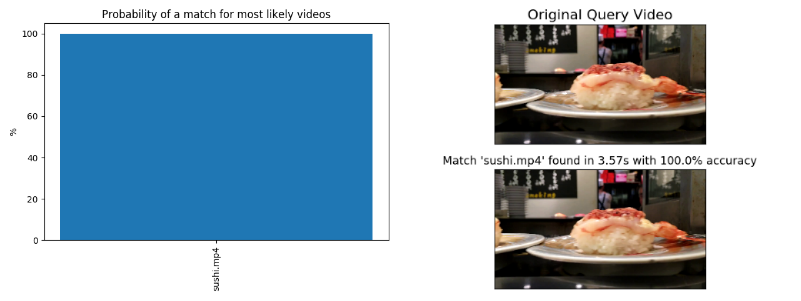
\includegraphics[width=\textwidth]{figures/implementation/identity-query.png}}
\caption{\label{fig:implementation-identity-query}Testing that the system functions as expected before committing changes by using a database video as the input query.}
\end{figure}

%%%%%%%%%%%%%%%%%%%%%%%%%%%%%%%%%%%%%%%%%%%%%%%%%%%%%%%%%%%%%%%%%%%%
%%%%%%%%%%%%%%%%%%%%%%%%%%%%%%%%%%%%%%%%%%%%%%%%%%%%%%%%%%%%%%%%%%%%
%%%%%%%%%%%%%%%%%%%%%%%%%%%%%%%%%%%%%%%%%%%%%%%%%%%%%%%%%%%%%%%%%%%%

\section{Code Structure}

This section covers the project structure of the implemented code, detailing what each directory and file represents. The code, along with the database and testing queries, can be found online on GitHub: \url{https://github.com/Adamouization/Content-Based-Video-Retrieval-Code}.

\begin{itemize}
    \item \textit{``app''} directory: contains all the Python code used to implement the system.
    \begin{itemize}
        \item \textit{``main.py''} file: the starting point of the program. Parses command line arguments to determine whether to run the off-line feature extraction phase, the on-line retrieval phase, or the database pre-processing phase.
        \item \textit{``histogram.py''} file: contains the \textit{HistogramGenerator} class with functions to generate, average, store and compare greyscale, RGB and HSV histograms.
        \item \textit{``video\_operations.py''} file: contains classes for video-related operations. The \textit{ClickAndDrop} class is used for manually selecting the Region of Interest and the \textit{VideoStabiliser} is used to stabilise the query video.
        \item \textit{``helpers.py''} file: contains multiple general-use functions such as retrieving file names, removing file extensions from filenames, displaying the final results in the form of plots or console outputs, parsing command line input and getting video information. The code for the various functions in this module can be found in Appendix \ref{sec:code-helpers-module}.
        \item \textit{``config.py''} file: contains global variables whose values are set by the command line arguments.
        \item \textit{``\_\_init\_\_.py''} file: default file required in any python package (cannot be deleted without causing errors).
    \end{itemize}
    \item \textit{``footage''} directory: where all the database of videos is located. A greyscale, RGB and HSV histogram is generated for each video in this directory. The query's histograms are then compared to each video's histograms from this directory.
    \item \textit{``histogram\_data''} directory: where the averaged greyscale, RGB and HSV histograms are stored as plain text files.
    \item \textit{``recordings''} directory: where all the pre-recorded query videos used to test the system are placed.
    \item \textit{``results''} directory: where general result-related files such as CSV and PNG files are placed.
    \item \textit{``requirements.txt''} file: the different technologies and third-party libraries required to run the code. The file is used by the Pip\footnote{PyPi: \url{https://pypi.org/}} system to install everything in a single installation.
    \item \textit{``README.md''} file: the instructions on how to setup and run the program locally.
\end{itemize}

%%%%%%%%%%%%%%%%%%%%%%%%%%%%%%%%%%%%%%%%%%%%%%%%%%%%%%%%%%%%%%%%%%%%
%%%%%%%%%%%%%%%%%%%%%%%%%%%%%%%%%%%%%%%%%%%%%%%%%%%%%%%%%%%%%%%%%%%%
%%%%%%%%%%%%%%%%%%%%%%%%%%%%%%%%%%%%%%%%%%%%%%%%%%%%%%%%%%%%%%%%%%%%

\section{Summary}

This chapter detailed different steps that were followed to implement the different phases of the system. The off-line colour-based feature extraction phase was first looked at in detail, explaining how the greyscale, RGB and HSV histograms are generated for each database video before being averaged and saved into plain text files. The on-line retrieval phase was next dealt with, revealing the steps followed to pre-process the query video before matching it to one of the database videos through the use of distance metrics and displaying the final result. The database pre-processing phase was inspected last, describing how each database video can be segmented into a fraction of its original size by using a shot boundary detection algorithm. The chapter ended with a detailed diagram betraying the complete system's flowchart, followed by a list of the code's structure and ending on a brief note about testing. With the system completed and working as intended with all the requirements met, the next chapter will test and evaluate the accuracy, quality and scalability of the results for each phase of the system pipeline. 

\begin{figure}[h] 
\centerline{\includegraphics[width=1.20\textwidth]{figures/implementation/full-pipeline-flowchart.png}}
\caption{\label{fig:CBVR-flowchart}Complete flowchart of the system pipeline.}
\end{figure}

% Code can be output inline using \verb@\lstinline|some code|@.  For example,
% this code is inline: \lstinline|public static int example = 0;|  (I have
% used the character \verb@|@ as a delimiter, but any non-reserved character
% not in the code text can be used.)

% Code snippets can be output using the \verb|\begin{lstlisting} ... \end{lstlisting}|
% environment with the code given in the environment.  For
% example, consider listing \ref{Example-Code}, below.

% \begin{lstlisting}[breaklines,breakatwhitespace,caption={Example code},label=Example-Code]
% public static void main() {

%   System.out.println("Hello World");

% }
% \end{lstlisting}

% Code listings are produced using the package ``Listings''.  This has many
% useful options, so have a look at the package documentation for further
% ideas.

% review the outcomes, and critique the outcomes process.
\chapter{Evaluation}
\label{ch:chapter6}
\begin{itemize}
    \item details about the dataset
    \begin{itemize}
        \item test with 50 database videos
        \item query: test with different videos at different angles with +/- hand movement
    \end{itemize}
    
    \item show quantitative values with:
    \begin{itemize}
        \item number of True Positives 
        \item number of False Positives
        \item general accuracy
        \item runtime
    \end{itemize}
    
    \item analyse results of RGB, grey scale and HSV histograms with the 8 different histogram matching methods. Mention which work best?
    
    \item online classification experiment
    \begin{itemize}
        \item Google Survey experiment results 
        \item Compare experiment results with the algorithm results
        \item use a plot to visualise experiment results
        \item link to appendix (Ethics Checklist Appendix \ref{ch:appendix-ethics-checklist}, Experiment Script Appendix \ref{ch:appendix-experiment-survey}, and Raw Results)
    \end{itemize}
\end{itemize}

mention ground truth (https://en.wikipedia.org/wiki/Ground\_truth) (https://www.techopedia.com/definition/32514/ground-truth)

\chapter{Discussion}
\label{ch:chapter7}
\begin{itemize}
    \item state what could be improved with time
    \begin{itemize}
        \item region-based histograms, separate frame in 5 regions and generate a histogram for each region rather than having a global histogram to describe the frame (https://www.pyimagesearch.com/2014/12/01/complete-guide-building-image-search-engine-python-opencv/)
        \item improve ROI selection to take 4 points rather than 2 (will increase accuracy for query videos that are at an angle, not filming the screen from a straight point of view)
        \item automatic ROI detection (detect screen edges with edge and corner detector algorithms)
        \item more features to complement the colour-based features (e.g. motion and shape features) and improve the accuracy
        \item make use of sound to further improve accuracy
        \item GUI e.g. Tkinter application or simple HTML webpage
    \end{itemize} 
    \item mention that with improvements, could have worked with small database of movies rather than short videos
    \item limitations of working with large database of movies: 
    \begin{itemize}
        \item too much data to process, could perhaps be pre-processed in advance
        \item copyright issues of having all these movies
    \end{itemize}
\end{itemize}

\chapter{Conclusions}
\label{ch:chapter8}
This is the chapter in which you review the major achievements in the
light of your original objectives, critique the process, critique your
own learning and identify possible future work.

\bibliography{Bibliography}

\let\cleardoublepage\clearpage % don't automatically start appendix chapters on odd pages
\appendix

\chapter{Comparison Between Potential Programming Languages}
\label{ch:appendix-comparison-programming-languages}
\begin{longtable}[c]{l|l|l|l|l|}
\cline{2-5}
 & \multicolumn{1}{c|}{\textbf{Python}} & \multicolumn{1}{c|}{\textbf{C++}} & \multicolumn{1}{c|}{\textbf{Java}} & \multicolumn{1}{c|}{\textbf{MATLAB}} \\ \hline
\endfirsthead
%
\multicolumn{5}{c}%
{{\bfseries Table \thetable\ continued from previous page}} \\
\endhead
%
\multicolumn{1}{|l|}{Familiarity} & \begin{tabular}[c]{@{}l@{}}Very familiar:\\ used in industry \\ and personal \\ projects\end{tabular} & Unfamiliar & \begin{tabular}[c]{@{}l@{}}Familiar in the \\ past: used in \\ industry and \\ coursework\end{tabular} & \begin{tabular}[c]{@{}l@{}}Somewhat \\ familiar\end{tabular} \\ \hline
\multicolumn{1}{|l|}{\begin{tabular}[c]{@{}l@{}}Support for \\ video\\ manipulation \\ and \\ computer \\ vision \\ functions\end{tabular}} & \begin{tabular}[c]{@{}l@{}}OpenCV \\ library \\ support\end{tabular} & \begin{tabular}[c]{@{}l@{}}OpenCV \\ library \\ support\end{tabular} & \begin{tabular}[c]{@{}l@{}}OpenCV \\ library \\ support\end{tabular} & \begin{tabular}[c]{@{}l@{}}Native video \\ manipulation \\ and computer \\ vision functions\end{tabular} \\ \hline
\multicolumn{1}{|l|}{Speed*} & \begin{tabular}[c]{@{}l@{}}Slow** \\ (interpreted)\end{tabular} & \begin{tabular}[c]{@{}l@{}}Very fast \\ (compiled)\end{tabular} & \begin{tabular}[c]{@{}l@{}}Fast \\ (compiled)\end{tabular} & \begin{tabular}[c]{@{}l@{}}Slow \\ (interpreted)\end{tabular} \\ \hline
\multicolumn{1}{|l|}{\begin{tabular}[c]{@{}l@{}}Code \\ Readability\end{tabular}} & \begin{tabular}[c]{@{}l@{}}Simple syntax \\ to follow, \\ easy to read***\end{tabular} & \begin{tabular}[c]{@{}l@{}}Complex and \\ wordy syntax\end{tabular} & \begin{tabular}[c]{@{}l@{}}Complex and \\ wordy syntax\end{tabular} & \begin{tabular}[c]{@{}l@{}}Complex \\ syntax\end{tabular} \\ \hline
\caption{Table comparing the main pros and cons for using different programming languages to build the system.}
\end{longtable}

* Based on \textit{Benchmarks Game}\footnote{\url{https://benchmarksgame-team.pages.debian.net/benchmarksgame/}} and \textit{``A Comparison of Programming Languages'', J. Kinlay}\footnote{\url{http://jonathankinlay.com/2018/10/comparison-programming-languages/}}.\\

** Python code using OpenCV functions executes as fast as the original OpenCV library C++ code since it is the actual OpenCV C++ code that is running in the background, thus maintaining high-speed despite using Python\footnote{OpenCV Python Tutorials, \url{https://opencv-python-tutroals.readthedocs.io/en/latest/py\_tutorials/py\_setup/py\_intro/py\_intro.html\#intro}}.\\

*** Following the PEP8 coding style guide will ensure that code readable by professionals will be written, meeting the goal set by requirement F21 in Chapter \ref{ch:chapter3}.

\chapter{Comparison Between Text and Binary Files}
\label{ch:appendix-comparison-text-vs-binary}
% Please add the following required packages to your document preamble:
\begin{table}[h]
\centering
\begin{tabular}{@{}ll@{}}
\toprule
\multicolumn{1}{c}{\textbf{Text files}} & \multicolumn{1}{c}{\textbf{Binary files}} \\ \midrule
\multicolumn{1}{|l|}{Are human readable: text files are easier to debug since people can see what was written to the file.} & \multicolumn{1}{l|}{Are not human readable: binary files are a lot more difficult to debug because people cannot easily see what was written to the file.} \\ \midrule
\multicolumn{1}{|l|}{When dealing with large data, compression may be a factor. For example, 10-digits number will take at least 10 bytes as text.} & \multicolumn{1}{l|}{\begin{tabular}[c]{@{}l@{}}Will store the same data in less space. For example: 10-digits number will take as\\ little as four or two as binary.\end{tabular}} \\ \midrule
\multicolumn{1}{|l|}{More restrictive than binary files since they can only contain textual data.} & \multicolumn{1}{l|}{Binary file formats are less restrictive as they may include multiple types of data in the same file such as image, video, and audio data.} \\ \midrule
\multicolumn{1}{|l|}{Less likely to become corrupted. A small error in a text file may simply show up once the file has been opened.} & \multicolumn{1}{l|}{More likely to become corrupted. A small error in a binary file may make it unreadable.} \\ \midrule
Many programs are capable of reading and editing text files. & Less programs are capable of reading and editing text files. \\ \bottomrule
\end{tabular}
\end{table}

\chapter{Code Listings}
\label{ch:appendix-code-listings}
This appendix includes the main code sections of the system in a lightweight form, with omitted comments and condensed formats. The code is organised by module.

%%%%%%%%%%%%%%%%%%%%%%%%%%%%%%%%%%%%%%%%%%%%%%%%%%%%%%%%%%%%%%%%%%%%%%%%%%%%%%%%%%
%%%%%%%%%%%%%%%%%%%%%%%%%%%%%%%%%%%%%% MAIN %%%%%%%%%%%%%%%%%%%%%%%%%%%%%%%%%%%%%%
%%%%%%%%%%%%%%%%%%%%%%%%%%%%%%%%%%%%%%%%%%%%%%%%%%%%%%%%%%%%%%%%%%%%%%%%%%%%%%%%%%

\section{Main Module}

The \textit{main.py} module contains the program entry point that parses the command line argument in order to decide which phase to execute. Contains the three functions to begin each phase, include the off-line colour-based feature extraction, the on-line retrieval and database pre-processing phases.

\subsection{Argument Parsing}
\label{sec:code-listings-argument-parsing}

The program entry point. Parses command line input to decide which phase of the system to run.

\lstinputlisting{code-listings/main/argument_parsing.py}

%%%%%%%%%%%%%%%%%%%%%%%%%%%%%%%%%%%%%%%%%

\subsection{Initial Off-line Colour-based Feature Extraction Phase Function}
\label{sec:code-off_line_colour_based_feature_extraction_phase}

Generates and stores averaged greyscale, RGB and HSV histograms for all the videos in the directory-based database.

\lstinputlisting{code-listings/main/off_line_colour_based_feature_extraction_phase.py}

%%%%%%%%%%%%%%%%%%%%%%%%%%%%%%%%%%%%%%%%%

\subsection{Initial On-line Retrieval Phase Function}
\label{sec:code-on_line_retrieval_phase}

Prompts the user to stabilise and crop the query video before generating the same averaged greyscale, RGB and HSV histograms to compare with the database videos' previously stored histograms using distance metrics.

\lstinputlisting{code-listings/main/on_line_retrieval_phase.py}

%%%%%%%%%%%%%%%%%%%%%%%%%%%%%%%%%%%%%%%%%

\subsection{Initial Database Pre-Processing Phase}
\label{sec:code-database_preprocessing_phase}

Applies a shot boundary detection algorithm to a video for segmentation.

\lstinputlisting{code-listings/main/database_preprocessing_phase.py}

%%%%%%%%%%%%%%%%%%%%%%%%%%%%%%%%%%%%%%%%%%%%%%%%%%%%%%%%%%%%%%%%%%%%%%%%%%%%%%%%%%
%%%%%%%%%%%%%%%%%%%%%%%%%%%%%%%%%%% HISTOGRAMS %%%%%%%%%%%%%%%%%%%%%%%%%%%%%%%%%%%
%%%%%%%%%%%%%%%%%%%%%%%%%%%%%%%%%%%%%%%%%%%%%%%%%%%%%%%%%%%%%%%%%%%%%%%%%%%%%%%%%%

\clearpage
\section{Histograms Module}

The \textit{histogram.py} module contains the HistogramGenerator class with functions to generate, average, store and compare greyscale, RGB and HSV histograms.

%%%%%%%%%%%%%%%%%%%%%%%%%%%%%%%%%%%%%%%%%

\subsection{High Level Module Overview}
\label{sec:code-high-level-module-overview}

A high-level overview of the module's classes and functions.

\lstinputlisting{code-listings/histogram/histogram_module_high_level.py}

%%%%%%%%%%%%%%%%%%%%%%%%%%%%%%%%%%%%%%%%%

\subsection{Single Greyscale Histogram Generation}
\label{sec:code-single_grey_histogram_generation}

Generates multiple greyscale histograms (one every second) for a video.

\lstinputlisting{code-listings/histogram/single_grey_histogram_generation.py}

%%%%%%%%%%%%%%%%%%%%%%%%%%%%%%%%%%%%%%%%%

\subsection{Single RGB Histogram Generation}
\label{sec:code-single_rgb_histogram_generation}

Generates multiple RGB histograms (one every second) for a video.

\lstinputlisting{code-listings/histogram/single_rgb_histogram_generation.py}

%%%%%%%%%%%%%%%%%%%%%%%%%%%%%%%%%%%%%%%%%

\subsection{Single HSV Histogram Generation}
\label{sec:code-average_and}

Generates multiple HSV histograms (one every second) for a video.

\lstinputlisting{code-listings/histogram/single_hsv_histogram_generation.py}

%%%%%%%%%%%%%%%%%%%%%%%%%%%%%%%%%%%%%%%%%

\subsection{Average \& Store Greyscale Histogram}
\label{sec:code-generate_and_store_average_grey_histogram}

Generates a single greyscale histogram by averaging all histograms of a video before normalising it and saving the results to a plain text file.

\lstinputlisting{code-listings/histogram/generate_and_store_average_grey_histogram.py}

%%%%%%%%%%%%%%%%%%%%%%%%%%%%%%%%%%%%%%%%%

\subsection{Average \& Store RGB Histogram}
\label{sec:code-generate_and_store_average_rgb_histogram}

Generates a single RGB histogram by averaging all histograms of a video before normalising it and saving the results to a plain text file.

\lstinputlisting{code-listings/histogram/generate_and_store_average_rgb_histogram.py}

%%%%%%%%%%%%%%%%%%%%%%%%%%%%%%%%%%%%%%%%%

\subsection{Average \& Store HSV Histogram}
\label{sec:code-generate_and_store_average_hsv_histogram}

Generates a single HSV histogram by averaging all histograms of a video before normalising it and saving the results to a plain text file.

\lstinputlisting{code-listings/histogram/generate_and_store_average_hsv_histogram.py}

%%%%%%%%%%%%%%%%%%%%%%%%%%%%%%%%%%%%%%%%%

\subsection{Matching 2D Histograms}
\label{sec:code-match_2D_histograms}

describe

\lstinputlisting{code-listings/histogram/match_2D_histograms.py}

%%%%%%%%%%%%%%%%%%%%%%%%%%%%%%%%%%%%%%%%%

\subsection{Matching 3D Histograms}
\label{sec:code-match_3D_histograms}

describe

\lstinputlisting{code-listings/histogram/match_3D_histograms.py}

%%%%%%%%%%%%%%%%%%%%%%%%%%%%%%%%%%%%%%%%%

\subsection{Shot Boundary Algorithm}
\label{sec:code-shot_boundary_detection}

Compares consecutive frames' RGB histograms using the Intersection metric with a global threshold approach. If the metric is smaller than the specified threshold, then a shot boundary has been detected.

\lstinputlisting{code-listings/histogram/shot_boundary_detection.py}

%%%%%%%%%%%%%%%%%%%%%%%%%%%%%%%%%%%%%%%%%

\subsection{Frames Pre-Selection Function}
\label{sec:code-get_frames_to_process}

Returns the IDs of the frames to calculate a histogram for (1 frame per second).

\lstinputlisting{code-listings/histogram/get_frames_to_process.py}

%%%%%%%%%%%%%%%%%%%%%%%%%%%%%%%%%%%%%%%%%%%%%%%%%%%%%%%%%%%%%%%%%%%%%%%%%%%%%%%%%%
%%%%%%%%%%%%%%%%%%%%%%%%%%%%%%%% VIDEO OPERATIONS %%%%%%%%%%%%%%%%%%%%%%%%%%%%%%%%
%%%%%%%%%%%%%%%%%%%%%%%%%%%%%%%%%%%%%%%%%%%%%%%%%%%%%%%%%%%%%%%%%%%%%%%%%%%%%%%%%%

\clearpage
\section{Video Operations Module}

The \textit{video\_operations.py} module contains the code used to perform operations on the query video. It takes care of the pre-processing steps, including video stabilisation and manual ROI selection. 

%%%%%%%%%%%%%%%%%%%%%%%%%%%%%%%%%%%%%%%%%

\subsection{VideoStabiliser Class}
\label{sec:code-VideoStabiliser}

Class used to stabilise the recorded video for more optimal matching.

\lstinputlisting{code-listings/video_operations/VideoStabiliser.py}

%%%%%%%%%%%%%%%%%%%%%%%%%%%%%%%%%%%%%%%%%

\subsection{ClickAndDrop Class for Manual ROI Selection}
\label{sec:code-ClickAndDrop}

Class for selecting a region of interest on a frame by click and dropping the mouse over the desired area, and cropping that frame to include the pixels inside the ROI only.

\lstinputlisting{code-listings/video_operations/ClickAndDrop.py}

%%%%%%%%%%%%%%%%%%%%%%%%%%%%%%%%%%%%%%%%%%%%%%%%%%%%%%%%%%%%%%%%%%%%%%%%%%%%%%%%%%
%%%%%%%%%%%%%%%%%%%%%%%%%%%%%%%%%%%%% HELPERS %%%%%%%%%%%%%%%%%%%%%%%%%%%%%%%%%%%%
%%%%%%%%%%%%%%%%%%%%%%%%%%%%%%%%%%%%%%%%%%%%%%%%%%%%%%%%%%%%%%%%%%%%%%%%%%%%%%%%%%

\clearpage
\section{Helpers Module}

describe module

%%%%%%%%%%%%%%%%%%%%%%%%%%%%%%%%%%%%%%%%%

% \section{Generate Single Histogram}
% \label{sec:code-generate-single-histogram}

% \lstinputlisting[caption=Function generating histograms for the pre-selected frames and adding them to lists before averaging them to create a video's compact signature.]{code-listings/generate_single_histogram.py}

%%%%%%%%%%%%%%%%%%%%%%%%%%%%%%%%%%%%%%%%%


\chapter{13 Point Ethics Check List}
\label{ch:appendix-ethics-checklist}
This document describes the 13 issues that need to be considered carefully before students or staff  involve other people (``participants'') for the collection of information as part of their project or research.

\begin{enumerate}
    \item \textbf{Have you prepared a briefing script for volunteers}?\\
    All participants will be introduced with a briefing script explaining what the project consists of, what their role in the experiment is, and how their data will be used.
    \item \textbf{Will the participants be using any non-standard hardware?}\\
    No. Participants can conduct the experiment from their personal computers or mobile devices.
    \item \textbf{Is there any intentional deception of the participants?}\\
    No deception will occur during this experiment; all the details of the experiment will be provided in the debriefing script.
    \item \textbf{How will participants voluntarily give consent?}\\
    The participants will give consent when they submit their Google Form survey, which is specified in the briefing script.
    \item \textbf{Will the participants be exposed to any risks greater than those encountered in their normal work life?}\\
    Participants will take part in the experiment from their environment of choice as they will receive a link to the online survey in their inbox, which they can use to access the survey online from their personal computers and mobile devices.
    \item \textbf{Are you offering any incentive to the participants?}\\
    No incentive will be offered to participants.
    \item \textbf{Are any of your participants under the age of 16?}\\
    All participants are above the age of 18.
    \item \textbf{Do any of your participants have an impairment that will limit their understanding or communication?}\\
    None of the participants have any known impairment which may affect the experiment's results.
    \item \textbf{Are you in a position of authority or influence over any of your     participants?}\\
    The participants will complete the survey in their own free time using their hardware with no presence of authority present during the experiment.
    \item \textbf{Will the participants be informed that they could withdraw at any time?}\\
    All the participants will be informed that they can withdraw from the experiment at any time in the briefing script.
    \item \textbf{Will the participants be informed of your contact details?}
    My contacts details and my supervisor's details will be shared with all participants.
    \item \textbf{Will participants be de-briefed?}\\
    All participants will be debriefed through the introductory briefing script.
    \item \textbf{Will the data collected from the participants be stored in an anonymous form?}\\
    The data collected from the online survey will be downloaded and stored locally in a CSV file anonymously and will be used anonymously in the final report, as informed in the briefing script.
\end{enumerate}

\chapter{Experiment Survey}
\label{ch:appendix-experiment-survey}
This chapter presents the survey used for the online experiment. The database videos and the query video are included in the survey using YouTube. The online survey is powered by Google Forms, and is available online: \url{https://forms.gle/HyQAGyks2Tnj7wgc9}

\section{Title}

Content-Based Video Retrieval Experiment

\section{What is the project about?}

This dissertation project aims to create a system similar to Shazam for movies.\\

For background information, Shazam is a mobile application that allows users to match a recording to a piece of music.\\

The goal of this project is to explore how such a system could be developed to work with movies, where a user would record a screen with his phone, which will pattern match the movie to a database of movies and accurately return the movie title.

\section{Your role in this experiment}

In this experiment, you play the role of the algorithm that matches a user recording to one of the videos in the database.\\

You will be shown 6 videos from the database, followed by 1 user-recorded video.
Your goal is to mentally compare the recorded video to each video in the database to be able to rank each database video from most likely to match the recorded video to least likely.\\

When making your decision, take into account aspects of the video such as colour distribution, luminosity, textures, shapes, objects and motion, as a video matching algorithm would in real life.\\

Note: The data retrieved from this experiment will be compared to the results the of the project's matching algorithm. It will remain anonymous in locally-stored hard copies and in the final report. By submitting this form, you give consent for your data to be evaluated and used in the report. You may withdraw from the experiment at any time.

\section{Watch}

\paragraph{Database Videos}

Watch the 6 database videos that will train your ``knowledge''.

\begin{figure}[h] 
\centerline{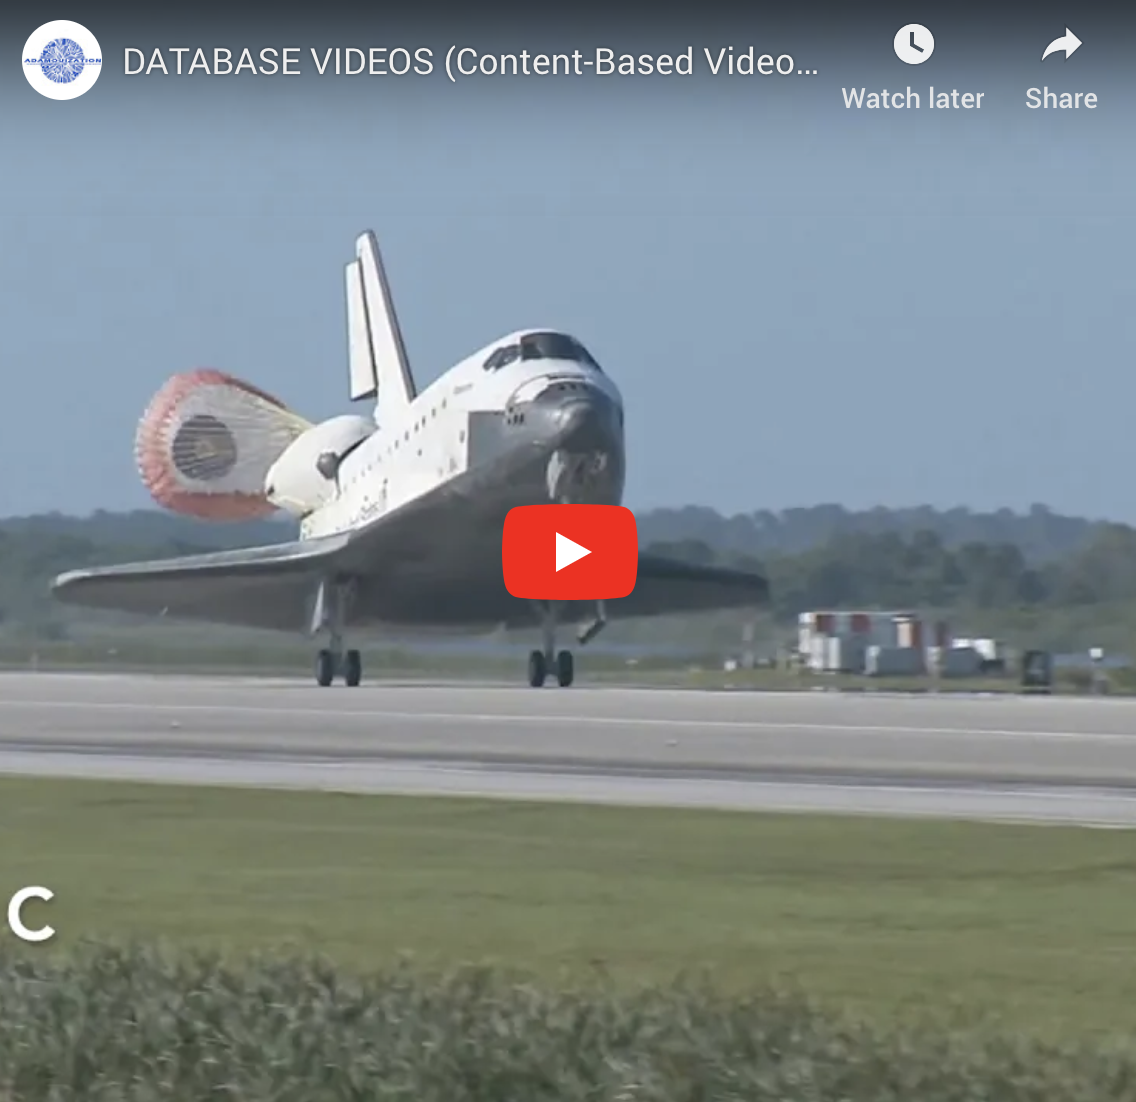
\includegraphics[width=0.50\textwidth]{figures/appendix/survey_db_videos.png}}
\caption{\label{fig:appendix-survey_db_videos}The YouTube video showing the 6 database videos used for the experiment, available online: \url{https://www.youtube.com/watch?v=BvukbK-sX9A}.}
\end{figure}

\paragraph{Query Video}

Now watch the recorded query video. Your goal is now to compare this video to the 6 previous videos you watched and to rank them based on their visual similarities.

\begin{figure}[h] 
\centerline{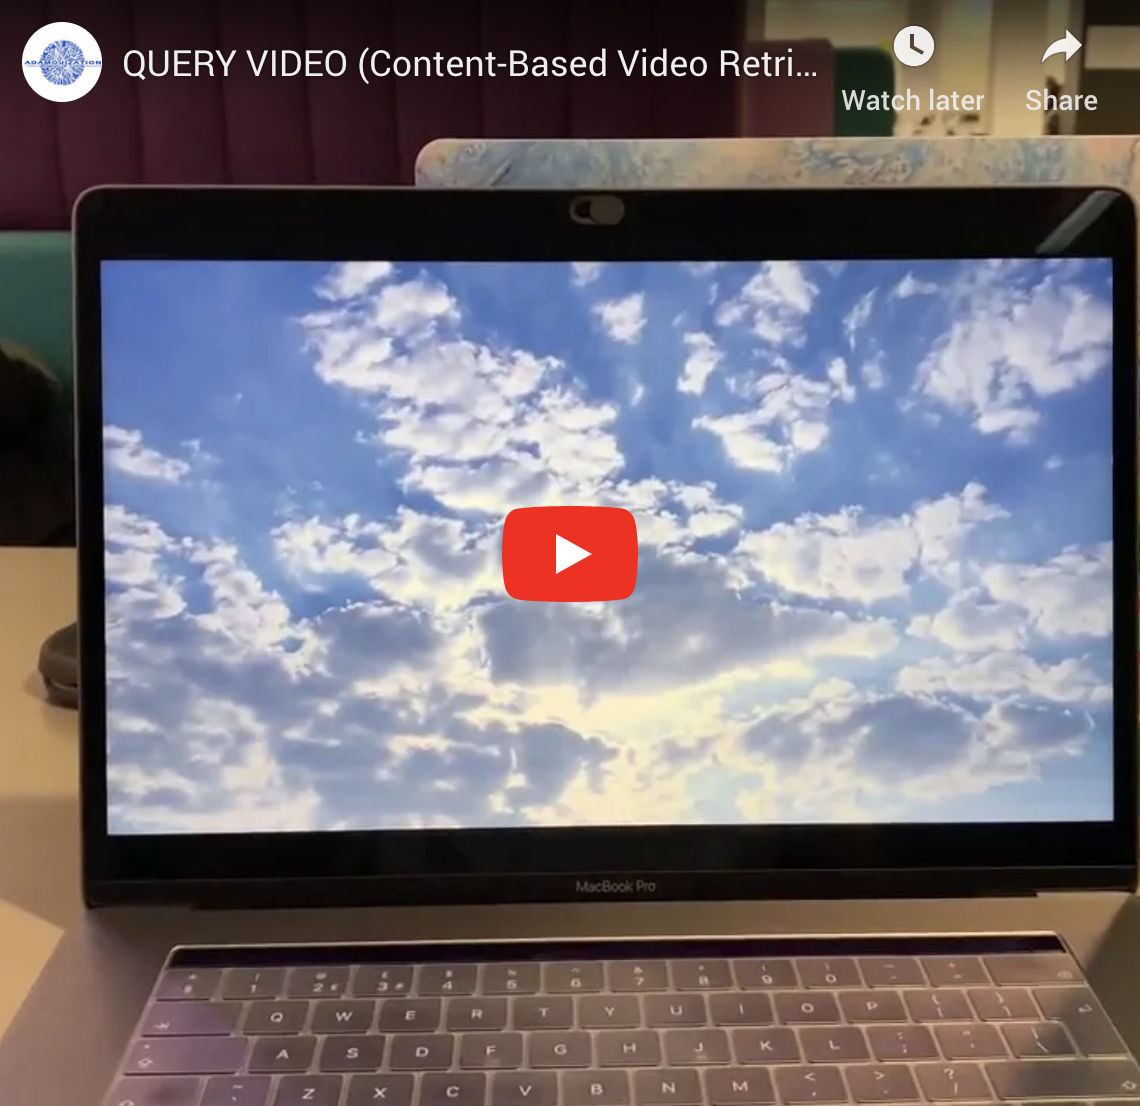
\includegraphics[width=0.5\textwidth]{figures/appendix/survey_query_video.png}}
\caption{\label{fig:appendix-survey_query_video}The YouTube video showing the query video used for the experiment, available online: \url{https://www.youtube.com/watch?v=4JPo0-aSzNE}.}
\end{figure}

\section{Rank}

\textbf{Which database video does the recorded query match the most?}\\

\begin{figure}[h] 
\centerline{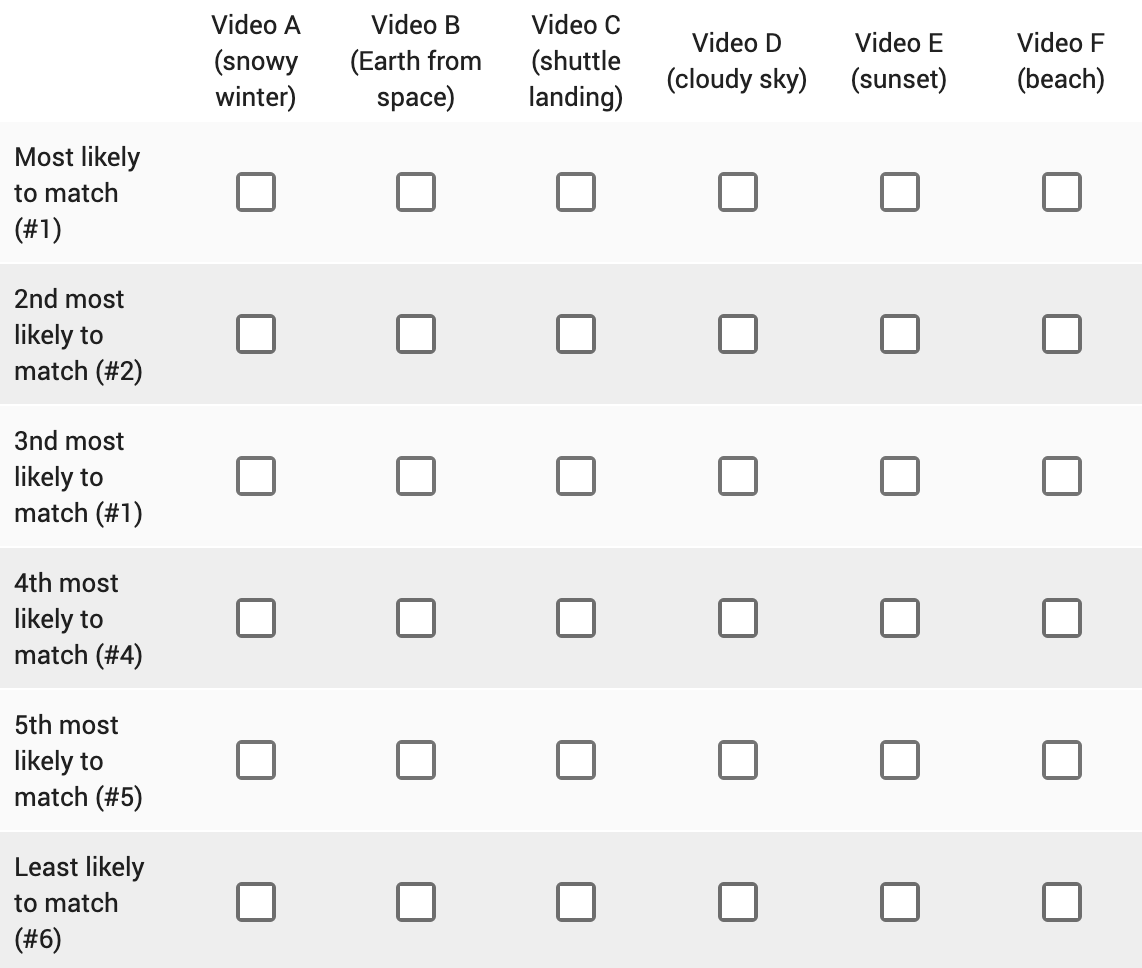
\includegraphics[width=0.55\textwidth]{figures/appendix/survey_video_ranking.png}}
\caption{\label{fig:appendix_survey_video_ranking}Screenshot of the checkbox grid used to rank the database videos from most likely to match the query video to least likely.}
\end{figure}

\textbf{Which video aspects did you consider the most when ranking them?}\\

Placeholder for long answer from participant.\\

\textbf{What do you think is the most important aspect of a video that a matching algorithm should analyse when pattern matching videos?}\\

Placeholder for short answer from participant.

\section{Confirmation Message}

(The message that is displayed to users once they have finished the experiment and submitted the Google Form).\\

\begin{quote}
    Your response has been recorded.\\

    Thank you taking part in this experiment!\\
    
    Here are my algorithm's results for comparison: 
    \begin{enumerate}
        \item cloudy-sky (video D)
        \item winter (video A)
        \item earth (video B)
        \item shuttle-landing (video C)
        \item beach (video F)
        \item sunset (video E)
    \end{enumerate}
    
    Contact details:
    \begin{itemize}
        \item Adam Jaamour: \textit{aj645@bath.ac.uk}
        \item Dr. Yong-Liang Yang (project supervisor): \textit{Y.Yang2@bath.ac.uk}
    \end{itemize}
\end{quote}

\chapter{Raw Experiment Results}
\label{ch:appendix-survey-results}
\section{Which database video does the recorded query match the most?}

\begin{figure}[h] 
\centerline{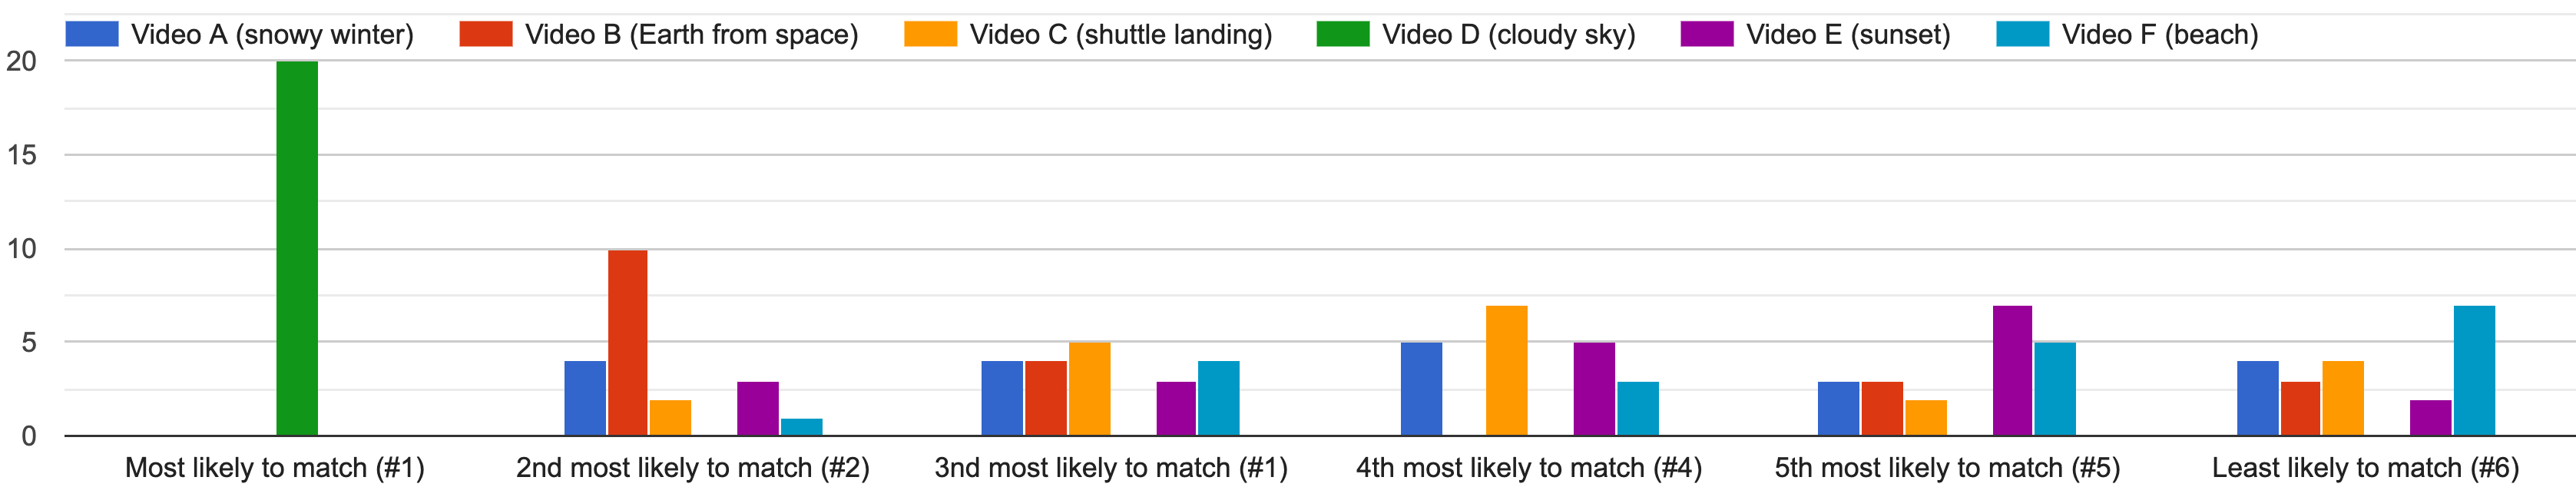
\includegraphics[width=\textwidth]{figures/appendix/survey_results.png}}
\caption{\label{fig:appendix_survey_results}Survey results of the ``Which database video does the recorded query match the most?'' ranking question.}
\end{figure}

\section{Which video aspects did you consider the most when ranking them?}

\begin{itemize}
	\item Participant 1: Blue colour
    \item Participant 2: the sky is cold
    \item Participant 3: The colours and movements
    \item Participant 4: The colour of the sky and the movements
    \item Participant 5: Colors and luminosity
    \item Participant 6: The actual scenario i.e. the fact that a plane was landing or the fact that someone was walking a dog
    \item Participant 7: Light, sky and clouds
    \item Participant 8: clouds
    \item Participant 9: colour, landscape, sounds
    \item Participant 10: movement, patterns, image, colour
    \item Participant 11: luminosity of colours and similarity of object represented
    \item Participant 12: Images, absence of sound, speed of movement
    \item Participant 13: Colors
    \item Participant 14: Colour, movement, size of objects, shape of objects
    \item Participant 15: Image, colour, light
    \item Participant 16: The colors (including luminosity) then the movements
    \item Participant 17: colour blue with blurry whites. sky clearly visible in daytime
    \item Participant 18: The movement and colour of the image
    \item Participant 19: Colours
    \item Participant 20: Colours of the video
\end{itemize}

\section{What do you think is the most important aspect of a video that a matching algorithm should analyse when pattern matching videos?}

\begin{itemize}
	\item Participant 1: Similar colours, shades of colours
    \item Participant 2: colours (warm vs cold) 
    \item Participant 3: Colours 
    \item Participant 4: Colours and the pace of movement and change
    \item Participant 5: Colors
    \item Participant 6: colour
    \item Participant 7: The environment surrounding the action
    \item Participant 8: overall colour and location of major colour blobs
    \item Participant 9: filter / colors, sounds (as many movies can relate similar situation e.g. Second World War, they can be differentiated by determining how old is the movie and where it takes place). Sounds are very different from one movie to another, even in the same topic, so I believe that it is another core aspect to be analyzed.
    \item Participant 10: movement 
    \item Participant 11: shapes and luminosity 
    \item Participant 12: Image + speed of movement 
    \item Participant 13: Colors / Shapes / moving objects
    \item Participant 14: Colour scheme
    \item Participant 15: Sound, quality of image
    \item Participant 16: The motion and the colors
    \item Participant 17: objects appearing in video
    \item Participant 18: The succession of images
    \item Participant 19: movements
    \item Participant 20: Shape and colour of objects within the video
\end{itemize}



% \chapter{Design Diagrams}

% \chapter{User Documentation}

% \chapter{Raw results output}

\end{document}